\documentclass[12pt,spanish,fleqn,openany,letterpaper,pagesize]{scrbook}

\usepackage[utf8]{inputenc}
\usepackage[spanish]{babel}%escribir con acentos sin necesidad de comandos \'{} .
\usepackage{fancyhdr}
\usepackage{epsfig}
\usepackage{epic}
\usepackage{eepic}
\usepackage{amsmath}
\usepackage{threeparttable}
\usepackage{amscd}
\usepackage{here}
\usepackage{graphicx}
\usepackage{lscape}
\usepackage{tabularx}
\usepackage{subfigure}
\usepackage{longtable}
\usepackage{xcolor}

\usepackage{rotating} %Para rotar texto, objetos y tablas seite. No se ve en DVI solo en PS. Seite 328 Hundebuch
                        %se usa junto con \rotate, \sidewidestable ....
\usepackage{mathtools}

\renewcommand{\theequation}{\thechapter-\arabic{equation}}
\renewcommand{\thefigure}{\textbf{\thechapter-\arabic{figure}}}
\renewcommand{\thetable}{\textbf{\thechapter-\arabic{table}}}


\pagestyle{fancyplain}%\addtolength{\headwidth}{\marginparwidth}
\textheight22.5cm \topmargin0cm \textwidth16.5cm
\oddsidemargin0.5cm \evensidemargin-0.5cm%
\renewcommand{\chaptermark}[1]{\markboth{\thechapter\; #1}{}}
\renewcommand{\sectionmark}[1]{\markright{\thesection\; #1}}
\lhead[\fancyplain{}{\thepage}]{\fancyplain{}{\rightmark}}
\rhead[\fancyplain{}{\leftmark}]{\fancyplain{}{\thepage}}
\fancyfoot{}
\thispagestyle{fancy}%


\addtolength{\headwidth}{0cm}
\unitlength1mm %Define la unidad LE para Figuras
\mathindent0cm %Define la distancia de las formulas al texto,  fleqn las descentra
\marginparwidth0cm
\parindent0cm %Define la distancia de la primera linea de un parrafo a la margen

%Para tablas,  redefine el backschlash en tablas donde se define la posici\'{o}n del texto en las
%casillas (con \centering \raggedright o \raggedleft)
\newcommand{\PreserveBackslash}[1]{\let\temp=\\#1\let\\=\temp}
\let\PBS=\PreserveBackslash

%Espacio entre lineas
\renewcommand{\baselinestretch}{1.1}

%Neuer Befehl f\"{u}r die Tabelle Eigenschaften der Aktivkohlen
\newcommand{\arr}[1]{\raisebox{1.5ex}[0cm][0cm]{#1}}

%Neue Kommandos
\usepackage{Befehle}
%Inicio del documento. Tener en cuenta que hay archivos auxiliares

\begin{document}
\pagenumbering{roman}
%\newpage
%\setcounter{page}{1}
\DeclareFontShape{OT1}{cmss}{bx}{sc}{<-> cmbcsc10}{}

\begin{center}
\begin{figure}
\centering%

\epsfig{file=HojaTitulo/EscudoUN,scale=1}%
\end{figure}
\thispagestyle{empty} \vspace*{2.0cm} \textbf{\huge
Multiagent Control of Autonomous Vehicles in Presence of Non-Cooperative Agents Using
Game Theory}\\[5.0cm]
\Large\textbf{Nestor Ivan Ospina Gaitan}\\[5.0cm]
\small Universidad Nacional de Colombia\\
Engineering Faculty, Electronic and Electric Engineering Department.\\
Bogotá, Colombia\\
A\~{n}o 2022\\
\end{center}

%\newpage{\pagestyle{empty}\cleardoublepage}

\newpage
\begin{center}
\thispagestyle{empty} \vspace*{0cm} \textbf{\huge
Multiagent Control of Autonomous Vehicles in Presence of Non-Cooperative Agents Using
Game Theory}\\[3.0cm]
\Large\textbf{Nestor Ivan Ospina Gaitan}\\[2.0cm]
\small Thesis presented as partial requirement for apply to the tittle of:\\
\textbf{Master in Industrial Automation}\\[2cm]
Advisor(a):\\
Ph.D.Eduardo Alirio Mojica Nava\\
Co-Advisor:\\
Ph.D. Duvan Andres Tellez\\[2.0cm]
Research Line:\\
Control and Robotics\\
Research Group:\\
PAAS - Processing, Acquisition and Analysis of Signals\\[1.5cm]
Universidad Nacional de Colombia\\
Engineering Faculty, Electronic and Electric Engineering Department\\
Bogotá, Colombia\\
A\~{n}o 2022\\
\end{center}

%\newpage{\pagestyle{empty}\cleardoublepage}

%\newpage
\thispagestyle{empty} \textbf{}\normalsize
\vspace{1.5cm}%
% \textbf{Dedication}\vspace{4.5cm}

\begin{flushright}
\begin{minipage}{8cm}
    \noindent
        \small
    %    Su uso es opcional y cada autor podr\'{a} determinar la distribuci\'{o}n del texto en la p\'{a}gina, se sugiere esta presentaci\'{o}n. En ella el autor dedica su trabajo en forma especial a personas y/o entidades.\\[1.0cm]\\
    %    Por ejemplo:\\[1.0cm]
        % A mis padres\vspace{1.5cm}
        %o\\[1.0cm]
      %  La preocupaci\'{o}n por el hombre y su destino siempre debe ser el
      %  inter\'{e}s primordial de todo esfuerzo t\'{e}cnico. Nunca olvides esto
      %  entre tus diagramas y ecuaciones.\vspace{1.5cm}
     %   Albert Einstein\\
\end{minipage}
\end{flushright}

%\newpage{\pagestyle{empty}\cleardoublepage}

\newpage
\thispagestyle{empty} \textbf{}\normalsize
\vspace{1.5cm}%
\textbf{\LARGE Acknowledgements}
\addcontentsline{toc}{chapter}{\numberline{}Acknowledgements}
\vspace{2cm}
\\
I want to thank Professor Eduardo Alirio Mojica and Co-advisor D\'uvan Andr\'ez T\'ellez for their unconditional help all these years. To Professor Juan Calderon and Ing Gustavo Cardona for their knowledge, motivation, and support in achieving this goal. Finally, to my mother and brother for always being emotional and unconditional support.

\vspace{0.5cm}

%\newpage{\pagestyle{empty}\cleardoublepage}

\newpage
\textbf{\LARGE Resumen}
% \addcontentsline{toc}{chapter}{\numberline{}Resumen}
\vspace{1cm}
\\
Esta tesis propone una solución al problema de la conducción autónoma de vehículos en un entorno vial, concretamente en presencia de vehículos conducidos por agentes con decisiones egoístas y maniobras agresivas. El controlador trata de resolver el problema de optimización usando un Control Predictivo de Modelo. Aprovechando la técnica anterior de predicción de trayectoria, el controlador la utiliza para predecir mejor la posición de los vecinos y planificar su trayectoria. Además, el modelo predictivo puede resolver el problema de control óptimo al cumplir con las restricciones de seguridad, evitar obstáculos y lograr su objetivo principal.
\\
\\
El problema de control óptimo tiene restricciones no convexas debido a las variables enteras mixtas en las que se basa. Mediante la creación de Controladores Predictivos de Modelos no lineales que puedan lidiar con el problema de las variables híbridas, se busca resolver el problema de conducción de vehículos frente a decisiones agresivas y no cooperativas para la red.
\\
\\
Además, todos los agentes del sistema pueden controlarse mediante la creación de controladores locales basados en \textit{Teoría de Juegos}. Analizamos dos métodos para encontrar una solución óptima: centralizado y descentralizado. El controlador más eficaz y viable se elige después de una investigación objetiva y la comparación de todos los demás. Dado que el \textit{Control Predictivo Centralizado} proporciona la mejor solución para toda la planta, se utiliza como punto de referencia. El primer algoritmo descompuesto es MPC centralizado, en el que los subsistemas vecinos entregan la información al nodo central, calculan las nuevas rutas y transmiten en cada iteración del controlador por \textit{Modelo de Control Predictivo}. El segundo enfoque se basa en MPC descentralizado distribuido óptimo. Los coches se basan en la teoría del Juego de Potencial Generalizado en ambos casos. Cada agente resuelve su problema secuencialmente y comparte su próximo movimiento con los vecinos, buscando un equilibrio $\epsilon$-Nash. Ambos conductores pueden calcular su trayectoria de manera factible confiando en restricciones adicionales mientras evitan otros vehículos.
\\
\\
Los controladores distribuidos se evalúan en tres escenarios diferentes, utilizando tres criterios: la eficiencia del controlador global, el tiempo que tarda cada controlador en encontrar una respuesta y la viabilidad del controlador con el aumento de pasos que el controlador debe predecir. El primer escenario da una idea del comportamiento del controlador frente a agentes con maniobras desconocidas; el segundo muestra el comportamiento del controlador frente a mayores restricciones y conexiones con vecinos, y el tercero prueba el controlador reduciendo sus variables ambientales.

\vspace{0.1cm}

\textbf{\small Palabras clave: Teoria de juegos potenciales con enteros mixtos, control óptimo, control predictivo de modelos, conducción autónoma, red descentralizada }.\vspace{1.5cm}

\newpage
 
\textbf{\LARGE Abstract}
\vspace{1.3cm}
\\
This thesis proposes a solution to the problem of autonomous vehicle driving in a road environment, specifically in the presence of agent-driven vehicles with selfish decisions and aggressive maneuvers. The controller tries to solve the optimization problem using a \textit{Model Predictive Control}. Taking advantage of the previous technique for trajectory prediction, the controller uses this to better predict the neighbors' position and plan its trajectory. In addition, the predictive model can solve the \textit{Optimal Control Problem} by complying with security restrictions, avoiding obstacles, and achieving its primary objective.
\\
\\
The \textit{Optimal Control Problem} has non-convex constraints due to its based on mixed-integer variables. By creating non-linear Model Predictive Controllers that can deal with the problem of hybrid variables, it is sought to solve the problem of driving vehicles against aggressive and non-cooperative decisions for the network.
\\
\\
Furthermore, all agents in the system can be controlled by creating local controllers based on \textit{Game Theory}. We analyzed two methods to find an optimal solution: centralized and decentralized. The most effective and viable controller is chosen after objective research and comparison of all others. Since the centralized \textit{Model Predictive Control} provides the best solution for the entire plant, it is used as a benchmark. The first decomposed algorithm is centralized MPC, in which the neighboring subsystems give the information to the central node, calculate the new routes and transmit in each iteration of the \textit{Model Predictive Control}. The second approach is based on optimal distributed decentralized MPC. The cars are based on the \textit{Generalized Potential Game theory} in both cases. Each agent solves its problem sequentially and shares its next move with neighbors, looking for a $\epsilon$-Nash equilibrium. Both drivers can feasibly calculate their trajectory by relying on additional constraints while avoiding other vehicles.
\\
\\
Distributed controllers are evaluated in three different scenarios, using three criteria: the efficiency of the global controller, the time it takes for each controller to find an answer, and the feasibility of the controller with the increase in steps that the controller must predict. The first scenario gives an idea of the controller's behavior against agents with unknown maneuvers; the second shows the controller's behavior against increased constraints and connections with neighbors, and the third tests the controller by reducing its environmental variables.

\vspace{0.7cm}
\textbf{\small Keywords: Generalized Mixed-Integer Potential Game, Optimal Control, Model Predictive Control, Autonomous Driving, Decentralized Network}
\vspace{1.5cm}

\renewcommand{\tablename}{\textbf{Table}}
\renewcommand{\figurename}{\textbf{Fig.}}
\renewcommand{\listtablename}{Table List}
\renewcommand{\listfigurename}{Figure List}
\renewcommand{\contentsname}{Content}


%\newcommand{\clearemptydoublepage}{\newpage{\pagestyle{empty}\cleardoublepage}}
%\cleardoublepage
\addcontentsline{toc}{chapter}{Figure list} % para que aparezca en el indice de contenidos
\listoffigures % indice de figuras

%\cleardoublepage
\addcontentsline{toc}{chapter}{Table List} % para que aparezca en el indice de contenidos
\listoftables % indice de tablas
\tableofcontents
% \chapter*{Simbols List}
\addcontentsline{toc}{chapter}{\numberline{}Lista de s\'{\i}mbolos}

 \label{simbols}
 \renewcommand{\arraystretch}{1.3}
%\begin{longtable}[l]{*{4}{>{$}l<{$}}p{9cm}}
\begin{longtable}[l]{>{$}l<{$}l>{$}l<{$}>{$}l<{$}}
% \begin{tabular}
\textbf{S\'{\i}mbol}&\textbf{Item}\\[0.5ex]\hline
\endfirsthead%
\textbf{S\'{\i}mbolo}&\textbf{Item}\\[0.5ex]\hline
\endhead%

     a_{i}           & Game theory i-th action profile                                           \\
A_{i}           & Vehicles states matrix of agent i-th                                      \\
\mathcal{A}     & Overall strategies set                                                    \\
\mathcal{A}_{i} & Strategies set of i-th agent                                              \\
a_{ij}          & Graph adjacency matrix                                                    \\
A_m             & Reference state matrix                                                    \\
A_d             & Adjacency matrix graph representation                                     \\
b_i             & input vector                                                              \\
b_m             & Reference input vector                                                    \\
C               & Cooperative agents set                                                    \\
\tilde{C}       & Non'cooperative agents set                                                \\
c_i             & Vehicles output vector                                                    \\
d               & Disagreement point                                                        \\
d_ij            & Distance between the i'th and j'th vehicle                                \\
\mathcal{D}     & Degree matrix graph representation                                        \\
\mathbb{E}      & Set of graph communication edge                                           \\
e_i & Difference between disagreement point and cost function discrete Bargaining game \\
E_i             & i-th agent ADMM constraints matrix                                        \\
F_i             & i-th agent model predictive control objective function weights matrix     \\
G               & Game definition                                                           \\
h               & Bargaining game weights hierarchy tuple                                   \\
H_i             & i-th agent model predictive control hessian matrix                        \\
i               & Agent or player coefficient                                               \\
J               & Cost function for optimization problems                                   \\
k               & Steptime                                                                  \\
k_mi            & Adaptive constant related to reference state matrix                       \\
k_ri            & Adaptive constant related to reference input vector                       \\
k_mij           & Adaptive constant related to neighbors state matrix                       \\
k_rij           & Adaptive constant related to neighbors input vector                       \\
L               & Bargaining game collective                                                \\
M_i             & Game theory fitness function                                              \\
\hat{M_i}       & Excess payoff of i-th player strategy                                     \\
\bar{M_i}       & Averager payoff of i-th player strategy                                   \\
N_p             & Prediction horizon                                                        \\
N_u             & control horizon                                                           \\
P               & Riccati equation solution matrix                                          \\
\mathcal{P}     & Game Theory population set                                                \\
Q               & Weight variable associated with the states of the system for optimization \\
Q_uu            & Weighting matrix inputs optimization problem                              \\
Q_uui           & Weighting matrix inputs optimization problem for i-th agent               \\
Q_uux           & Weighting matrix input-state optimization problem                         \\
Q_xui           & Weighting matrix input-state optimization problem for i-th agent          \\
Q_xx            & Weighting matrix states optimization problem                              \\
R               & Weight variable associated with the inpuit of the system for optimization \\
S               & Game decision space                                                       \\
u_ad            & Optimal modification auxiliary variable                                   \\
u_i             & i-th control action                                                       \\
U_i             & Utility functions set                                                     \\
v               & Optimal modification adaptive gain                                        \\
\mathbb{V}      & Set of graph nodes                                                        \\
W               & Weakly pareto optimal subset                                              \\
\mathcal{W}     & Weights graph representation                                                 
% \end{tabular}
\end{longtable}
\vspace{5ex}


\setlength{\extrarowheight}{0pt}
%\chapter*{Simbols List}
\addcontentsline{toc}{chapter}{\numberline{}Lista de s\'{\i}mbolos}

 \label{simbols}
 \renewcommand{\arraystretch}{1.3}
%\begin{longtable}[l]{*{4}{>{$}l<{$}}p{9cm}}
\begin{longtable}[l]{>{$}l<{$}l>{$}l<{$}>{$}l<{$}}
% \begin{tabular}
\textbf{S\'{\i}mbol}&\textbf{Item}\\[0.5ex]\hline
\endfirsthead%
\textbf{S\'{\i}mbolo}&\textbf{Item}\\[0.5ex]\hline
\endhead%

     a_{i}           & Game theory i-th action profile                                           \\
A_{i}           & Vehicles states matrix of agent i-th                                      \\
\mathcal{A}     & Overall strategies set                                                    \\
\mathcal{A}_{i} & Strategies set of i-th agent                                              \\
a_{ij}          & Graph adjacency matrix                                                    \\
A_m             & Reference state matrix                                                    \\
A_d             & Adjacency matrix graph representation                                     \\
b_i             & input vector                                                              \\
b_m             & Reference input vector                                                    \\
C               & Cooperative agents set                                                    \\
\tilde{C}       & Non'cooperative agents set                                                \\
c_i             & Vehicles output vector                                                    \\
d               & Disagreement point                                                        \\
d_ij            & Distance between the i'th and j'th vehicle                                \\
\mathcal{D}     & Degree matrix graph representation                                        \\
\mathbb{E}      & Set of graph communication edge                                           \\
e_i & Difference between disagreement point and cost function discrete Bargaining game \\
E_i             & i-th agent ADMM constraints matrix                                        \\
F_i             & i-th agent model predictive control objective function weights matrix     \\
G               & Game definition                                                           \\
h               & Bargaining game weights hierarchy tuple                                   \\
H_i             & i-th agent model predictive control hessian matrix                        \\
i               & Agent or player coefficient                                               \\
J               & Cost function for optimization problems                                   \\
k               & Steptime                                                                  \\
k_mi            & Adaptive constant related to reference state matrix                       \\
k_ri            & Adaptive constant related to reference input vector                       \\
k_mij           & Adaptive constant related to neighbors state matrix                       \\
k_rij           & Adaptive constant related to neighbors input vector                       \\
L               & Bargaining game collective                                                \\
M_i             & Game theory fitness function                                              \\
\hat{M_i}       & Excess payoff of i-th player strategy                                     \\
\bar{M_i}       & Averager payoff of i-th player strategy                                   \\
N_p             & Prediction horizon                                                        \\
N_u             & control horizon                                                           \\
P               & Riccati equation solution matrix                                          \\
\mathcal{P}     & Game Theory population set                                                \\
Q               & Weight variable associated with the states of the system for optimization \\
Q_uu            & Weighting matrix inputs optimization problem                              \\
Q_uui           & Weighting matrix inputs optimization problem for i-th agent               \\
Q_uux           & Weighting matrix input-state optimization problem                         \\
Q_xui           & Weighting matrix input-state optimization problem for i-th agent          \\
Q_xx            & Weighting matrix states optimization problem                              \\
R               & Weight variable associated with the inpuit of the system for optimization \\
S               & Game decision space                                                       \\
u_ad            & Optimal modification auxiliary variable                                   \\
u_i             & i-th control action                                                       \\
U_i             & Utility functions set                                                     \\
v               & Optimal modification adaptive gain                                        \\
\mathbb{V}      & Set of graph nodes                                                        \\
W               & Weakly pareto optimal subset                                              \\
\mathcal{W}     & Weights graph representation                                                 
% \end{tabular}
\end{longtable}
\vspace{5ex}


\setlength{\extrarowheight}{0pt}
%\include{Resumen}%\newcommand{\clearemptydoublepage}{\newpage{\pagestyle{empty}\cleardoublepage}}
\pagenumbering{arabic}
\chapter{Introduction}

With the coming of the Industrial Revolution, human beings started to use new machines for transport, like vehicles powered by combustion engines. These efficient and versatile machines made more accessible and faster the transportation of people, animals, and commodities. However, more than 200 years have passed since constructing the first automobile powered by a vapor engine. Due to the success of this new machine, it has undergone many modifications and upgrades to increase its efficiency, speed, and security. Nevertheless, the most crucial change in those vehicles is their energy source. The first mobile vehicles were powered by carbon, making the use of wood or carbon necessary to power the engine. It could be a great engine, but the massive load and space needed to store this material make it inefficient and annoying in its use. Later, the combustion engine was created by Étienne Lenoir around 1860. It uses fossil fuels like gasoline, natural gas, or diesel as a power source and fossil oils for its lubrication and maintenance. However the electric vehicle was invented in the 19th century, but its battery autonomy and energy capacity were inefficient. Eventually, the capacity and efficiency of electric engines and batteries have grown, making them more accessible, efficient, and powerful battery electric vehicles than internal combustion ones. Finally, the electric vehicle is manufactured and marketed in mass production by companies like Tesla, Chevrolet, and BMW.
\\

The use of electric energy is versatile because it can be transported and manipulated without significant losses; in addition, its weight is insignificant compared to oil and carbon. Besides, it can be easily transformed into multiple other kinds of energies, such as cinematic, thermic, mechanic, and electromagnetic. Due to this facility, electric energy is the best way to get, keep and use in different applications. It is advantageous to use this kind of energy as a source of power in a vehicle, which can be equipped with many power tools that make it an electric machine with many features. One of the great qualities is the automation system, which allows it to autonomously make acceleration, braking, and steering decisions. It makes a technological leap in safety and efficiency. Self-driving is very important because it will make changes in the actual way of transportation. A car will not need a human driver to go from one point to another. It means that an artificial driver will make decisions instead of a human. As a result, the artificial driver will drive efficiently, safely, cooperatively, and smartly. In conclusion, humanity will enjoy revolutionary transportation with the benefits of a car but without the disadvantages of the unsafely and the brain load of making decisions independently.
\\

The coming of electric vehicles into the world makes it possible to develop, build, and use computer systems that let vehicles be driven autonomously without the supervision of a human being, thus making human transportation safe, efficient, and optimal. However, the advantage of 5G technology is that electric and autonomous vehicles can communicate with others to achieve an individual goal cooperatively. On the whole, self-driving currently requires that vehicles cooperate,  considering the presence of human drivers. The human driver performs unknown strategies that hinder interaction on the road and lead to unsafe or inappropriate maneuvers. It is expected that autonomous driving will not need a human supervisor for safe working in the future. Due to this reason, in this thesis, we model a human driver as a selfish and non-cooperative agent who seeks their benefit. Simplifying autonomous driving in a natural environment, we formulate an environment with autonomous agents that share their physical variables (velocity, acceleration, lane number, and position) but ignore the non-cooperative agent (human driver) strategy. We intend to solve this problem using a novel method based on Nash equilibrium, which efficiently moves the cooperative agent to a specific objective. It considers each of the different objectives and the different dynamics of each agent. We also use ``Mixed Integer" variables to change the behavior of each autonomous agent in the presence of non-autonomous vehicles and ensure safety on the road. Finally, we use a technique of control MPC (Model Predictive Control) to predict the states of each agent on the whole network at a specific time in the future and decide the optimal strategy.\\
% Automated Driving
\section{Automated Driving}

Automated driving, also known as a self-driving car, is the action of a vehicle or machine to move through an environment making the right decisions to achieve goal and objective \cite{Taeihagh_2018}, \cite{Thrun2010TowardRC}. Automated vehicles combine techniques and hardware tools to capture, process, and control signals in their systems. Commonly, hardware tools allow it to sense the  Environment, e.g., GPS, lidar, radar, sonar, odometry, 3d vision, and cameras, among others. Moreover, these vehicles can use multiple control hardware such as power systems, electric engines, and actuators to interact with the environment  \cite{8957499}, \cite{811692}.
\\

This technology has multiple applications in personal transportation, package delivery, Robo-taxis, or platoons of connected vehicles transporting loads. It is worth mentioning that the autonomous driving theory could be used in any other application that solves the problem of
driving through a place, avoiding collisions, and arriving somewhere. Some of those applications could be a waiter, a dispenser pills nurse, a coffee dispenser, a tool mechanic assistant,
among others \cite{8957499},\cite{peter}.


\section{Control Strategies}
Autonomous driving is a challenging task to solve. Multiple solutions have been developed, like artificial intelligence, adaptive control, machine learning algorithms, and non-linear control \cite{1t_network, 2t_centraliz}. As a result, new strategies make managing and controlling complex systems easier with better accuracy and robustness than years before. Nevertheless, no one has an optimal solution to this challenge \cite{506394}.
\\

The principal feature to consider to solve this challenge is the environment data. It could give a controller enough information to achieve the desired position. Due to this, a suitable control technique and a very well set of parameters are essential. The right strategy will depend on what strategies are being used and when it could be better than any other. In this thesis, we will explain some better control strategies for a specific job and how those are implemented in the specific problem of automated driving.


\subsection{Model Predictive Control}
One of the most popular control theories implemented in non-linear systems is Model Predictive Control (MPC). This strategy is a process control method used to optimize a cost function while satisfying a set of constraints. In other words, model predictive control appears to be an optimal solution to predict future states while applying constraints to achieve their primary objective. This optimization requires advanced algorithms that solve quadratic problems with the presence of constraints \cite{GARCIA1989335}.
\\

In particular, MPC minimizes the value of a function representing the control problem's characteristics and objectives. Some could be power consumption, efficiency, precision, and others. Furthermore, it is essential to obtain a dynamic model representing the entire system's behaviour. This model is the principal property needed for an MPC to do the control task efficiently. Depending on the conditions and properties of the problem control, it is also essential to implement some constraints that contain and restrain the entire system drop under incorrect conditions \cite{MAYNE2000789}.\\



% ----------------------- ADMM -------------------------
% \subsection{Alternating Direction Method of Multipliers}





\section{Game Theory}

Game theory is defined in \cite{33t_GameTheory2} as ``The study of mathematical models of conflict and cooperation between intelligent, rational decision-makers". One way to analyze the control game theory is in cooperative games, where Two or more players try to get the most benefit possible depending on neighbors' decisions. Each agent has to take into account the action of the others to make an optimal decision benefiting the whole group. 
The primary motivation of game theory is to achieve maximum profit to get close to or achieve the goal. Moreover, a game theory is implemented from a cooperative perspective. There can be many agents with the same objective function, and each cooperative agent must make the optimal decision to achieve the global objective. Game theory is functional in environments with multiple interacting controllers, and the decision of each one depends on the other.


\chapter{Mathematical Background}

Frequently multi-agent systems are modelled as a distributed optimization problem. Each agent looks for an optimal solution to a specific task, and it could solve it with the cooperation of their neighbours or without it. Indeed, it is essential to design and implement strategies to manage the communication and control the interconnect network optimally. This chapter presents a brief explanation of different techniques used for this purpose. Some of them are related to modelling, analyzing, and controlling the entire network of agents. The control and communications techniques are shown in-depth in chapter \ref{controller_architecture}. 
\\

% -----------------------------------------------------------------

\section{Graph Theory}
\label{sec:game_theory}



A graph is defined as a mathematical and graphical representation of a network. Some of the most common uses of graph representation are people's social interaction in a social network, interconnected network of robots, servers connected to the internet, cellphones connected to the telephone service and much more, Fig.  \ref{fig:Social_net}.


\begin{figure}[h]
\begin{center}
    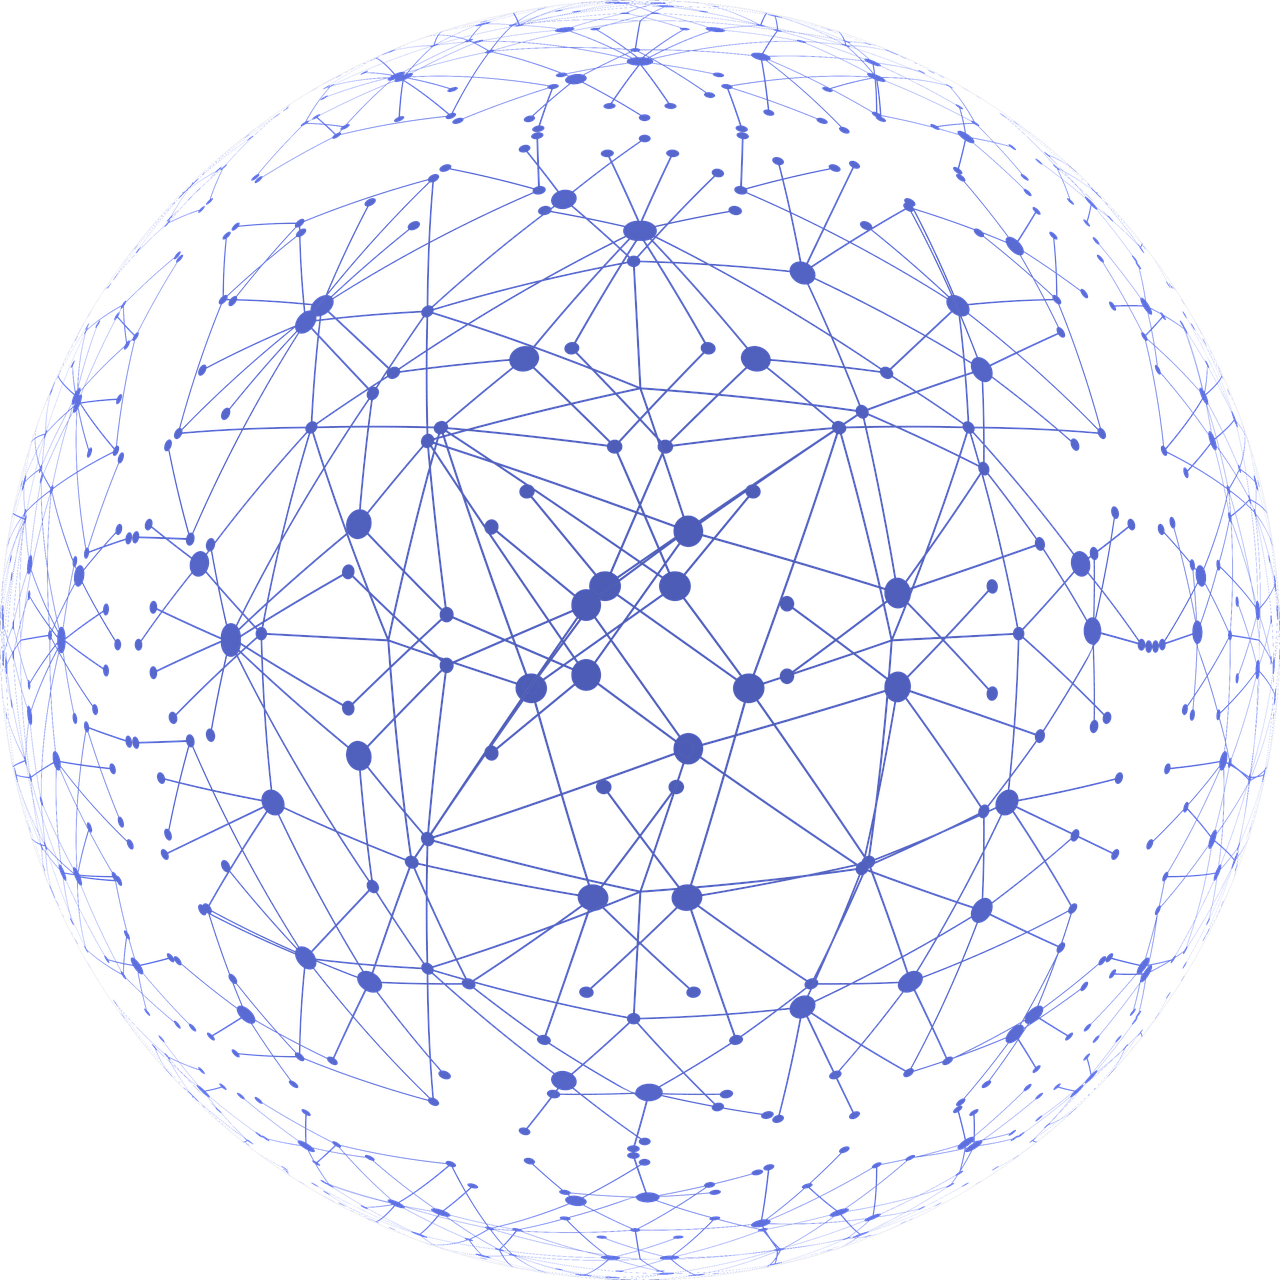
\includegraphics[width=0.3\textwidth]{Kap2/Network.png}
    \caption{Social Network.}
    \label{fig:Social_net}
\end{center}
\end{figure}


% An edge or link represents multiple kinds of relations, depending on the application, e.g., the local position in a network of vehicles in a speedway or transactions between an exchange bank network. Two vertices (vi, vj) are adjacent if exist an edge eij=(i,j)E  between vi and vj. the neighbors of i is denotes by the set N_i

A graph $\mathcal{G} = (\mathcal{V,E,W})$ consists of the joint of three fundamental parts. A set of vertices (or nodes) $\mathcal{V} = \left\{ v_o,v_1, ... v_n \right\}$, A set of edges (or links) $\mathcal{E} \subseteq  \mathcal{V} \times  \mathcal{V} =  \left \{ e_{1,2},e_{2,3},...,e_{i,j} \right \}$ and a weight matrix $\matchal{W}$ defined as:\\

\begin{equation}
\mathcal{W}  = \mathcal{W}_{i,j} \left\{ \begin{array}{cl}
> 0 & if (i;j) \in \mathcal{E}, \\
=0 & if (i;j) \notin  \mathcal{E}.
\end{array} \right.
\end{equation}


\begin{figure}[h]
\begin{center}
    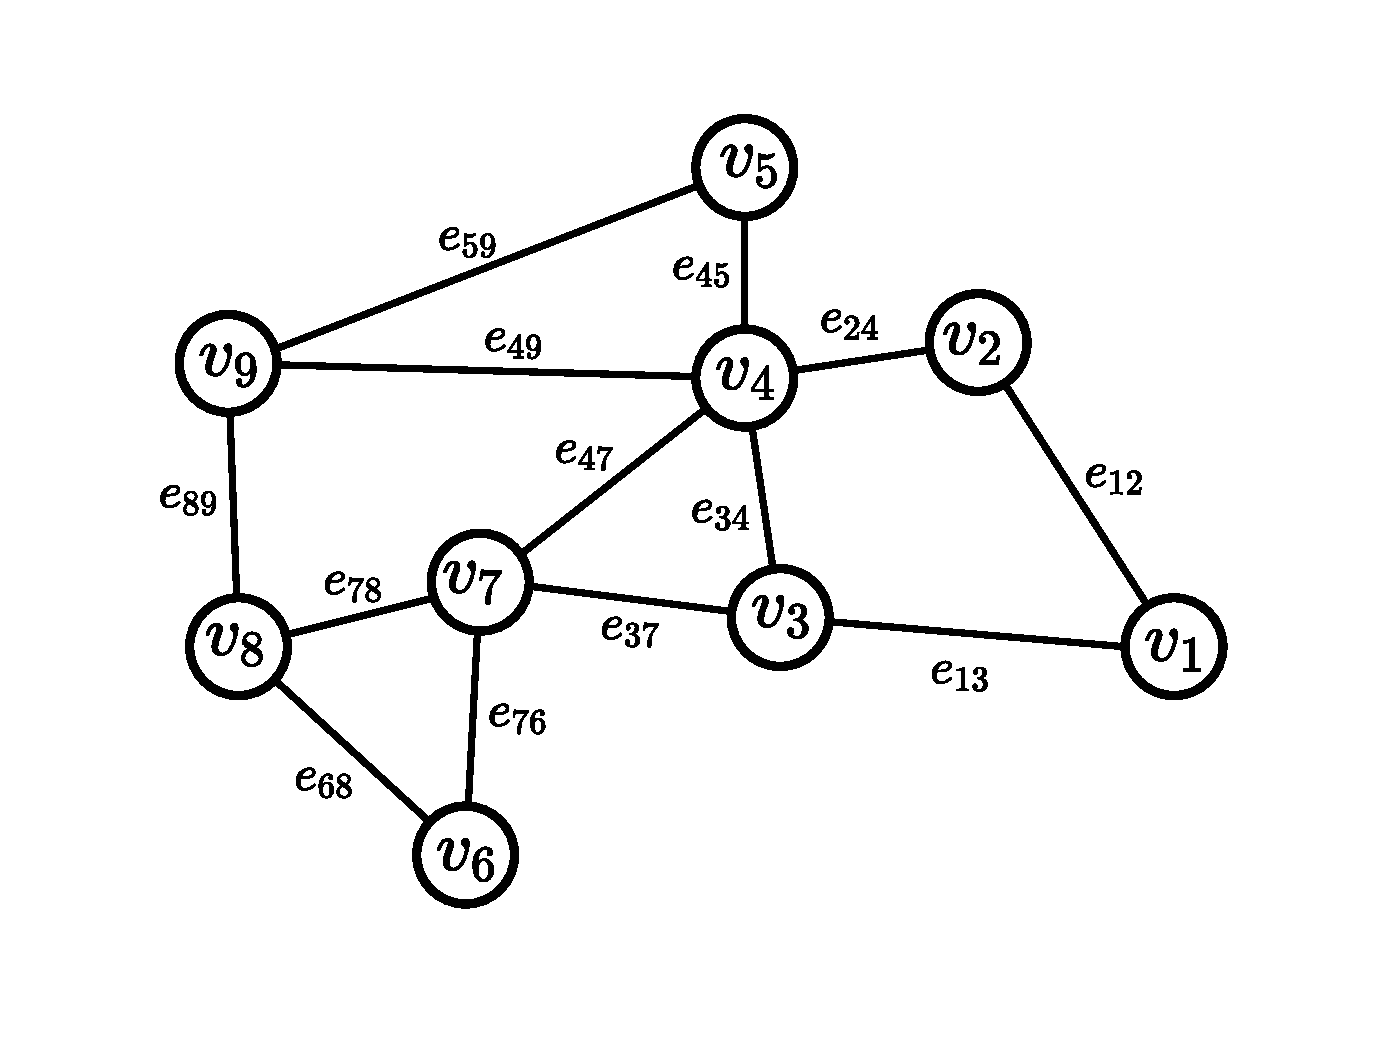
\includegraphics[width=0.7\textwidth]{Kap2/Graph-01.eps}
    \caption{ Graph of Network system.}
    \label{fig:Graph}
\end{center}
\end{figure}


A set of vertices is a group of agents (or nodes) $v = 1,..., n$, where each node is an information source. It could be auto-generated or retransmitted by other nodes. In Fig \ref{fig:Graph} the set of vertices is $\mathcal{V} = \left\{ v_1,v_2,v_3,v_4,v_5,v_6,v_7,v_8,v_9 \right\}$.
However, the edges (or links) are the ways the information is shared. it could be directed or undirected depending on how the information is transmitted if just a node can transmit, or transmit and receive. In the previous example, the set of edges is $ \mathcal{E} = \left\{ e_{12},e_{13},e_{24},e_{34},e_{37},e_{45},e_{47},e_{49},e_{59},e_{68},e_{76},e_{78},e_{89} \right\}$, and lastly the weight matrix is an algebraic representation of the entire interconnected system. If exist a connection between vertice I and j in the matrix, it will be 1; otherwise, it will be 0. In fig \ref{fig:Graph} the weight matrix is:


\begin{equation*}
\centering
\mathcal{W} = \begin{bmatrix}
0 & 1 & 1 & 0 & 0 & 0 & 0 & 0 & 0 \\
1 & 0 & 0 & 1 & 0 & 0 & 0 & 0 & 0 \\
1 & 0 & 0 & 1 & 0 & 0 & 1 & 0 & 0 \\
0 & 1 & 1 & 0 & 1 & 0 & 1 & 0 & 1 \\
0 & 0 & 0 & 1 & 0 & 0 & 0 & 0 & 1 \\
0 & 0 & 0 & 0 & 0 & 0 & 1 & 1 & 0 \\
0 & 0 & 1 & 1 & 0 & 1 & 0 & 1 & 0 \\
0 & 0 & 0 & 0 & 0 & 1 & 1 & 0 & 1 \\
0 & 0 & 0 & 1 & 1 & 0 & 0 & 1 & 0
\end{bmatrix}
\end{equation*}
\\

The neighborhood of node $v_{i}$ is the set of nodes $\mathcal{N}_{i} \subseteq  \mathcal{V}$ that have a direct interaction with agent $i$. This set of edges could be directed or undirected depending on their communication. A graph $\mathcal{G}$ is connected if a connection exists between two or more nodes and there is a route between all nodes in the set $\mathcal{V}$. Finally, the set of nodes of a graph has a degree;  It depends on the number of neighbors of each node. If all graph nodes have the same degree, the graph is called a regular graph.\\

A graph could be represented as a joint of multiple matrices. These matrices show information about each node with the other. 






% ---------------------------- degreee and adjacency --------------------------
\section*{Degree and Adjacency Matrix}

The degree of a node $v_{i}$ is represented as $d(v_{i})$, which is the name of the cardinality of a node, and it represents the number of agents connected with node $i$. Therefore, The degree matrix is a diagonal matrix with the degree values of each node:

\begin{equation}
    \Delta (\mathcal{G}) = \begin{bmatrix}
d(v_{1}) &   0    &  \cdots & 0\\ 
0      & d(v_{2}) & \cdots &  0 \\ 
\vdots & \vdots   & \ddots  & \vdots\\ 
0      & 0        & \cdots & d(v_{n}) 
  \end{bmatrix}
\end{equation}


In addition, an adjacency matrix exists where the relationship of each node with each other is represented. Moreover, the adjacency matrix is defined as:

\begin{equation}
    \left [ Y(\mathcal{G}) \right ]_{ij} = \left\{\begin{matrix}
1, & \text{if } v_{i}v_{j} \in \mathcal{E},\\ 
0, & \text{Otherwise.} 
\end{matrix}\right.
\end{equation}





\section*{Incidence Matrix}
There exist direction or bi-direction graphs in their edges. If a graph exists with directed edges, it is called a digraph $\mathcal{D}$. Therefore, a digraph is described in its incidence matrix, where it represents the orientation of each edge of the graph. This information is useful to evaluate network stability and controllability. This representation is defined as:

\begin{equation}
    I_{ij}(\mathcal{G}) = \left\{\begin{matrix*}[l]
-1, & \text{if } v_{i} \text{ is the tail of } v_{j},\\ 
1, & \text{if } v_{i} \text{ is the head of } v_{j},\\ 
0, &  \text{Otherwise.   }
\end{matrix*}\right.
\end{equation}

A graph could also have weights in its connections, representing the importance of the neighbor's information on each node. If a graph has weighted edges, it is called a weight graph. Consequently, in a weight graph, the adjacency matrix is built by the following definition:


\begin{equation}
    Ad(\mathcal{G}) = \left\{\begin{matrix}
\omega_{ij},   & \text{if } (v_{i}v_{j}) \in \mathcal{E}, \\ 
0, &  \text{Otherwise.}
\end{matrix}\right.
\end{equation}

% ---------------------------- laplacian ----------------------------
\section*{Laplacian}

The Laplacian of a graph is another fundamental representation of a graph. The way of representing a Laplacian graph of a graph $\mathcal{G}$ is by using the joint of adjacency and degree matrix as follows:

\begin{equation}
    L(\mathcal{G}) = \Delta (\mathcal{G}) - Y\mathcal(G)
\end{equation}

Laplacian matrix must be symmetric if it is a digraph or asymmetric otherwise. 










% representacion matricial de grafos

% matriz de grafo y de adyacencia 



% -----------------------------------------------------------------------------


\section{Model Predictive Control}

Model Predictive Control is a control theory used to manage some variables optimally into a function looking at a specific result. The main idea is to use a discrete model of the entire system to predict future system states. With the capability of predicting future behaviors over a finite-time prediction and control horizon $H_u$ and $H_p$, depending on different inputs. It is possible to optimize the input control to achieve an optimal solution. The process is to apply an optimal input signal to the system and recalc the next optimal step. This process is repetitive while the system aims at the principal objective. In the first step, it measures the error of the actual and desired state, and also the amount of energy implemented as shown in Fig  \ref{fig:mpc1}. With this information optimize the states error and control input to achieve its objective Fig \ref{fig:mpc2}. MPC benefits are achieving the main goal while considering some constraints, the ease of design, simulation, and implementation in different systems, and the powerful way to control linear and nonlinear systems. This section describes the mathematical theory of a Model Predictive Control and its applications in the described scenario.


\subsection{Dynamic Prediction Model}

Considering a discrete model system (\ref{eq:mpc2}) and the observably output model (\ref{eq:mpc}), where $x(t) \in \mathbb{R}^n$ represents the state values at time $t$, the $u(t) \in \mathbb{R}^m$ variable as the discrete control input signal at the time $t$. The output is represented as  $y(t) \in \mathbb{R}^p$.

\begin{align}
    x(t+1) = f(x(t),u(t)),\label{eq:mpc2}\\
    y(t) = g(x(t),u(t)). \label{eq:mpc}
\end{align}

The dynamic equation \ref{eq:mpc2} express the evolution  of the states $f:\mathbb{R}^n \times \mathbb{R}^m \to  \mathbb{R}^n$ over the horizon $H_u$ and the output function shows the behavior $g:\mathbb{R}^n \times \mathbb{R}^m \to  \mathbb{R}^p$ over the horizon $H_p$. 
In order to reduce computation load and time delays, a linearized prediction model can be set up using the state evolution in \ref{eq:dynamic} . This thesis document linearized some convex models; however, all dynamic models will be explained in-depth in the next chapter. While the controller is working, this linearization is being processed in each iteration around the actual states. hence, a matrix E is added to the state matrix A and input matrix B. Future states are predicted using the following iterative substitution

\begin{align}
x(t+1) & = Ax(t) + Bu(t)+E \\
x(t+2) & = Ax(t+1) + Bu(t+1)+E\\
       & = A^2x(t) + ABu(t)+AE +Bu(t+1) +E\\
       & \vdots  \\
x(t+H_u) & = A^{H_u}x(t) + A^{H_u-1}Bu(t)+\cdots + Bu(t+H_u-1)+ A^{H_u-1}E+\cdots +E\\
      & \vdots  \\
x(t+H_p) & = A^{H_p}x(t) + A^{H_p-1}Bu(t)+\cdots + Bu(t+H_p-1)+ A^{H_p-1}E+\cdots +E
\label{eq:dynamic}
\end{align}

The resulting system is represented by matrices $A(t) \in \mathbb{R}^{n \times n}, B(t) \in \mathbb{R}^{n \times m}, C(t) \in \mathbb{R}^{p \times n} $ and $E(t) \in \mathbb{R}^{n}$ after linearization. This predicted linear model is used when the dynamic model, constraints, and objective function are nonlinear and the computing system has low resources. If this linearization is avoided, the calc could be slower, and the control system could be unstable


\begin{figure}[H]
\begin{center}
    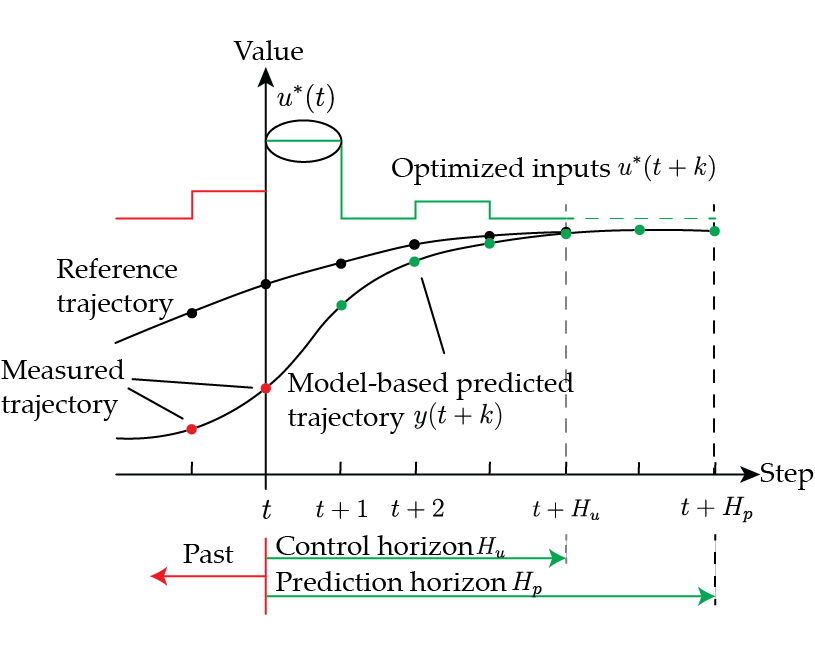
\includegraphics[width=0.57\textwidth]{Kap2/mpc1.png}
    \caption{Control and state signals, First iteration.} 
    \label{fig:mpc1}
\end{center}
\end{figure}

\begin{figure}[H]
\begin{center}
    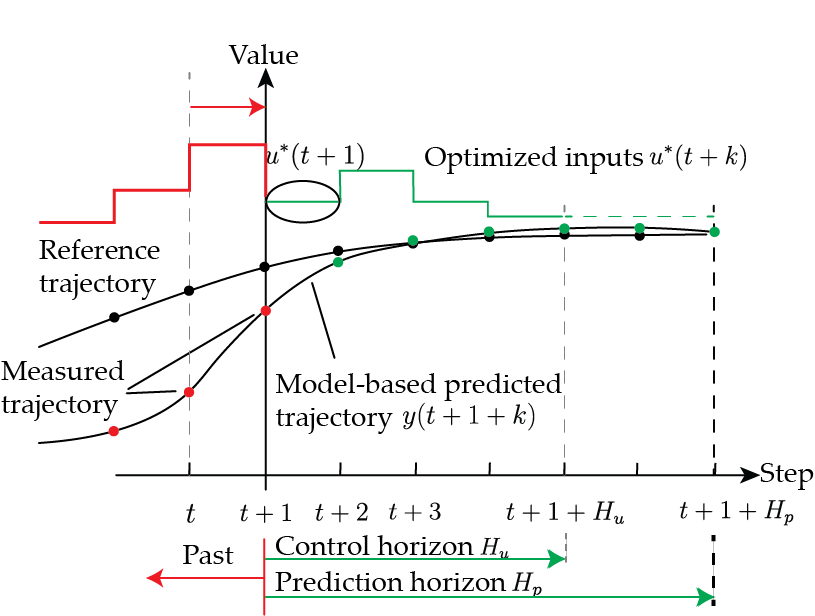
\includegraphics[width=0.57\textwidth]{Kap2/mpc2.png}
    \caption{Control and state signals, Second iteration.}
    \label{fig:mpc2}
\end{center}
\end{figure}




\subsection{Objective Function}

The objective function is the principal function representing the controller's aim needs to be achieved. This function is also called the cost function. Generally, it is divided into two parts: the \textit{Running cost} and \textit{Terminal costs}. The running cost penalizes the difference between the actual and desired states and control inputs. It allows for tracking a reference and optimizing the consumption of energy. The latter penalizes the weighted difference between the final predicted and the final reference step $\tilde{x}(H_p)$. The objective function is defined as:

\begin{equation}
    V(\tilde{x},\tilde{u})= \underbrace{\sum_{k=1}^{H_p-1} \tilde{x}(k)^T Q_i \tilde{x}(k) +\sum_{k=1}^{H_u-1} \tilde{u}(k)^T R_i \tilde{u}(k)}_\text{Running cost} + \underbrace{\tilde{x}(H_p)^T P \tilde{x}(H_p)}_\text{Terminal cost}.
    \label{eq:obj_func}
\end{equation}

Using \ref{eq:dynamic} and replacing in \ref{eq:obj_func}, the objective function is now:


\begin{equation}
    V(\tilde{x},\tilde{u})= \tilde{x}^T Q \tilde{x} +\tilde{u}^T R \tilde{u}.
    \label{eq:V_matrix}
\end{equation}

The terminal cost is augmented in the running cost using the subsequent definitions. The weight matrix $Q$ is represented using $\tilde{Q} = diag(Q_1,\cdots, Q_{H_p-1},P)$, and $Q_{i}, P \in \mathbb{R}^{n \tiomes n}$ and $R \in \mathbb{R}^m$. The evolution of the states over the horizon $H_p$ and $H_u$ are denoted by the matrices $\tilde{x}$ and $\tilde{u}$ as follows: 


\begin{equation}
    \tilde{x} = \begin{bmatrix}
x(1) - x_ref(1)\\ 
x(2) - x_ref(2)\\ 
\vdots  \\ 
x(H_p)-X_{ref}(H_p)
\end{bmatrix},
\tilde{u} = \begin{bmatrix}
u(1) - u_ref(1)\\ 
u(2) - u_ref(2)\\ 
\vdots  \\ 
u(H_u)-u_{ref}(H_u)
\end{bmatrix}.
\end{equation}


If the MPC is linearized, the number of variables to optimize will decrease, redefining \ref{eq:V_matrix}. This function only will depend on the control inputs variables. It will convert the convex function into a Quadratic Problem (QP), where the variable to optimize is the sequence of the predicted inputs. The optimization problems become as:

\begin{align}
\min_{U_{H_u}} & \quad J \\
s.t. & \ Au \le b, \\
:= \min_{U_{H_u}} & \quad \frac{1}{2}u^T_{H_u}Pu_{H_u} =\frac{1}{2}Qu_{H_u} + r_0 \\
s.t. & \ Au_{H_u} \le  b.
\label{eq:min}
\end{align}


Each term in \ref{eq:min} is defines as \ref{eq:P_matrix}

\begin{equation}
    u_{H_u} = \begin{bmatrix}
u(1) \\
u(2) \\
\vdots  \\
u(H_u-1)
\end{bmatrix}, P=S^T\tilde{A}S + R, q=\left[ x(k)^T \tilde{x}^T_{H_p} \tilde{u}_{H_u}\right]
\begin{bmatrix}
S^T \tilde{Q}T \\
QS \\
R
\end{bmatrix},
\label{eq:P_matrix}
\end{equation}

$T$ and $S$ are denoted by:

\begin{equation}
T = \begin{bmatrix}
I \\
A \\
A^2 \\
\vdots  \\
A^N
\end{bmatrix},
S= \begin{bmatrix}
0 & 0 & \cdots  & \cdots & \cdots & 0 \\
B & \ddots  &  &  &  &  \\
AB & \ddots & \ddots &  &  &  \\
A^B & \ddots & \ddots & \ddots &  &  \\
\vdots & \ddots & \ddots & \ddots & \ddots & 0 \\
A^{N-1}B & \cdots & A^2B & AB & B & 0
\end{bmatrix}.
\end{equation}

% ---------------- constraints

\subsection{Constraints}


One of the advantages of MPC is the good handly management of constraints. the following are the benefits of the use of an MPC controller with constraints
\begin{itemize}
    \item States, inputs, and dynamic model systems can implement constraints ensuring safety control.
    \item The use of constraints can guarantee stability and robustness to the whole system.
    \item The MPC design could constraint the control input to ensure physical limitations on actuators. however, the output or the system also could be constrained to represent a limitation on the agent.
\end{itemize}
\\
The input, state, and output variables are constrained, limiting the workspace across their prediction horizon. On the whole, constraints result are represented as:

\begin{align}
x(t+k) & \in \mathcal{X} \subseteq \mathbb{R}^n, k=1,\cdots,H_p, \\
y(t+k) & \in \mathcal{Y} \subseteq \mathbb{R}^p,\  k=1,\cdots,H_p, \\
u(t+k) & \in \mathcal{U} \subseteq \mathbb{R}^m, k=0,\cdots,H_u-1.
\end{align}


\section{Alternate Direction Method of Multipliers}
% //////////// GAME THEORY ////////////
\section{Game Theory}

\begin{figure}[H]
\begin{center}
    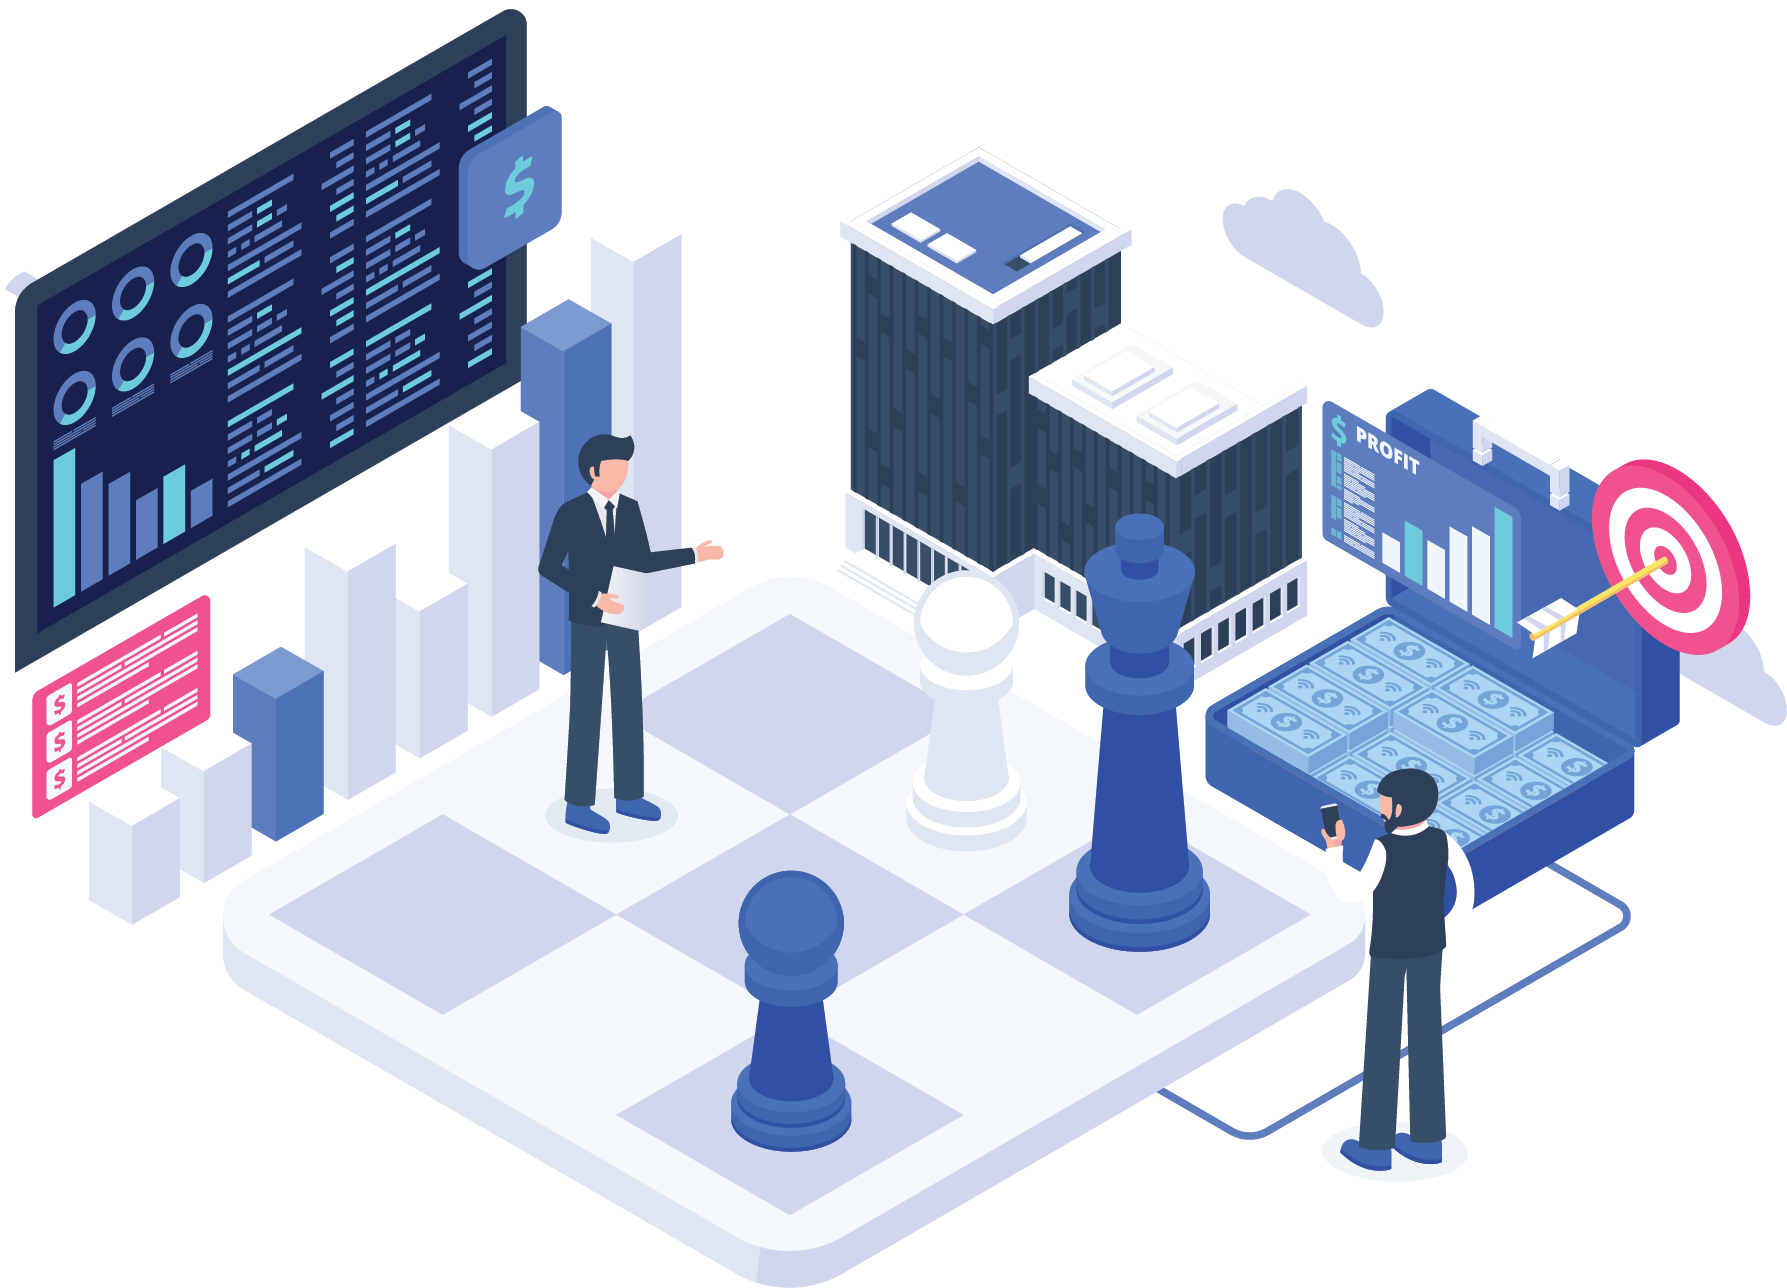
\includegraphics[width=0.57\textwidth]{Kap2/Strategy.png}
    \caption{Strategy in economics environment.}
    \label{fig:game_theory}
\end{center}
\end{figure}

Game theory is a mathematical method mainly used to analyze and achieve the best decision in a multi-agent environment. It is highly used in cooperative or competitive games. Nobel price John Nash originates it in \cite{nash_novel}, which establishes the basis of this novel theory.
Nash developed the theory to be implemented in social sciences and economics fields. The general idea in economics is to take decisions on a market, taking into account the decision of the other agents can affect the price of some commodity, and a company or agent has to take action to achieve the desired goal Fig. \ref{fig:game_theory}. Eventually, this theory has proven in fields such as engineering, computer science, philosophy, and many other fields,\cite{33t_GameTheory2}, \cite{46t_inproceedings}, obtaining good results. 

From a control theory perspective is possible to interpret game theory law as a sort of "intelligent rational decision-maker" \cite{Marden2018}. In other words, game theory is the study and control of conflict and cooperation between interacting controllers, where the success depends on the agents, the preferences, and the settings.
One setting is a zero-sum game, where more than one player exists, and the profit of one player is the detriment of the other ones. That is, the sum of the profits is zero. It is common to use this setting where the game has limited resources, and the objective of each agent is the same.
Another setting is team games. In this setting, a group of agents looks for a cooperative strategy to achieve the global objective. Commonly, this kind of game's architecture is decentralized, and each agent has the same objective.
The third setting is where agents do not work cooperatively. Each agent tries to achieve a local objective in an environment depending on the neighbors' decisions, but each agent has a different objective. This kind of setting is usually decentralized and non-cooperative.


This section gives a simple example of a discrete matrix game before explaining the elements of a game theory in a continuous space. Finally, it is explained the third setting as potential games specifically. All information explained in this section is obtained from \cite{18t_article}, \cite{19t_article}, \cite{20t_article}, \cite{29t_book}, \cite{30t_phdthesis}, \cite{46t_inproceedings}.



The discrete matrix form is the most simple and powerful representation of the perspective and profit of each agent. A game written in matrix form shows all possible decisions of an agent and its corresponding utility or cost. Next is explaining one of the most popular examples of matrix games.

% ------------------------------------------------------
\subsection{Game Theory Example: Prisoner's dilemma}

Two criminal of a gang has been arrested and imprisoned. Each prisoner is in separate rooms, and no one knows about his couple. Police admit they do not have enough evidence to sentence these criminals to jail. They plan an strategy to get one of them to give enough information to solve the case. The strategy is to inform them that both will be sentenced to a year of prison for the lesser charge. Simultaneously, the police offer each prisoner a bargain. If one testifies against his partner, he will go free while the other one will be three years in prison on the main charge. However, if both prisoners testify against each other, both will be sentenced to two years of prison. Each criminal (agent) has to take a decision depending on the possible decision of the other one. In matrix form, the prisoner's dilemma game is: 


\begin{table}[h!]
\centering
\begin{tabular}{l|l|l}
                                    & \textbf{B refuses deal} & \textbf{B testify against  his pair} \\ \hline
\textbf{A refuses deal}             & 1 year, 1 year          & 3 years, 0 years                     \\ \hline
\textbf{A testify against his pair} & 0 years, 3 years        & 2 years, 2 years                    
\end{tabular}
\end{table}

In the previous example, it is clear that the action of each prisoner would depend on the action of the other prisoner. In a game, each agent looks at its self-interest. by this, a set of interconnected agents in a game with knowledge of other's decisions, and its self profit for each possible decision, can make optimal decisions to look its interest. Game theory helps to formulate this kind of problem in a mathematical manner.


% ------------------------------------------------------
\subsection{Basic Concepts}
\\
we begin with a basic overview. Currently exist many texts explaining this in-depth, including economics (\cite{33t_GameTheory2}, \cite{5shamma_game}, \cite{6shamma_course}), computer science (\cite{7shamma_prediction}, \cite{29t_book}, \cite{9shamma_algorithmic}), and engineering (\cite{10shamma_dynamic}, \cite{11shamma_game},\cite{12shamma_noncooperative}).

% ------------------------------------------------------
\subsubsection{Game elements:}

A game is fundamentally defined by three elements. First is the \textbf{set of players}, $\mathcal{P}$. For the purpose of this thesis work, we limit the discussion to a finite set of players, i.e., 

\begin{equation*}
\mathcal{P}= \left\{ 1,2,..., N \right\}.
\end{equation*}

Second, for each player $p \in \mathcal{P}$ there is a \textbf{set of strategy}, $\mathcal{S}_p$. The strategy set is 

\begin{equation*}
\mathcal{S} = \mathcal{S}_1 \times ... \times \mathcal{S}_p.
\end{equation*}

a joint strategy set $s \in \mathcal{S}$ is represented as 

\begin{equation*}
s = (s_1,s_2,...,s_p)
\end{equation*}

Also, the notation $s_{-p}$ denotes the set of strategies of players $\mathcal{P} \backslash p$, i.e., players other than player $p$. Finally, for each player $p \in \matchal{P}$, there is a utility function 

\begin{equation*}
u_p : \mathcal{S} \to \mathbb{R}
\end{equation*}

This function expresses the player's preferences over the strategies. For any two joint strategies, $s, \acute{s} \in \mathcal{S}$, player $p$ prefers $s$ to $\acute{s}$ if and only if

\begin{equation*}
 u_p(s) > u_p(\acute{s}).
\end{equation*}

In utility functions, bigger number is better. In case of $u_p(s) = u_p(\acute{s})$, the player $p$ will be indifferent between which strategy to choose. The \textbf{vector utility function} is denoted by $u$, i.e.,

\begin{equation*}
u = (u_1, u_2, ..., u_p) : \mathcal{S} \to \mathbb{R}^P.
\end{equation*}

Sometimes, it is better to express a game in terms of cost functions rather than utility functions. In this case, a small number is better. For each player $p \in \mathcal{P}$, there is a cost function 

\begin{equation*}
c_p : \mathcal{S} \to \mathbb{R}
\end{equation*}

and player $p$ will prefer the joint strategy $s$ over $\acute{s}$ if and only if, 

\begin{equation*}
c_p(s) < c_p(\acute{s}).
\end{equation*}

A general game can be represented by an optimization problems: 

\begin{equation}
    \forall i \in P = \left\{ 1,2,..., N \right\}, \ \min_{s_i \in \mathcal{S}_i} c_p(s_i, \textbf{s}_{-i})
\end{equation}

Where the solution to this optimization problem (OP) is called Nash Equilibrium (NE). To get more knowledge of Nash equilibrium problems, we will look at games from each agent's point of view. If an agent has information about the other agents' strategy, his problem becomes simple. Specifically, he would have to solve a problem of a unique agent, where the main task is to choose the best action to get the best utility or minimum cost. However, if agents $-i$ were to commit to playing $s_{-1}$, the agent $i$ would face the problem of choosing the best response depending on the possible decision of the other agents.

% ------------------------------------------------------
\subsubsection{Best Response}

The best response of the player $i$ to the set of strategy $s_{-i}$ is a mixed strategy $x_i^{*}$ such as 

\begin{equation*}
c_p(s_i^*, s_{-i}) < c_p(s_i, s_{-i}),
\end{equation*}
 
for all strategies $ s_i \in \mathcal{S}$. \\

Looking at the example of the prisoner dilemma. Suppose one prisoner knows that the other prisoner will refuse the deal. His best response is turning state's evidence. The best response is not unique, and it is not a solution concept. However, it helps to understand arguably the most crucial notion in game theory, the Nash equilibrium.
The best response function $BR_p : \mathcal{S}_{-p} \to 2^{\mathcal{S}_p}$ is defined by 

\begin{equation*}
    BR_p(s_{-p}) : \left\{ s_p \in \mathcal{S}_{p} : u_p(s_{p},s_{-p}) \ge u_p(\acute{s_{p}},s_{-p}) \text{ for all } \acute{s_{p}} \in \mathcal{S}_{p} \right\} .
\end{equation*}

$BR_p(S_{-p})$ is the set of strategies where the maximum utility of the player p in response to the other strategies $s_{-p}$ is achieved. Note that it does not need to be unique and could have multiple best responses.


\subsection{Nash Equilibrium}


At Nash equilibrium, each player's strategy is optimal concerning the other players' strategies. In words, the set of strategies $(s_1^*,s_1^*, ... ,s_P^*) \in \mathcal{S}$ is a Nash equilibrium, if for each $p$ exist a strategy that accomplish 

\begin{equation*}
    s_p^* \in BR_p(s^*_{-p})
\end{equation*}


\subsubsection{Example Nash equilibrium}
Two players in a game have one decision variable $(x,y)$ respectively; that means $n_1=n_2=1$. Each decision variable $x \in \mathbb{R}$ and $y \in \mathbb{R}$ denote the player's strategies.
The game problem is represented as 

\begin{equation}
\begin{matrix}
\min_y \quad y^2 + xy & \ & \qquad & \min_x \quad (y-x)^2 \\
s.t.: -1 \le  y \le 1 & \ & \qquad & s.t.: 0 \le  x \le 1
\end{matrix},
\end{equation}

solving this optimization problem we get the optimal solution:

\begin{equation}
\begin{matrix}
\mathcal{S}_1(x) = \left\{ \begin{array}{cl}
1 & : \ x  < -2 \\
-x/2 & : \ -2 \leq x \leq 2 \\
-1 & : \ x > 2
\end{array} \right. 

& &

\mathcal{S}_2(y) = \left\{ \begin{array}{cl}
0 & : \ y  < 0 \\
y & : \ 0 \leq y \leq 1 \\
1 & : \ y > 1
\end{array} \right.
\end{matrix}.
\end{equation}



\subsubsection{$\epsilon$-Nash Equilibrium}

\subsection{Generalized Nash Equilibrium Problems}


\subsection{Generalized Potential Games}



\chapter{Problem Statement}

From the beginning of civilization, humans have been looking to transport from one place to another more efficiently than walking. First, they started with horses and floats, but horses had a brain and could make their own decisions; sometimes, those decisions were based on an emotional reaction rather than intelligent choices. Moreover, it could not continuously work for a long duty cycle, and its power was limited. Later in 1769, Nicolas-Joseph Cugnot invented the first steam-powered vehicle. This incredible machine could load an extended weight, and drivers could make their own driving decisions. Until now, this transportation system is still working, unless the advantage of efficiency, power consumption, pollution, and safety is not enough to be an optimal way to transport people and loads.\\

Research areas have made many efforts to achieve an optimal way of transportation to be accessible, optimal, and safe for everybody. Some ideas have been proposed, like hydrogen, diesel, and natural gas engines. Also, some Nobel research about control safety systems like better and more powerful breaks, automated airbags, and good chassis material tries to save more lives, but it is not enough. Unfortunately, all past advantages are focused on the driver and vehicle users. Currently, no control system guarantees the security and integrity of the other road authors. The human decision in a driving context frequently represents a danger because it is based on emotion and natural reactions making no optimal driving. Even though these options could improve the current vehicles, they may find a better and cheapest solution to the main problem.\\

The research areas try to solve the safety driving problem with deep learning, Recurrent Neural Networks, machine learning, and other theories. However, using these theories only guarantees stability and controllability in some scenarios. To get a closer solution to this problem, we study one way of achieving security and efficiency in a particular method as a highway area in this thesis work. Currently, the experts on optimal control system areas rely on automated driving. This technology could solve all of the problems mentioned above.\\

Some safety decision criteria that we take into account were the following:
\begin{itemize}
\item Avoid obstacles that may be on the road.
\item Avoid a collision with other cars on the road regardless of whether it is a cooperative or non-cooperative agent.
\item Make decisions in the presence of aggressive maneuvers by selfish or non-cooperative agents on the road.

\end{itemize}


Therefore, designing and implementing different controllers with access to specific data sets was necessary. It depends on each controller's necessity. These decisions are based on logical and optimal decision-maker control to achieve the desired goal.

 These decisions are based on safety rules established for the users of any particular road.


% --------------------- automated driving --------------------
\section{Automated driving}
The idea of automated driving is to safely and efficiently coordinate and synchronize several autonomous vehicles (AV) safely and efficiently.\\

Managing many AVs requires an extensive network with high computational loads and advanced control techniques. Usually, in the research literature is implemented one control algorithm is for an agent to achieve the objective. However, automated driving is an area that must consider different scenarios and situations. Besides, it is essential to prove all possibilities for warranty security and controllability. This thesis studies some control theories and the best state to implement.

\begin{itemize}
    \item  \textbf{Mixed-Integer Potential Game:} uses integer and continuous variables in a cost function to control the AV's position and velocity on a highway optimally.
    \item  \textbf{Model Predictive Control:} uses information about the environment and local variables to get the optimal decision avoiding near obstacles.
    \item  \textbf{Alternating Direction Method of Multipliers:} utilize a linear model of the AV and inequality constraints as possible to get a faster and more efficient solution to the problem. 
\end{itemize}

All the above controllers are explained in detail in chapter 4. In addition, the following section describes how AV and collision avoidance are modeled. 






% -----------------------------------------
\section{Vehicle Model}

The automated driving task is complex, and one model is not enough to represent the behaviour of a vehicle around the environment. However, multiple controllers require multiple models that give the correct information. We use three different controllers that have a specific task. Each of them needs a particular model of vehicle. The high-level controller takes the network's information. For that reason, we implement a linear model. The middle-level controller uses just the knowledge of the environment acquired by its sensors. Due to this reason, we implemented a unicycle model. Besides, the low-level control gets information about the car and its decision-making behavior. Thus, we use a differential model in this control section. 


% -----------------------------------------
\subsection{Linear Model System}
\label{linear_model_system}

For controllers based on game theory, convexity is the main prerequisite for convergence. Therefore, the robot model and its constraints must be linear and convex. Due to this, the system is based on a Mixed-Logical-Dynamical system \cite{BEMPORAD1999407}. We consider a set of vehicles $\mathcal{I}:= \left \{ 1, ..., N \right \}$ where N is the total number of vehicles interacting with the local agent in a multi-lane environment. The set  $\mathcal{L}:= \left \{ 1, ..., L \right \}$ represents the set of current lines on the highway, and the L variable is the maximum number of lines on the way. We assume that each vehicle $i$ can control its longitudinal speed $v_i \in \mathcal{V}_i \subset \mathbb{R}$  and can change lane $z_i \in \mathcal{L} \subset \mathbb{N}$. Over the prediction horizon $\mathcal{T} := \left \{ 0, ... ,T \right \} , T\geq 1$. We use two different decision variables to better represent an AV on a highway. Mixed logical variables can simplify, make linear, and convex the entire system. 

\begin{figure}[H]
    \centering
    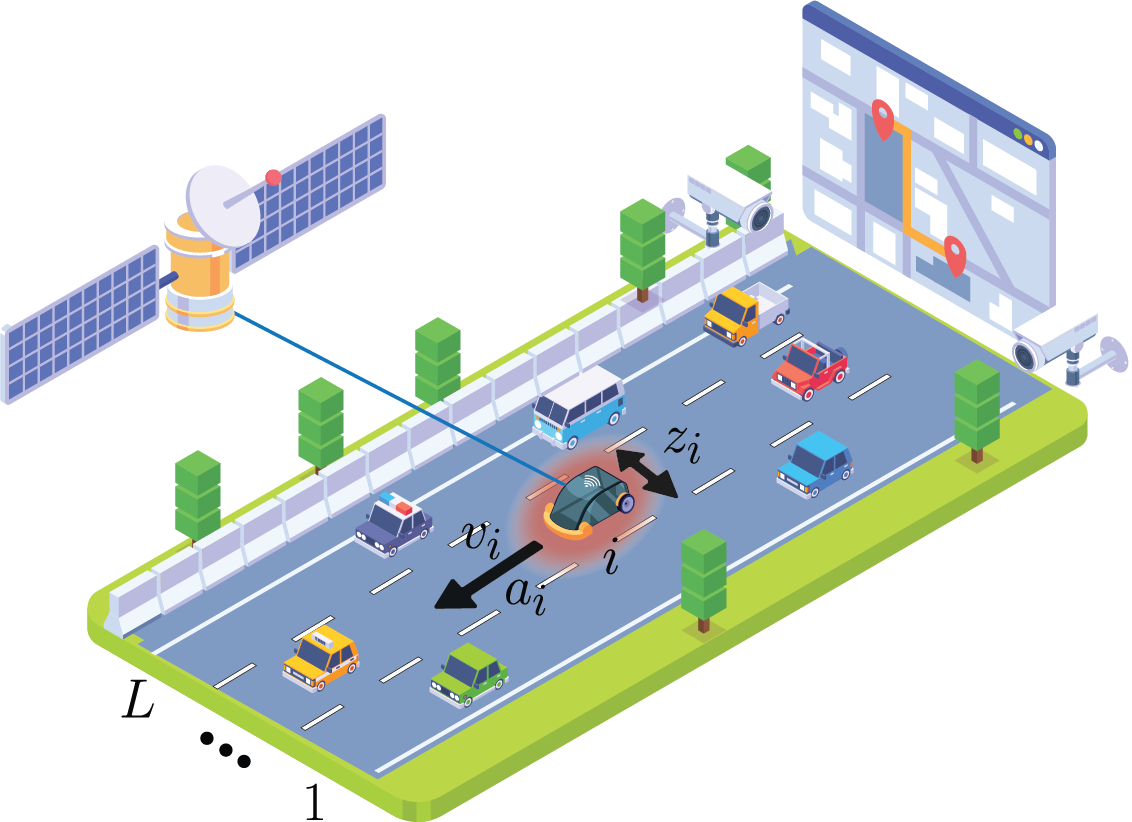
\includegraphics[width=0.8\textwidth]{Kap3/linear_model.png}
    \caption{Linear model's variables.}
    \label{fig:variables}
\end{figure}


\subsubsection{Continuous Decision Variables}
\label{continous_decision_variables}

Each vehicle model has continues variables that represent some physical features. Longitudinal acceleration $a_i \in A_i := \left [ \underline{a_i}, \overline{a_i} \right ] \subset \mathbb{R}$, the variables $\left \{ \underline{a_i}, \overline{a_i} \right \}
$ represent the minimum and maximum acceleration allowed, with $\underline{a_i}< 0 <  \overline{a_i} $, assuming that the $\underline{a_i}$ is negative and is due the break job of the $i$ vehicle, as illustrated in Fig. \label{fig:variables}. The longitudinal speed $v_i \in \mathcal{V}_i \subset \mathbb{R}$ is determined by a standard Forward-Euler Scheme, i.e.,

\begin{gather}
v_i(t+1) = v_i(t) + \tau a_i(t),
\end{gather}

where $\tau > 0$ denotes the time interval of each simulation step. Hence, the acceleration and velocity longitudinal over the horizon $\mathcal{T}$ are: 
\begin{gather*}
a_i := \left [ a_i(0); ...; a_i(t-1) \right ] \in \mathcal{A}^T_i, \\
v_i := \left [ v_i(0); ...; v_i(t-1) \right ] \in \mathcal{V}^T_i
\end{gather*}




\subsubsection{Discrete Decision Variables}
\label{discrete_decision_variables}
The lanes in a highway are predefined internationally as a space where vehicles can and should travel. Thanks to this design, the agent will drive inside a lane unless the vehicle needs to change to another one. That means the set of vehicles $\mathcal{V}$ needs to be modelled as an integer variable that represents the actual and future travelling lane $z_i \in \mathcal{L}$. The discrete decision variables over the horizon $\matchal{T}$ are:

\begin{gather*}
z_i := \left [ z_i(0); ...; \ z_i(t-1) \right ] \in \mathcal{Z}^T_i.
\end{gather*}



\subsubsection{Coupling Variables}



The control system requires different sense variables that allow knowing the actual and future states of the agent $i$ with its neighbours $\mathcal{I}_{-i}$. Therefore, we denote by $d_{i,j} \in \mathbb{R}$ as the longitudinal distance between the connected vehicles $i$ and $j$ at the time $t \in \mathcal{L}$ as shown the Fig. \ref{fig:distance}. 



\begin{figure}[H]
    \centering
    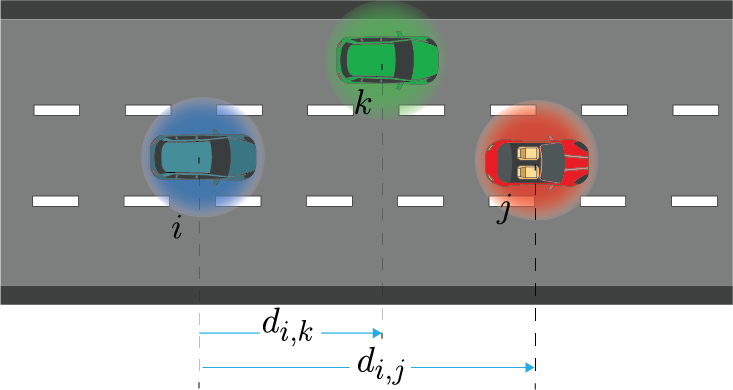
\includegraphics[width=0.7\textwidth]{Kap3/Asset 4.png}
    \caption{Relative distance between agents.}
    \label{fig:distance}
\end{figure}


Over time, the equation of $d_{i,j}$ evolves as a Forward-Euler function. In Eq. \ref{eq:distance} the longitudinal distance is over the axis $x$ in the working environment. The difference in distance velocities is over the current time $t$, and the $\tau$  delta time is the controller's step time for each iteration.

\begin{equation}
d_{i,j}(t+1)= d_{i,j}(t) + \tau(v_j(t)-v_i(t)).
\label{eq:distance}
\end{equation}



It allows us to introduce the set of vehicles in the neighbourhood of  $\mathcal{N}_i:= \left\{ j \in \mathcal{I}  | \left| d_{i,j} \right| \le \overline{d}, t \in \mathcal{T}\right\}$; this data can be measured locally or globally example, on the on-board sensors or with communication of a driving network. From now we refer to the variable $j$ as a generic vehicle in the set $\mathcal{N}_i$. According to \label{eq:distance}, each agent knowing the velocity of its neighbour $v_j(t)$, can estimate the relative distance between each other.
In addition, we implement a relative lane distance $z_{i,j}$. It represents the lateral distance of each vehicle from its neighbours. The difference of lane between agent $i$ with its neighbors $\mathcal{N}_i$ and is calculated by the following equation:



\begin{equation}
z_{i,j}(t)= z_{j}(t) - z_{i}(t).
\label{eq:lanes}
\end{equation}



Lateral distance is the difference between integer values. It means the space working is $\mathbf{N} \times \mathbf{N} \to \mathbf{N}$. The distance is calculated over the $y$ axis.


\begin{figure}[H]
    \centering
    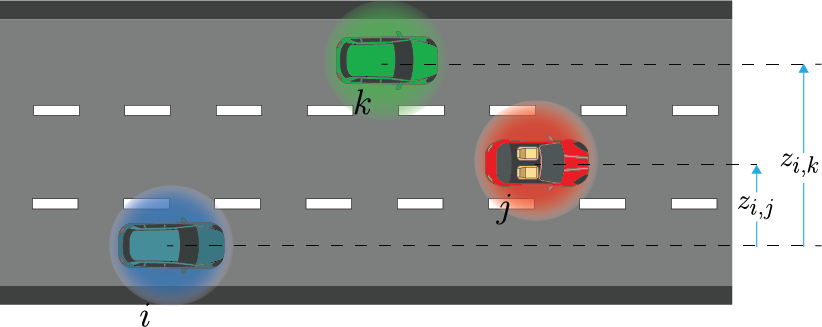
\includegraphics[width=0.8\textwidth]{Kap3/Asset 5.png}
    \caption{Lateral Distance.}
    \label{fig:lanes}
\end{figure}

We assume that each agent makes decisions for their selfish interest, e.g., drive through desired speed profile $v_i^d \in \mathcal{V}^T_i$ or get into a lane $z_i^d \in \mathcal{L}^T_i $. Each agent's control system takes into account its neighbours' current and future state. Still, it does not provide information about the targets of the other agents. As a result of this behaviour, each agent takes a decision seeking its individual goals through a sequence of hybrid decisions.
With the previous model, we formulate as a first step a Model Predictive Control (MPC) motion planning with mixed-integer variables:

\begin{align}
\left\{ \begin{matrix}
\begin{aligned}
 \min_{v_i, a_i, z_i} & J_i(v_i, a_i, z_i) & \\
\text{s.t.} \quad & v_i(t+1)=v_i(t)+ \tau \ a_i(t), & \forall t \in \mathcal{T} \\
& a_i(t) \in \mathcal{A}_i,  &   \\
 & v_i(t+1) \in \mathcal{V}_i,  &   \\
 & z_i(t+1) \in \mathcal{L}_i,  &   \\
\end{aligned}
\end{matrix} \right.
\label{eq:MPC1}
\end{align}


% \begin{align}
% \left\{\begin{matrix}
% \begin{aligned}
% \min_{v,a,z, l_i^l,l_i^r} \quad & J_i\left ( v_i, a_i, z_i \right )\\
% \textrm{s.t.} \quad & v_i(t+1) = v_i(t)+\tau a_i(t), & \forall t \in \mathcal{T}\\
%   &   z_i(t+1) = z_i(t) + l_i^l(t) - l_i^r(t),  & \forall t \in \mathcal{T} \\
% & a_i(t) \in \mathcal{A} , & \forall t \in \mathcal{T} \\
% & v_i(t) \in \mathcal{V_i} , & \forall t \in \mathcal{T} \\
% & a_i(z) \in \mathcal{L_i} , & \forall t \in \mathcal{T} \\
% &  l_i^l(t),l_i^r(t)\in \mathbb{B},  & \forall t \in \mathcal{T} \\
% & l_i^l(t) + l_i^r(t)  \leq 1, & \forall t \in \mathcal{T}\\
% & (\text{\ref{eq:4_6real}}) - (\text{\ref{eq:4_20}}) . & \forall j \in \mathcal{N}_i, \forall t \in \mathcal{T} 
% \end{aligned}
% \end{matrix}\right.
% \label{eq:MPC_problem}
% \end{align}


\\
The $J_i$ cost function is a linear and convex objective for each vehicle $i$ where $J_i:\mathcal{V}^T_i \times \mathcal{A}^T_i \times  \mathcal{L}^T_i \longrightarrow  \mathbb{R}$. The sets $\mathcal{V}_i$ and $\mathcal{L}_i \subset \mathcal{L}$ shall be defined to restrict them to possible values in the real environment. Given maximum and minimum acceleration $\left[ \underline{a_i}, \overline{a_i} \right]$ as also maximum and minimum Velocity $\left[ \underline{v_i}, \overline{v_i} \right]$, we can limit the sets as:

\begin{align}
    \mathcal{V}_i(t) & :=\left[ 0,\overline{v_i(t)} \right] \cap \left[ v_i(t)+ \tau  \underline{a_i},\quad v_i(t)+ \tau  \overline{a_i} \right]
    \label{eq:set_v}
\\
    \mathcal{L}_i(t) & :=\mathcal{L} \cap \left[ z_i(t) -1, \quad z_i(t)+1 \right]
    \label{eq:set_z}
\end{align}

From \ref{eq:set_v}, it is possible to limit the speed to legally possible values, and from \ref{eq:set_z} limits the change of lane to just one per step. This restriction makes agents' movement smoother through lanes and allows lateral safety rules. The following section explains the rules to make safer automated driving with selfish agents.

\subsubsection{Collision Avoidance Rules}
 
Human driving is usually unsafe; exist some rules established in each country, like speed limits, preferential lanes, and safety distance. In this section, we postulate some safety rules to avoid the collisions of the interconnected agents with the presence of non-cooperative agents.\\

% -----------------------------------------------------------------------------
\subsubsection{Longitudinal rules}
The main reason for a collision of two or more vehicles is that one of the vehicles violates the safety distance. Due to this is implemented the following safety rule. If the lateral distance between two agents is equal to zero $z_j(t)=z_i(t) $ and the longitudinal distance is greater or less than a safety distance $\left| d_{i,j}(t) \right| > D_s$, and the agents will continue in the same lane $z_i(t+1) =  z_i(t), z_j(t+1) =  z_j(t)$. The control system must ensure that the behind vehicle maintains a safety distance $\left| d_{i,j}(t) \right| > D_s$ how is shown in Algorithm \ref{alg:safety}, where $D_s$ is a predefined secure distance.\\

\begin{algorithm}
\caption{Algorithm of longitudinal distance}\label{alg:safety}
\begin{algorithmic}
% \FOR $i \in \mathcal{V}$
% \FOR \forall {$i \in \mathcal{V}$} 
\If{$z_{i,j}(t)=0$ and $z_{i,j}(t+1) =0$}
    \If{$d_{i,j}(t) > 0 $}
        \State $d_j(v_j(t)) -d_i(v_i(t)) > D_s$
    \ElsIf{ $d_{i,j}(t) < 0$} 
        \State $d_j(v_j(t)) -d_i(v_i(t)) < -D_s$
    \Else
        
        \State Continue normal driving
    \EndIf
\EndIf

\end{algorithmic}
\end{algorithm}

% ----------------------------------------------------------------------------
\subsubsection{Lateral rules}

\begin{figure}
\begin{subfigure}[H]{1\textwidth}
\centering
    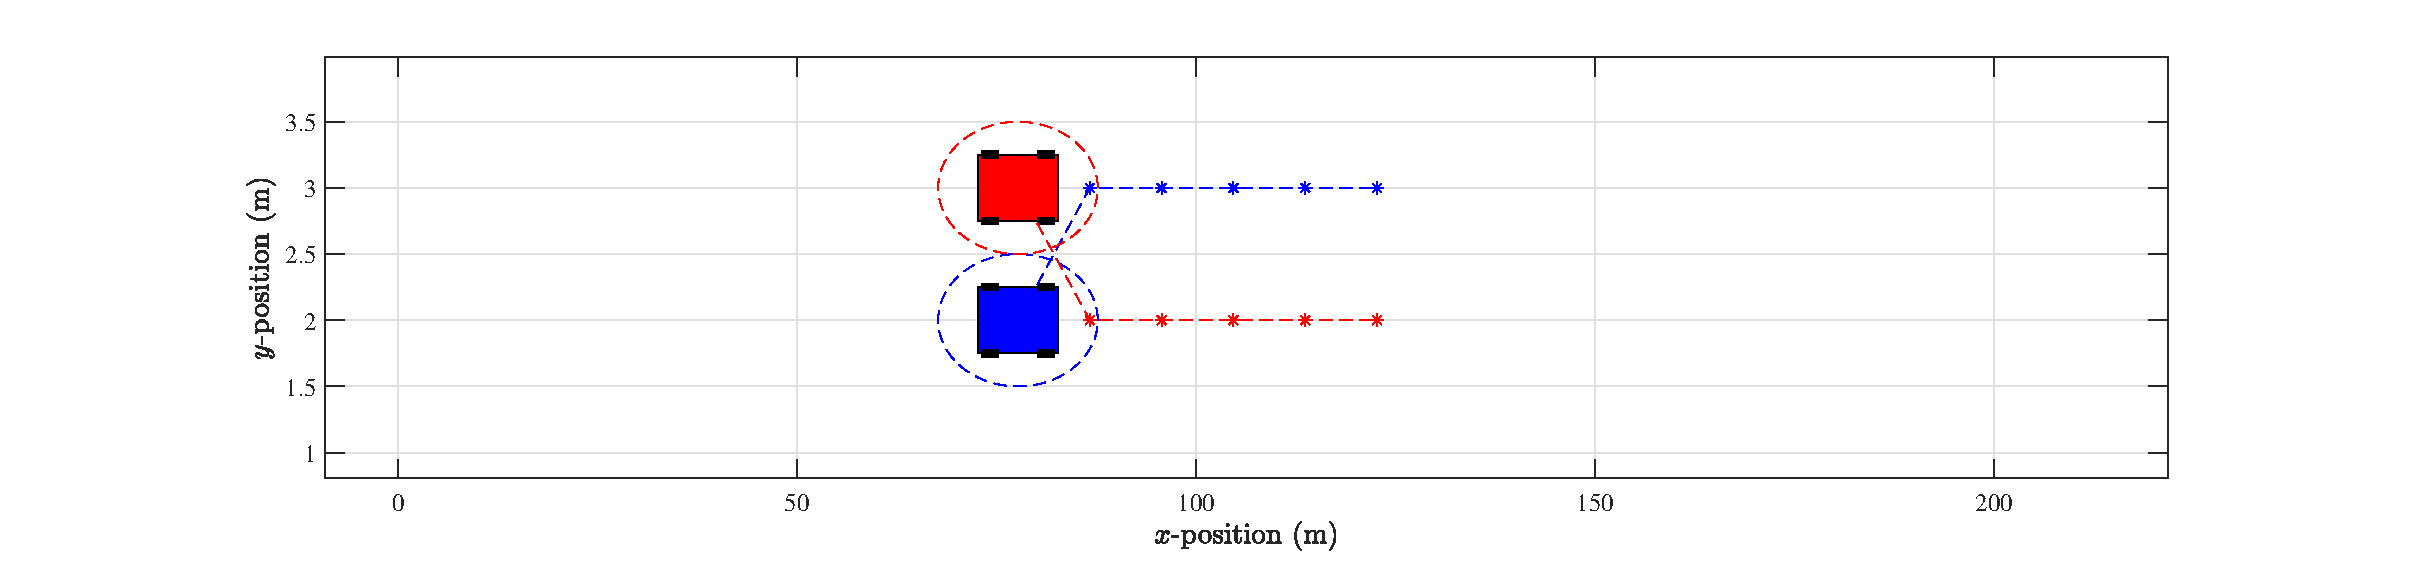
\includegraphics[width=0.95\textwidth]{Kap3/untitled.eps}
    \label{fig:lat_col1}
    \caption{Position of vehicles during the example.}
\end{subfigure}%
\vspace{1cm}
\begin{subfigure}[b]{1\textwidth}
\centering
    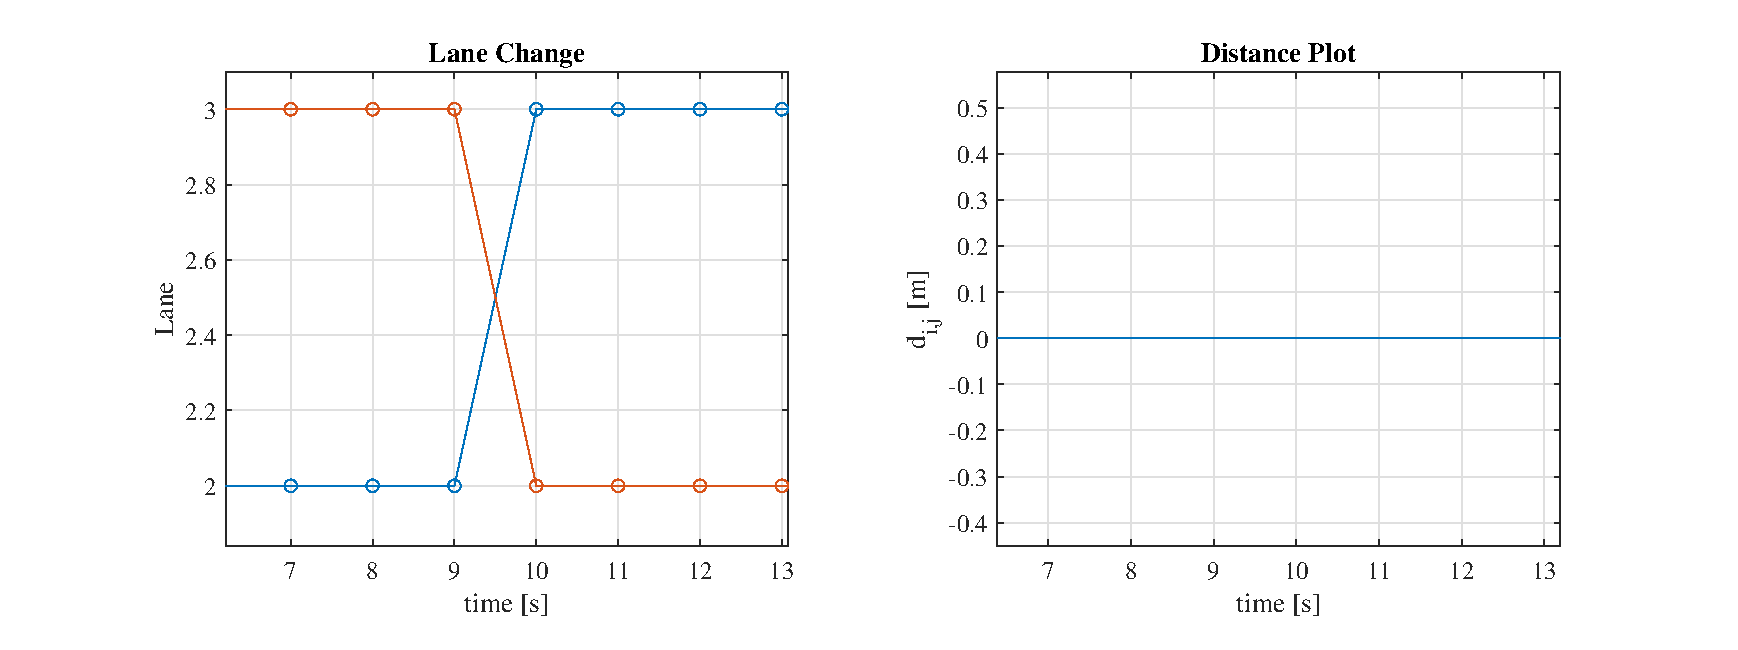
\includegraphics[width=0.95\textwidth]{Kap3/plot_change_line.eps}
    \caption{ Profiles of velocity and lanes over highway.}
    \label{fig:lat_col2}
\end{subfigure}
% \hfill
\caption{  Example of lateral collision.  }
\label{fig:lat_col}
\end{figure}

There are other common collisions in a regular lane; those are lateral collisions, usually generated by occlusion problems. This model does not have this issue thanks to interconnected and full neighbour position knowledge. However, the controller solver could be in a position where each vehicle decides to change at the same time the lane as Fig \ref{fig:lat_col} shows. Owing to this, we implement the lateral rule for each vehicle $i,j$ driving over the horizon $\mathcal{T}$, if the longitudinal distance $d_{i,j}$ is less than a safe distance and the difference of lane position $z_{i,j}$ is one $\left| z_{i,j} (t) \right|=1$, and the pair of agents will change the lane $z_{i} (t+1) \neq z_{i} (t), z_{j} (t+1) \neq z_{j} (t)$, the controller must constraint the change of lane as is explained in the next algorithm.

\begin{algorithm}
\caption{Algorithm of lateral distance}\label{alg:lat_saf}
\begin{algorithmic}
% \FOR $i \in \mathcal{V}$
% \FOR \forall {$i \in \mathcal{V}$} 
\If{ $\left| z_{i,j} (t) \right|=1$ and ($z_{i} (t+1) \neq z_{i} (t)$ or $ z_{j} (t+1) \neq z_{j} (t)$)}
    \If{$d_{i,j}(t) > 0 $}
        \State $d_j(v_j(t)) -d_i(v_i(t)) > D_s$
    \ElsIf{ $d_{i,j}(t) < 0$} 
        \State $d_j(v_j(t)) -d_i(v_i(t)) < -D_s$
    \Else
        
        \State Continue normal driving
    \EndIf
\EndIf

\end{algorithmic}
\end{algorithm}

Finally,  the previous safety rules are executed in a mixed-integer decision-making framework explained in-depth way in chapter \ref{nonlinear_model}. Nevertheless, this thesis work does not focus on the issue of communication among vehicles. Consequently, we assume that:
\begin{itemize}
\item Vehicles can share data of their position, speed, current lane and future states planned. 
\item Each vehicle is autonomous, therefore it has the capability to change its position and velocity without the presence or intervention of a human being
\end{itemize}








% \section{Robot Architecture}
% //////////////////////////////////////////////////////

% ##############################################


\subsection{Non-Linear Model System}
\label{nonlinear_model}
Currently, there are several kinds of wheel robots used for mobile applications. Some of them are unicycle, Ackerman, differential, and omnidirectional, among others. In \cite{81t} was compared the two main ways to represent a dynamic system and the kinetic and kinematic models were compared in the vehicle collision avoidance framework. Although the kinetic model has more accuracy than the kinematic, the entire system implemented in an MPC is faster with the kinematic model than with the kinetic model. Due to better prediction accuracy and computational time in the established prediction horizon, we decided to use the robot's kinematic model. 
\\
The nonlinear kinematic unicycle model is one of the most popular models for automated driving in multiagent systems \cite{kinematic} and mobile robotics. Therefore, we designed, fine-tuned, manufactured and implemented a linear unicycle model for the medium level of control. It makes the following assumptions:


\begin{itemize}
    \item Into the prediction horizon of the MPC., the velocity V could change.
    \item Forces are applied only in the lateral wheels, neither in the caster wheels.
    \item The robot is not equipped with a steering wheel.
    \item Aerodynamic drag and rolling resistance are ignored.
    \item The position of the front and rear caster wheel does not matter.
    \item The Center of Gravity (CG) position is assumed in the middle of the lateral wheels; the height is assumed to be zero since the vehicle's motion is planar.
    \item Pitch and roll dynamics are neglected. 
    \item The electrical energy and forces applied to the traction wheels are neglected.
\end{itemize}
\\

In order to specify the actual position of the robot within two-dimensional space, we use a relationship between the robot's global reference and the robot's local reference, as shown in Fig \ref{kinematic2}. The Axis X and Y define the position related to an origin $O: \left\{ X, Y \right\}$. The robot position is specified by three coordinates, $x, y$, and $\theta$, where $\theta$ is the angular position of the robot referred to as the global reference. It is also possible to describe the robot position as a vector of dimension three \ref{eq:vec_pos}.


\begin{equation}
\label{eq:vec_pos}
P_i= \begin{bmatrix}
x \\ 
y \\ 
\theta
\end{bmatrix}
\end{equation}

\subsubsection{Kinematic model of a differential robot}
Kinematics is one of the mechanic's branches that describes a particle's behaviour in an environment by the action of multiple forces regardless of its mass. Kinematic equations are used to express the motion of a point after the act of a force. The inputs interacting with the robot are the linear velocity $V [cm/s]$ and the angular velocity $w [rad/s]$. The rate of change of position of the vehicle in the x-direction and the y-direction are $x$ and $y$, respectively and are given by:

% the non-linear kinematic model of an unicycle robot could be represented in equation \ref{eq:nonlinear_model}.   
    
% {\color{blue}  buscar la manera de conectar el anterior parrafo con las ecuaciones del modelo y ademas agregar lo del introduction to autonomous mobile robotics,  de la pagina 73pdf}


\begin{equation}
\begin{split}
\label{eq:nonlinear_model}
\dot{x} =& v \cos{\theta}\\ 
\dot{y} =& v \sin{\theta} \\
\dot{\theta} =& \omega  \\ 
\end{split}
\end{equation}

Let $x_i, y_i$ be the lateral and longitudinal position of agent $i$ in the working space, and $\theta_i$ be the agent orientation. The $v_i$ is the linear velocity, and $w_i$ is the angular velocity. the control inputs variables are $v$ and $w$ and the output variables are the global position of the robot $x_i, y_i$ and $\theta_i$. Fig \ref{kinematic2} shows the representation of the mentioned variables.\

% {\color{blue} colocar un parrafo que hable de la cinematica interna del robot, que explique las variables de fierza de cada una de las rueaas, tambien que hable un poco de las leyes que rifen al robot por dentro guiarse del paper Motion planning and control }

\begin{figure}[h!]
\centering
    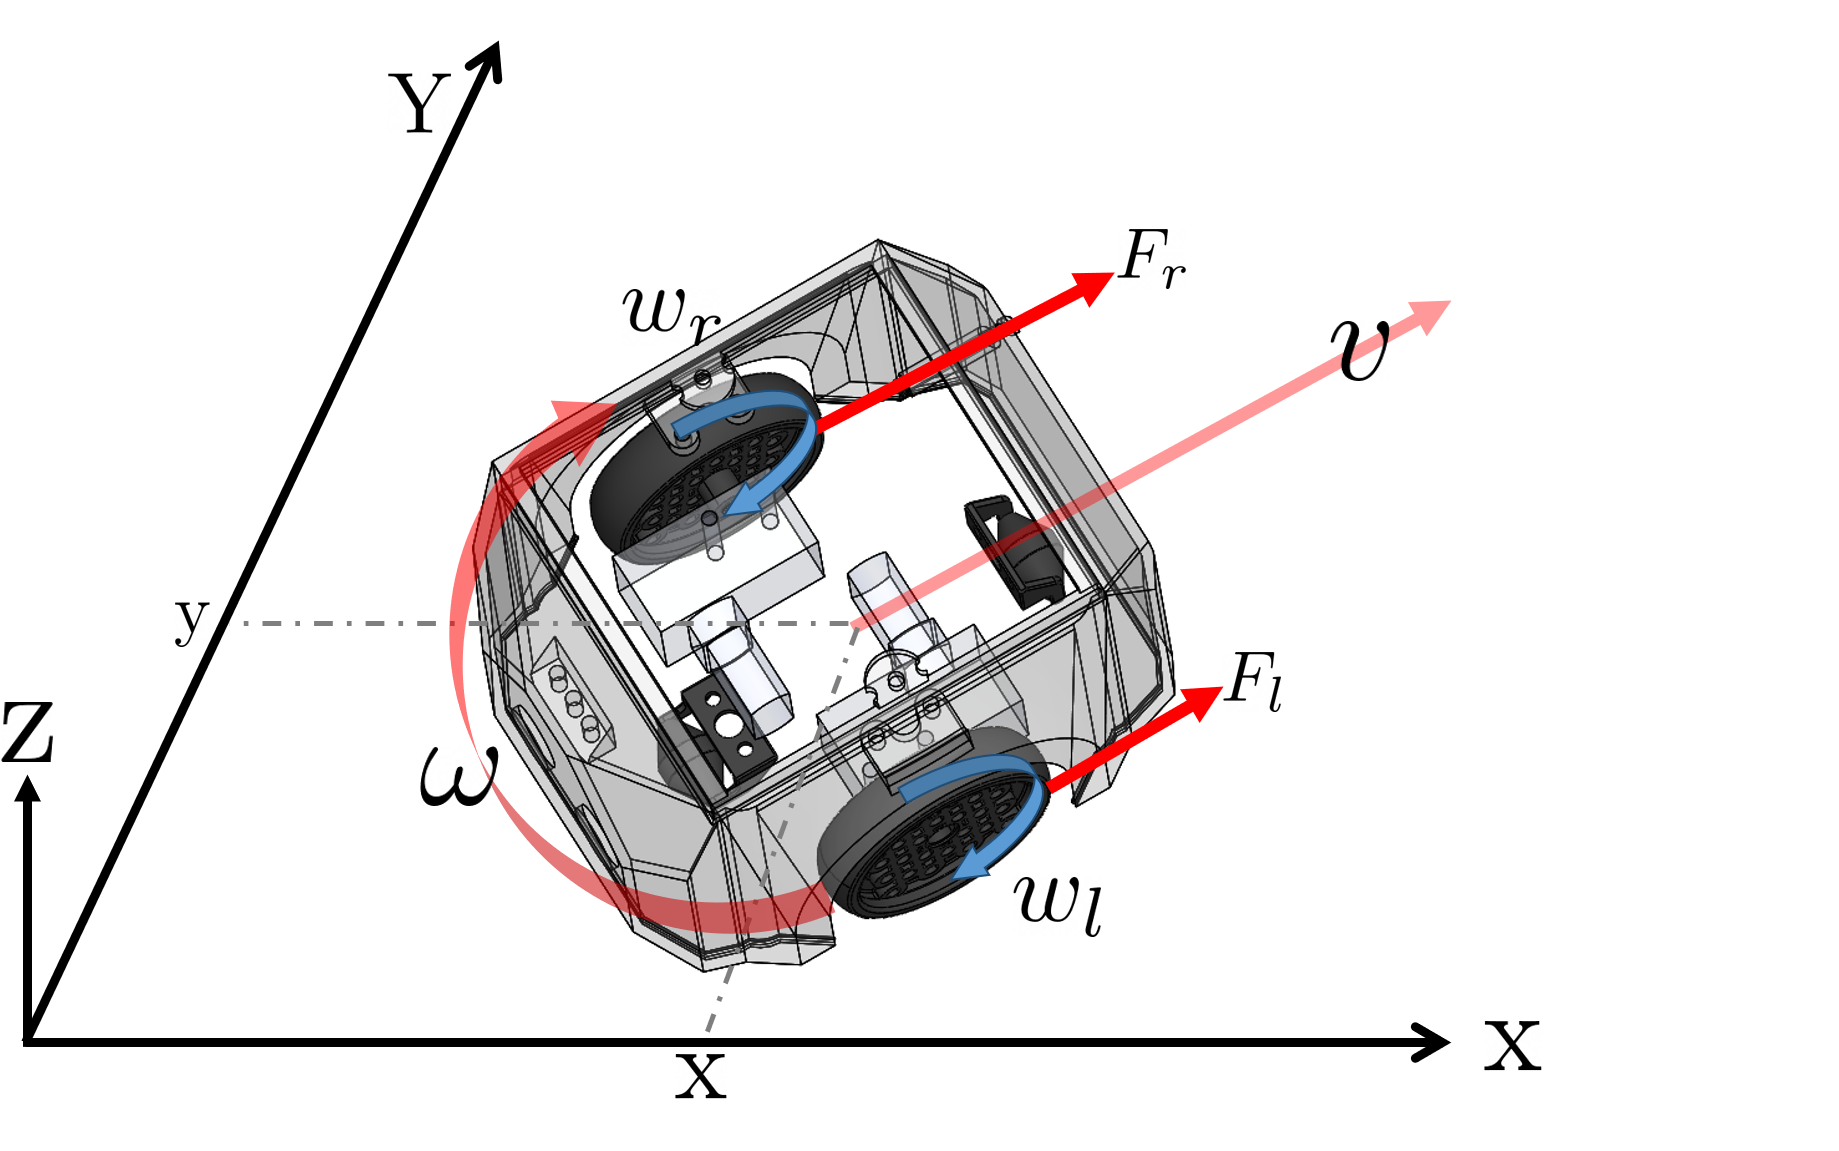
\includegraphics[width=0.8\textwidth]{Kap3/kinematic.png}
    \caption{Non-linear model of a differential robot.}
    \label{kinematic2}
\end{figure}




% ///////////////////////////////////////////////////////////////////




\subsection{Robot Model}
\label{robot_model}
% \begin{figure}[H]
% \centering
%     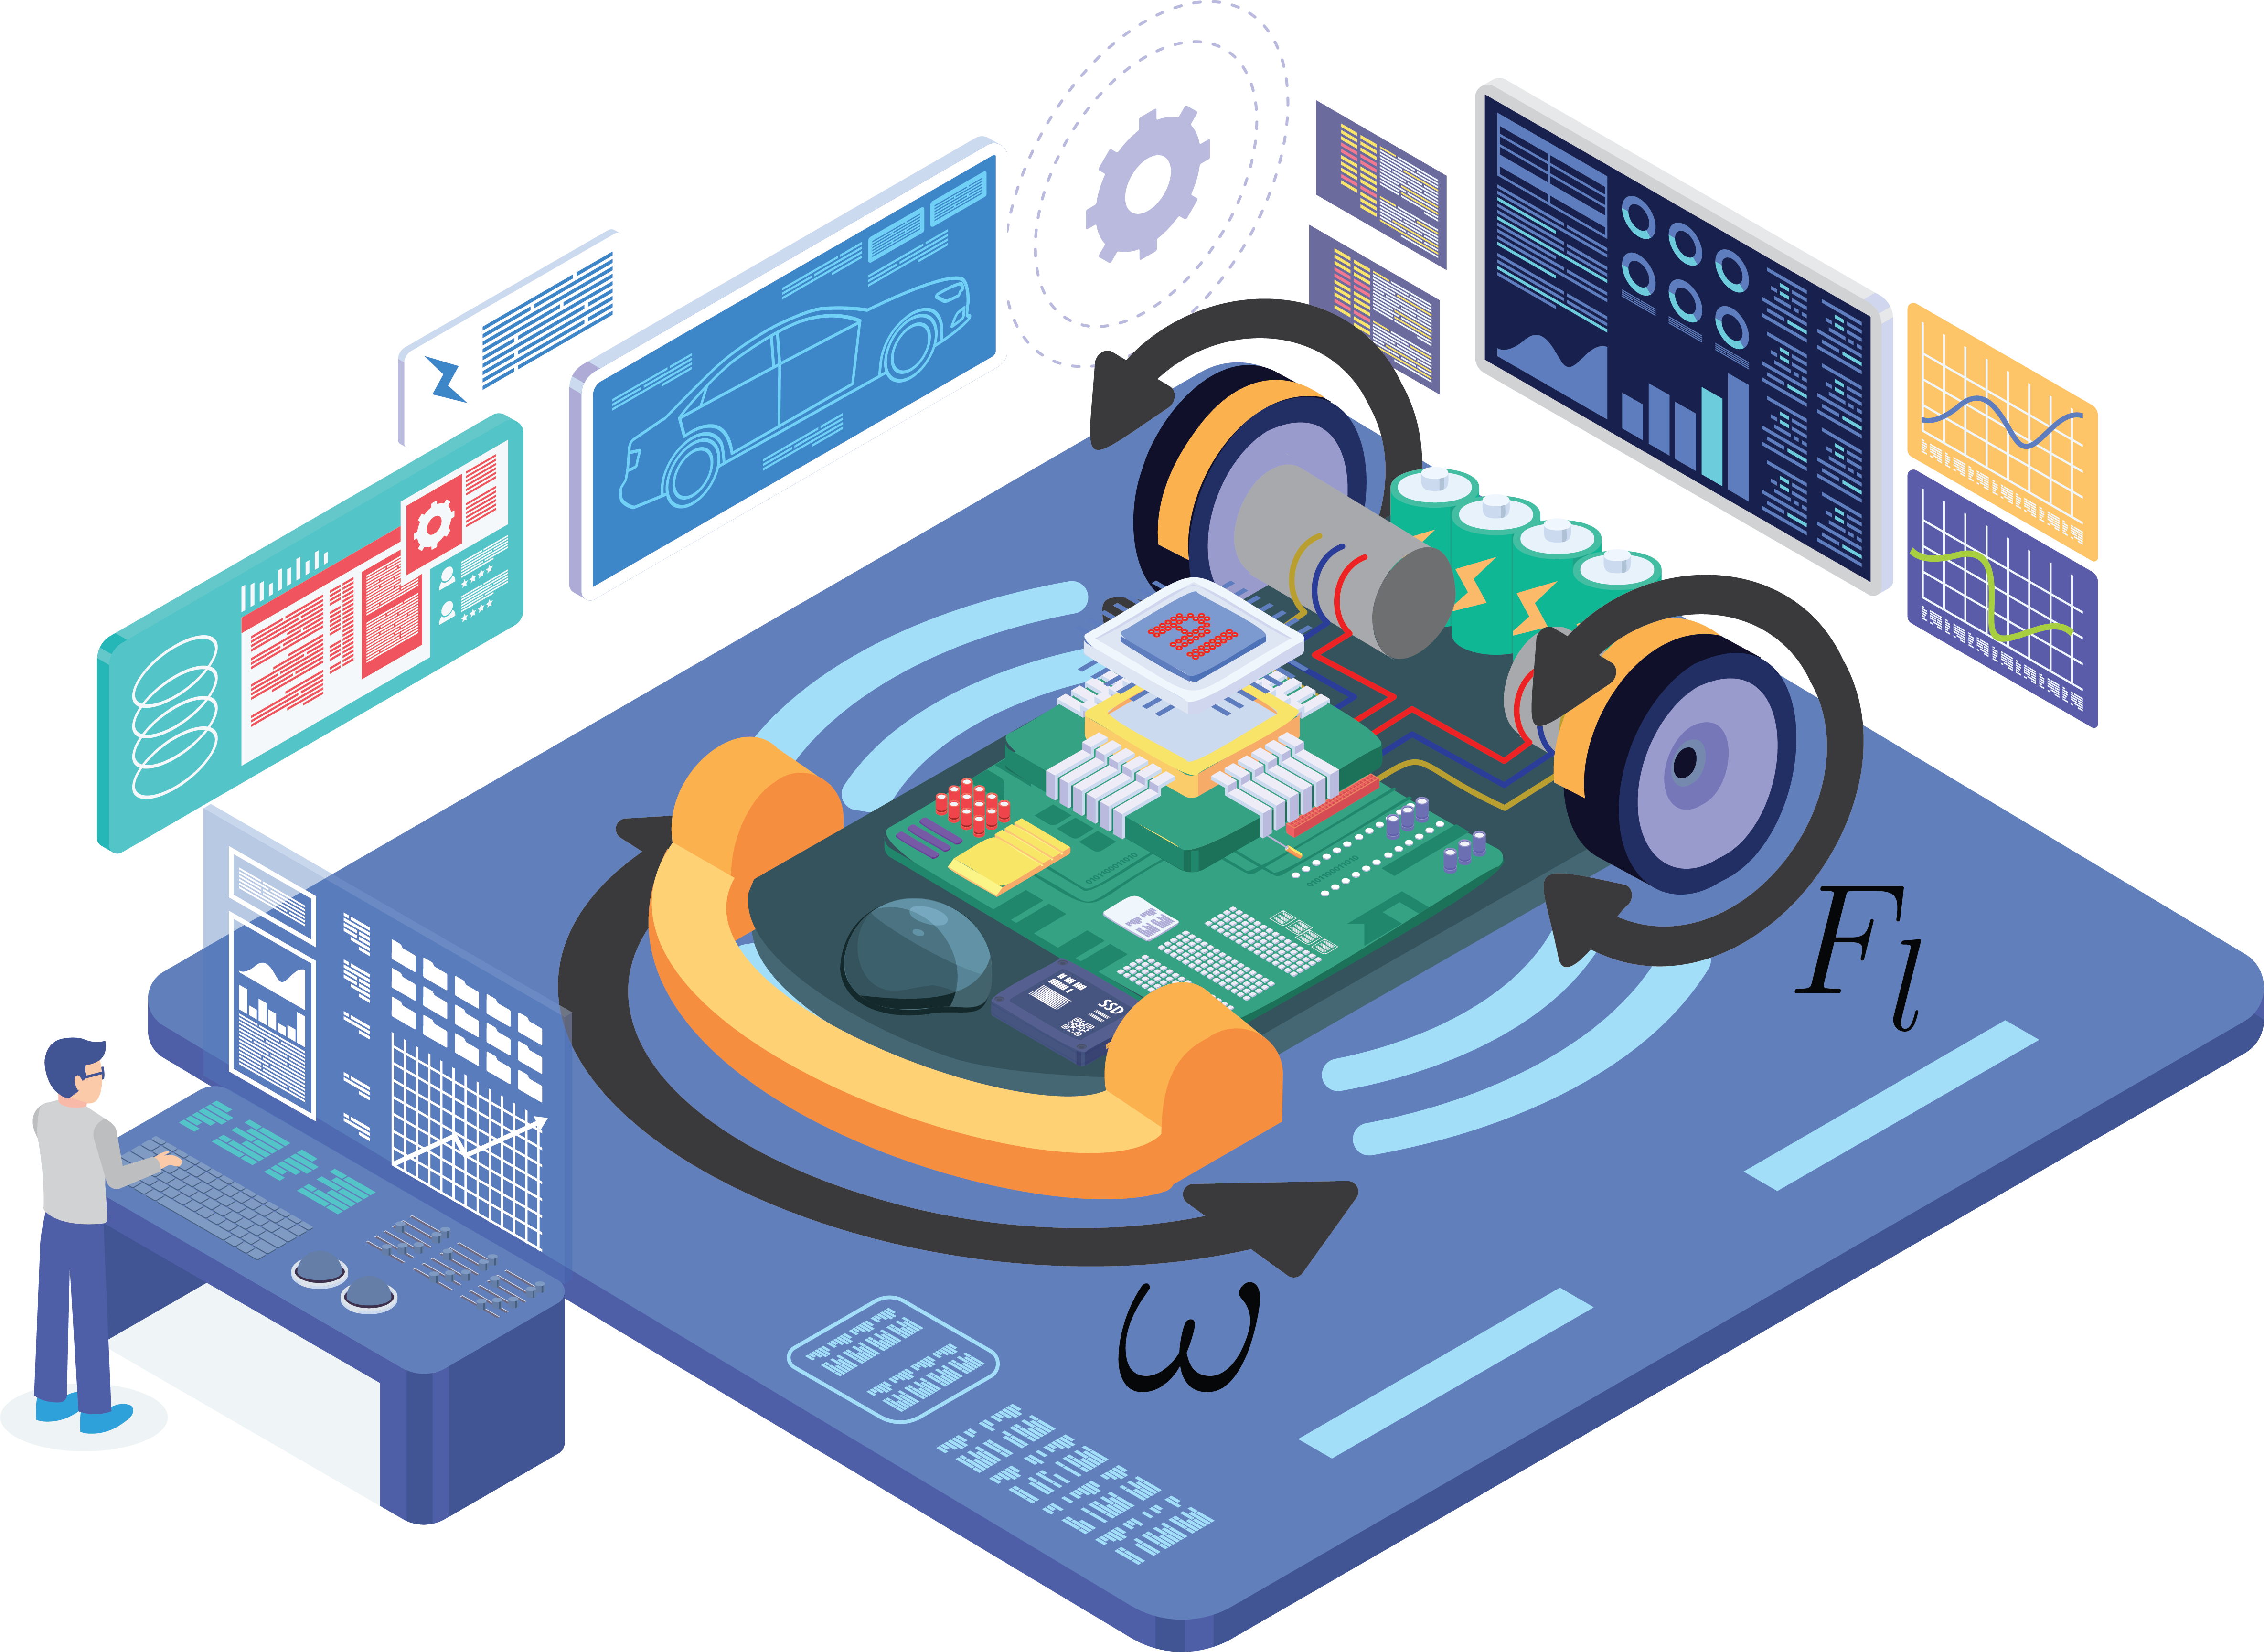
\includegraphics[width=0.4\textwidth]{Kap3/PID_model.png}
%     % \caption{Non-linear model of a differential robot.}
%     % \label{non_linearmodel}
% \end{figure}


% \subsubsection{Motion Control}




A unicycle model is unfeasible in the real world due to geometric constraints. However, it is good to model and control a particle object in an environment. Due to this, the robot uses a differential model in the low-level control architecture. This model allows calculating the control action in each wheel with only the information of linear and angular velocity. Equation \eqref{dif_equat} is the low-level model used to control each wheel's speed. Where $w_{r}$ and $w_{l}$ are the angular velocity of the right and left wheels, $L$ is the distance in cm between the two wheels, and $R$ is the radius of both wheels.

\begin{equation}
\begin{bmatrix}
\omega_{r}\\ \omega_{l}
\end{bmatrix} =  \frac{1}{2R}\begin{bmatrix}
2 & -L\\ 
2 & L
\end{bmatrix} \begin{bmatrix}
v\\ w
\end{bmatrix}.
\label{dif_equat}
\end{equation}


In pursuit of faster computation time and easy processing, we use the above model for the internal processing of the robot. The differential model is one of the most popular models used to simulate autonomous vehicles used in robotics. It was selected for its simplicity and the best results obtained. 
The actual robot uses this model to predict the position of the robot. The microprocessor calculates the speed required for each wheel to take the robot to a specific position. 

% {\color{red}  The main of this model is to get information about the wheels, motors, local environment, and the environment variables. The low-level control law can achieve the desired goal with the previous information. }


% {\color{red} Esta muy floja esta parte, siga escribiendo basese de buenas referencias, por ejemplo el capítulo 13 de (Planning algorithms- Steven M. LaValle) particularmente 13.1.2 Kinematics for Wheeled Systems }



% //////////////////////////////////////////////////////////////////////////////////////////////////
\section{Platform Design}

A test system was designed, built, and implemented to test the control algorithms used in this document in a real environment. The \ref{robot_model} section explains the model that the test robot uses in its control algorithm to find an optimal solution. This section will explain how the complete system is built and how it works. The \cite{agrobots} document explains this test system in deep.
All the test simulations shown in chapter \ref{chap:simulations} are implemented in this Testbed and are evidenced in the Annex \ref{AnexoA}.


\subsection{Robot Processing System}
\label{processing}
The Robot processing system was equipped with an Auriga board. This developing board contains an Atmega 2560 microcontroller running at 16 MHZ speed clock. In addition, the developing board has Gyroscope, thermistor, and a sound sensor for perception applications. Besides, it has a Bluetooth shield that allows microprocessor communication and programming, but it can be replaced for RF or WiFi modules. Moreover, it has 9 I2C ports, 1 UART port, and one port for ``smart motor'' applications.
The mainboard controls the encoder motors with a TB6612 chip. With the integration of this chip, the microprocessor can control with high precision the speed, direction and position of each wheel with an internal control closed loop.



%---------------------------------------------------------------------------

\subsection{Communication System}
The communication system considers the number of nodes and the bandwidth of the shared information. As a result, the ESP 8266 module was chosen due to its easy programming, powerful power processing, low-cost price and affordable. This communication system has a novel protocol to share information with the other agents without needing an external router. It can connect, transmit, and receive up to a 250-byte payload by WiFi network. This new protocol supports unencrypted peers. However, their total number should be less than 20, including encrypted peers. This protocol allows sharing information without requiring a WiFi station or router as a principal interconnection module. Besides, with this protocol, if one of the boards suddenly loses power or resets, it will automatically connect to its peer to continue the communication when it restarts. 

%---------------------------------------------------------------------------
\subsection{Global Position System}
\label{GPS}
The robot swarm are equipped with a fiducial marker system for camera pose estimation \cite{aruco}. This system uses a web camera and system image processing to detect and estimate the position of each robot. It is currently implemented using the OpenCV library in python language. The system can calculate $x,y,z$, and $\theta$ position of each agent. The platform uses as a visual sensor the Logitech C930 at a resolution of 1920x1080 pixels and a 90-degree field-of-view. It can achieve frame rates of up to 30 fps. This library can detect up to 1000 Aruco tags in the same frame.

%---------------------------------------------------------------------------
\subsection{Power System}
Each robot has a lithium-ion battery of 3000 mAh. It provides energy for about ten working hours. Moreover, the charging system recharges the battery in about 2 hours. This battery can provide up to 3 amps in a barrel and USB ports. The previous advantages make the power system robust and valuable to implement with different development boards. 


% //////////////////////////////////////////////////////////////
\subsection{The Interconnect System}

The Testbed was built by gathering multiple communication, tracking, processing, and sensing systems. All of them can be replaced in the future with better technologies or another system with better results.
\\

The process of operation of the Testbed is the following. The tracking system uses the OpenCV library and Aruco tags. The camera takes multiple frames to process the information, estimating the positions $x$, $y$, and orientation $\theta$. It gives a vector $p \in \mathbb{R}^{2,nr}$, where $n_{r}$ is the number of robots in each experiment.
\\

With this information, the central processing unit computes the value of the robot's control variables using the preferred technique. Then it broadcasts this information to each mobile robot via WiFi protocol. If the test needs feedback information, it will wait for it. Eventually, each robot gets data from the server, processes it, and makes a decision. 

The server can record, graph, and save all the information taken in each test. Additionally, it could record videos and process the previous information to analyze the data accurately. Figure \ref{diagram} is shown the connection of the entire Testbed and how each section interacts.

\begin{figure}[!h]
\begin{center}
    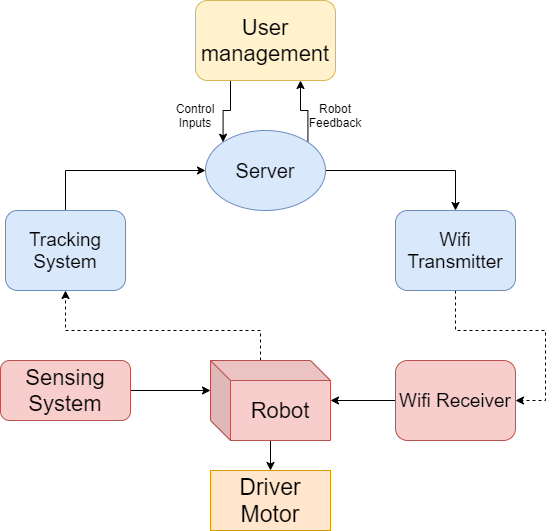
\includegraphics[width=13 cm]{Kap3/TestbedDiagram.png}
    \caption{System Architecture}
    \label{diagram}
\end{center}
\end{figure}


% {\color{Blue} agregar algun parrafo extra y mejorar la organizacion de esta seccion. }





\chapter{Controller Architecture}
% {\color{red} Excelente organización ahora a rellenarlo}
\section{Hight Level Control}

\subsection{D-ADMM}





\section{Mid Level Control}
\subsection{MIPG controller}

\subsubsection{Centralize MPC}

\subsubsection{Decentralized MPC}

\subsubsection{Cooperative MPC}

\subsubsection{Cooperative MPC}

\subsubsection{Potential Game}


\section{Low level control}

\subsection{DeePC}





\chapter{Simulation Results}


\chapter{Simulation}
\label{chap:simulations}

This chapter presents the results obtained in simulation for the MPC problem of path planning according to the parameters and conditions mentioned in the chapter \ref{chap:controller_evaluation}. In an unrestricted scenario with no change in environmental conditions or road conditions.
\\
\\
For the simulation, the following assumptions are taken:
\begin{itemize}
    \item All vehicles have the same dimensions.
    \item All vehicles have the same dynamic model, and there is no difference between them.
    \item The highway environment has no curves or intersections.
    \item The target speed and the desired lane are adjusted according to the interest of each driver.
\end{itemize}

\\
\\
The figures shown below are from different times. The initial time step shows the desired location and trajectories when $t_0=0$. In the time step, it is possible to see the most difficult maneuver to perform for some of the network agents. Finally, it is possible to see that everyone achieves their goal at the end of the control solution.
\\
\\
Colored squares represent vehicles, and circles represent possible crash risk areas. Colored dotted lines represent the predicted trajectories according to the agent to which they correspond. A final plot will be shown with as much information as possible in order to interpret the movement that the vehicles would have in a real scenario.
\\
\\
The main simulations were carried out with N=12 vehicles. However, simulations were made to analyze computation time with N = {2, 10} vehicles. First, the three most essential times in the simulation are shown, and then the quality and feasibility of each of the controllers will be discussed. In decentralized and centralized controllers, the trajectories are similar because the intention is to have the same working conditions. After a centralized and decentralized controller simulation, it is presented an analytic analysis. The analysis is based on the computation time as a function of the number of vehicles, the time per iteration of each controller, the increment of the computation time as a function of the prediction horizon, and the total simulation time as a function of the number of vehicles connected to the net. At the end of each section, a conclusion of each scenario will be given.
\\
\\
The solution algorithm is solved in MATLAB \cite{Matlab}. OCPs are solved using the GUROBI mathematical optimization engine with the YALMIP programming interface. GUROBI optimization engine is chosen to solve most problems due to its powerful branch and bound algorithm. With this, it is possible to solve mixed-integer quadratic programming problems (MIQP) in the presence of non-linear models. This section of the document seeks to evaluate the behavior of vehicles in a selfish environment dealing with selfish agents and trying to reach their goal. 


\section{Unrestricted Scenario.}

The unrestricted scenario is designed with 12 vehicles on the same road. It also has six lanes in line, and the road is one-way. There are no intersections, traffic lights, obstacles, crossings, or any obstructions in the simulation environment.


\begin{figure}[h!]
\centering
\begin{subfigure}[t]{\textwidth}
    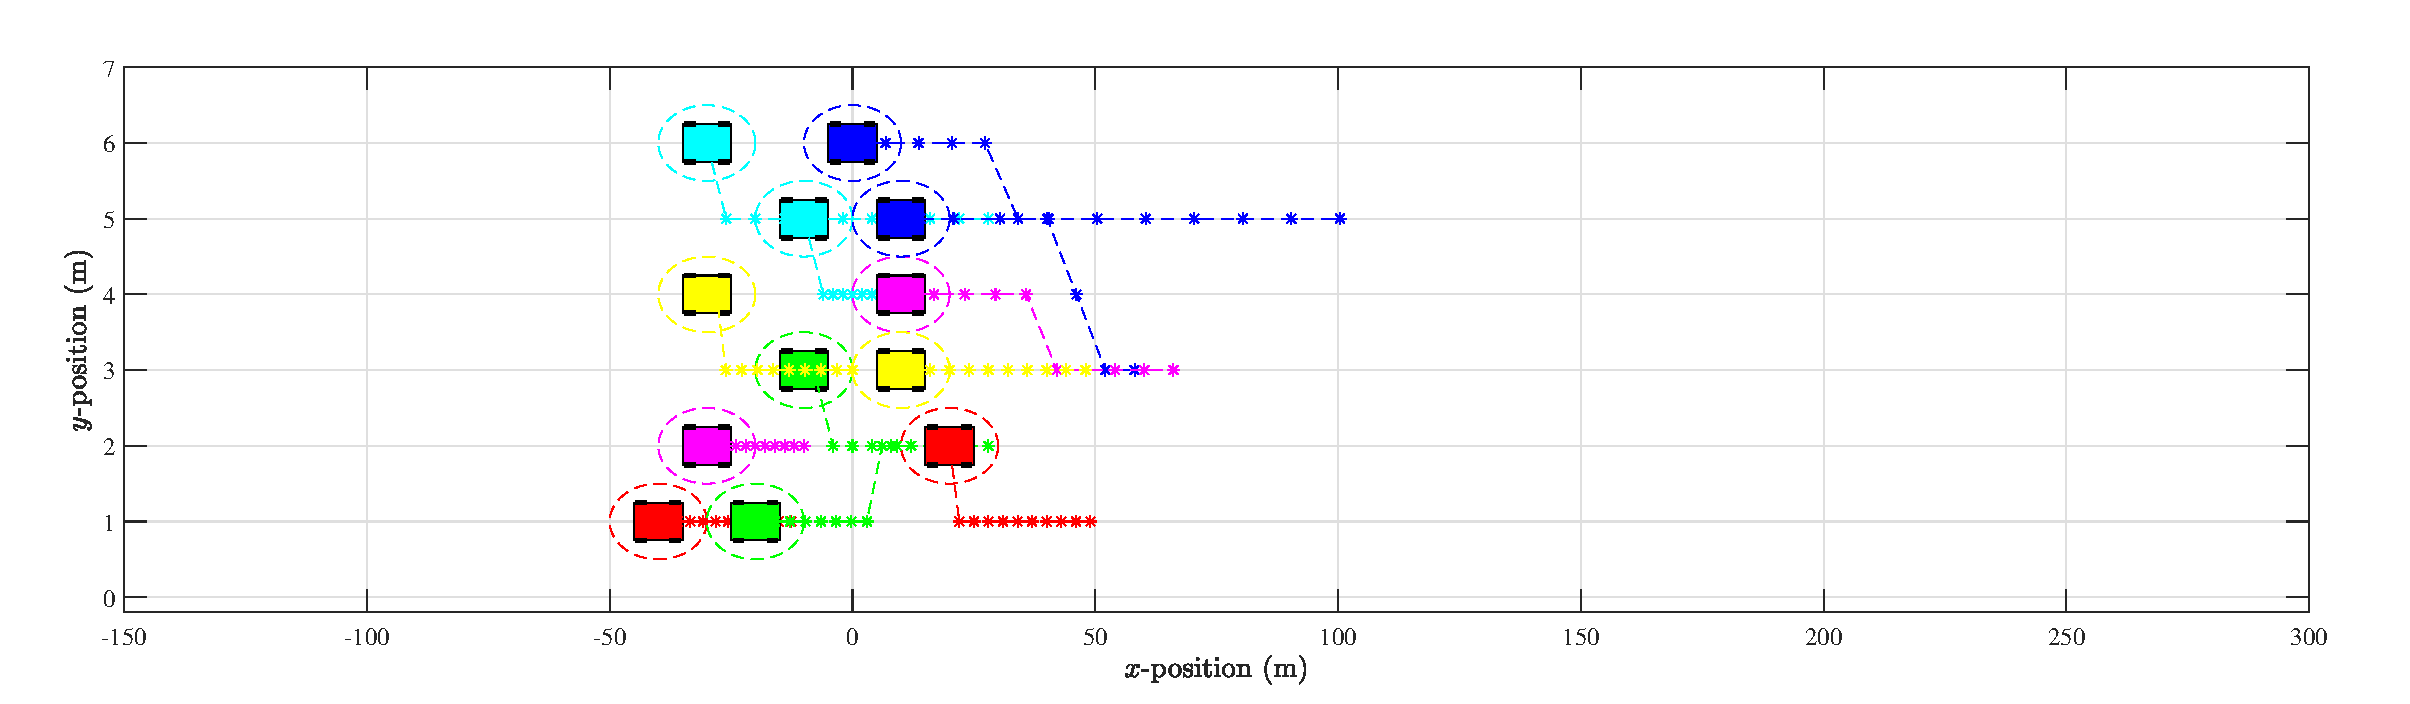
\includegraphics[width=\textwidth]{Kap6/no_restricted/no_restricted_traj0.eps}
    % \caption{Predicted positions.}
    \label{fig:first}
\end{subfigure}
\vspace{1cm}
\begin{subfigure}[b]{0.45\textwidth}
    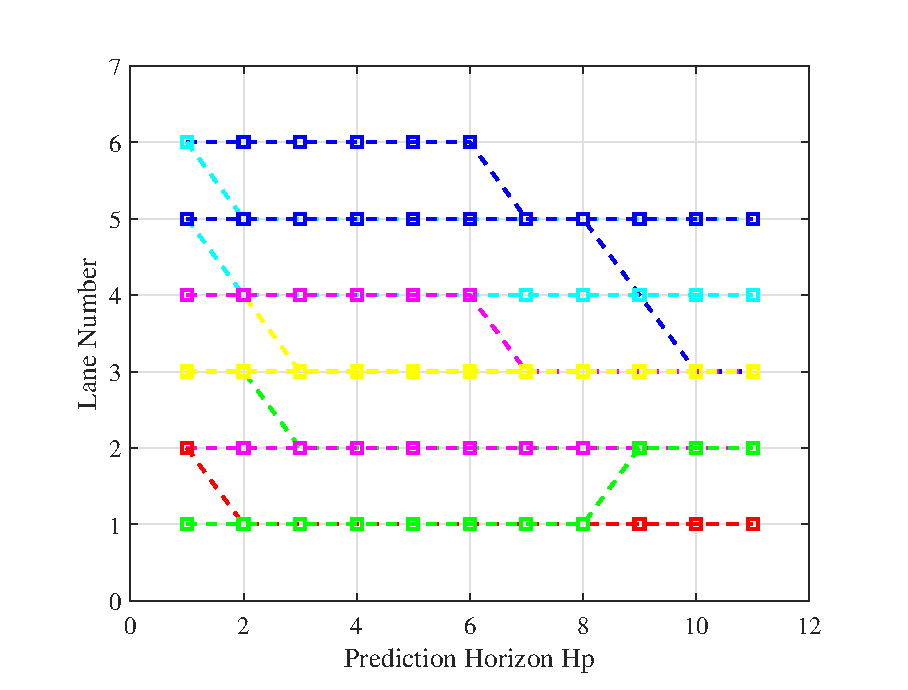
\includegraphics[width=\textwidth]{Kap6/no_restricted/no_restricted_lane0.eps}
    % \caption{Predicted lane profiles.}
    \label{fig:second}
\end{subfigure}
\hfill
\begin{subfigure}[b]{0.45\textwidth}
    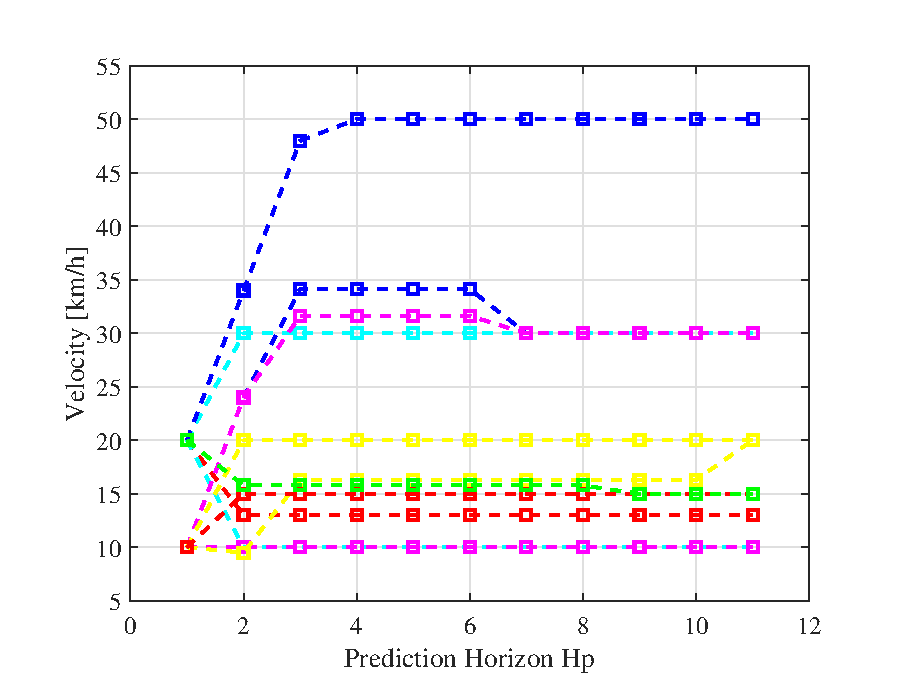
\includegraphics[width=\textwidth]{Kap6/no_restricted/no_restricted_vel0.eps}
    % \caption{Predicted velocity profiles.}
    \label{fig:third}
\end{subfigure}
\caption{MPC Iteration = 0. Initial conditions}
\label{fig:figures}
\end{figure}

\vspace{0.5cm}
At the beginning of the simulation, the vehicles are adjusted to an initial position and speed, as explained in more detail in the \ref{subsec:descentr} chapter. As seen in the image in the first step, each of the agents has a predicted trajectory taking into account the predicted trajectories of its neighbors.


% /////////////////////////////////////////////////
% ..........................................
\begin{figure}[h!]
\centering
\begin{subfigure}[t]{\textwidth}
    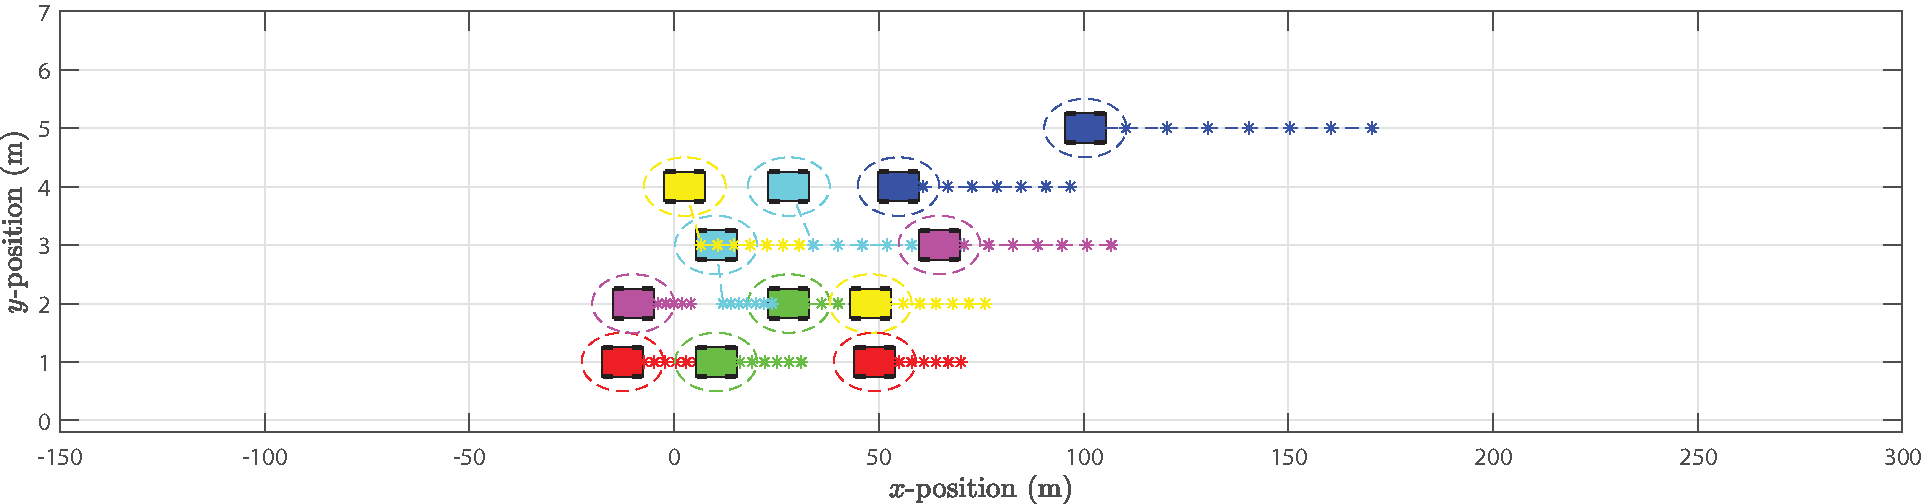
\includegraphics[width=\textwidth]{Kap6/no_restricted/no_restricted_traj10.eps}
    \caption{Predicted position.}
    \label{fig:first}
\end{subfigure}
\vspace{1cm}
\begin{subfigure}[b]{0.45\textwidth}
    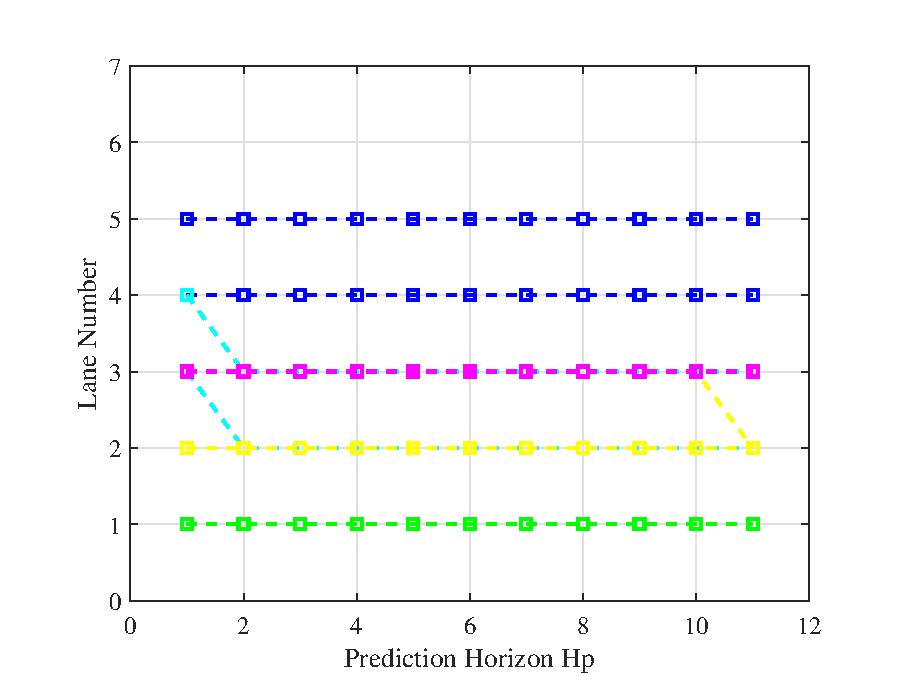
\includegraphics[width=\textwidth]{Kap6/no_restricted/no_restricted_lane10.eps}
    \caption{Predicted lane positions.}
    \label{fig:second}
\end{subfigure}
\hfill
\begin{subfigure}[b]{0.45\textwidth}
    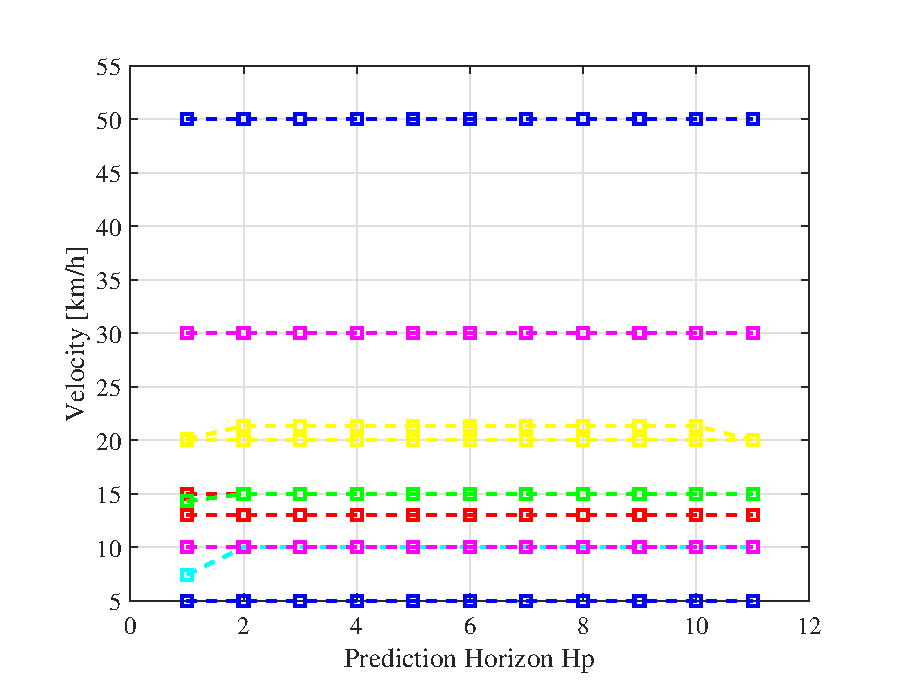
\includegraphics[width=\textwidth]{Kap6/no_restricted/no_restricted_vel10.eps}
    \caption{Predicted velocity profiles.}
    \label{fig:third}
\end{subfigure}
\caption{MPC Iteration = 10. Vh 2,3,4,6 change lanes.}
\label{fig:figures}
\end{figure}

In the first scenario, the centralized and decentralized controllers achieve the main objective of each of the agents. The trajectories travelled during the simulation time in both cases are the same because the initial conditions and the main objective are the same. Therefore, the paths shown are equivalent for both network architectures.

% .........................................
\begin{figure}[H]
\centering
\begin{subfigure}[t]{\textwidth}
    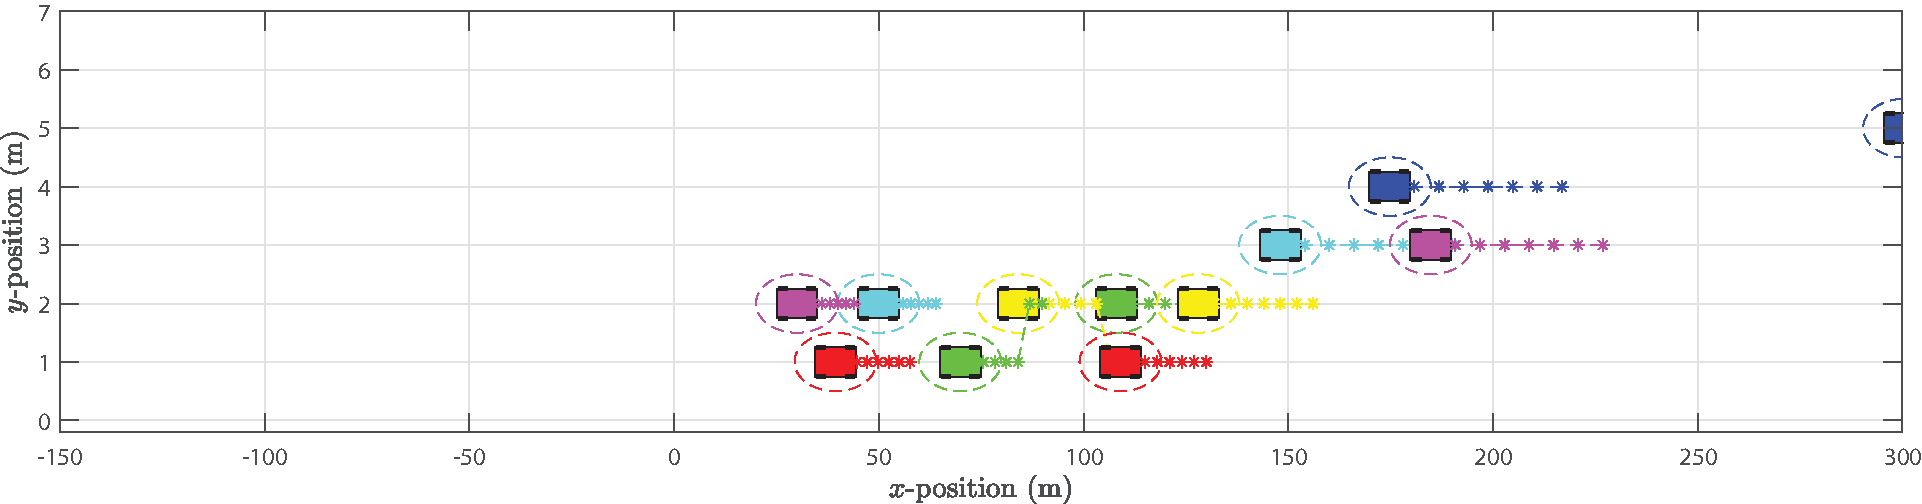
\includegraphics[width=\textwidth]{Kap6/no_restricted/no_restricted_traj30.eps}
    \caption{Predicted position at first position.}
    \label{fig:first}
\end{subfigure}
\vspace{1cm}
\begin{subfigure}[b]{0.45\textwidth}
    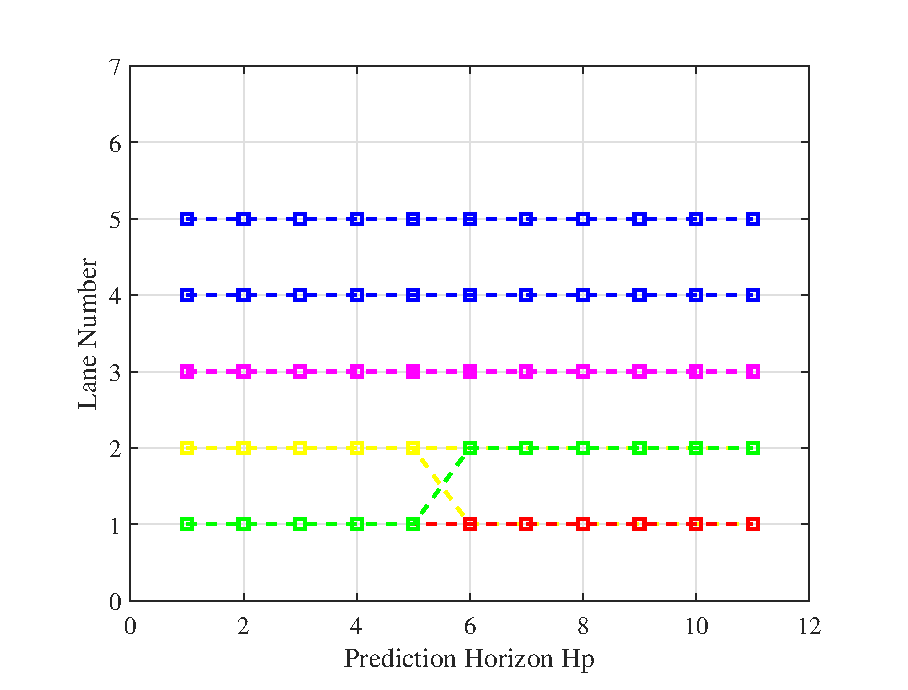
\includegraphics[width=\textwidth]{Kap6/no_restricted/no_restricted_lane30.eps}
    \caption{Predicted lane positions.}
    \label{fig:second}
\end{subfigure}
\hfill
\begin{subfigure}[b]{0.45\textwidth}
    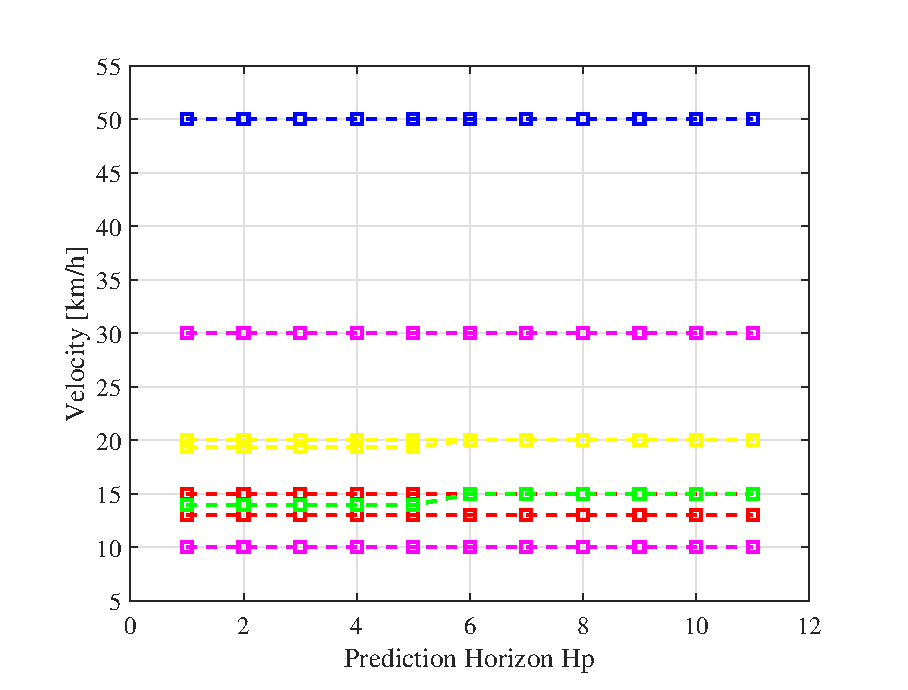
\includegraphics[width=\textwidth]{Kap6/no_restricted/no_restricted_vel30.eps}
    \caption{Predicted velocity profiles.}
    \label{fig:third}
\end{subfigure}
\caption{MPC Iteration = 30. The overall goal of the network is achieved }
\label{fig:figures}
\end{figure}
% .......................................

\\

\begin{figure}[H]
\centering
    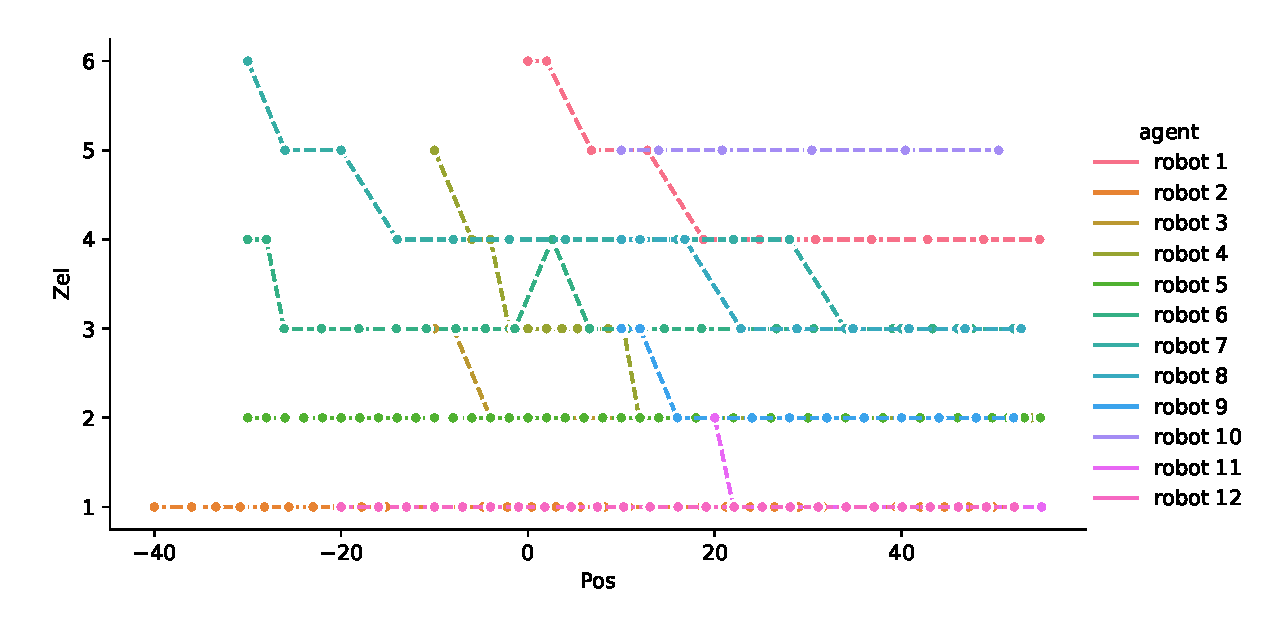
\includegraphics[width=0.8\textwidth]{Kap6/no_restricted/no_restricted_trajectories.eps}
    \caption{Trajectories of the entire network during the simulation time.}
\end{figure}

% ////////////////////////////



\\

% \subsection{Computation Time}
\vspace{0.5cm}
The computation time of D-MPC during the entire simulation is computed with the mean of each step sample. In Fig \ref{Step_time_no_rest}, it can see the average time that the network takes to solve each step $k$ of the solution algorithm. In addition, the time taken by the fastest controller (lower barrier) and the slower controller (upper barrier) is shown. The time it takes for each agent to resolve its OCP depends on the environmental conditions and the main objective it is looking for.
\\
\begin{figure}[H]
\centering
    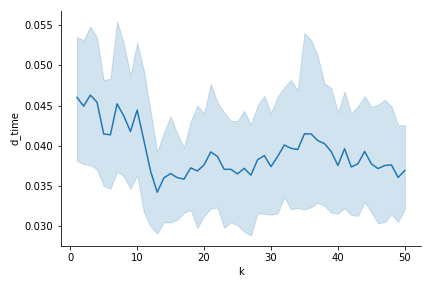
\includegraphics[width=.6\textwidth]{Kap6/no_restricted/no_restricted_d_time.png}
    \caption{Step time}
        \label{Step_time_no_rest}
\end{figure}

% ...........................



\begin{figure}[h!]
\centering
    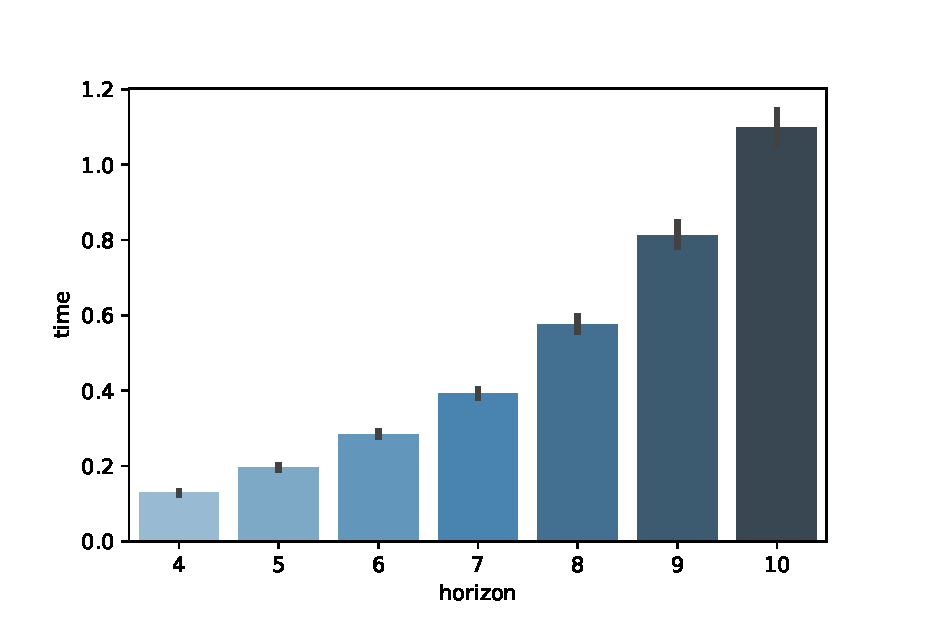
\includegraphics[width=0.6\textwidth]{Kap6/no_restricted/no_restricted_horizon_time.eps}
    \caption{Non-linear model of a differential robot.}
    % \label{kinematic2}
\end{figure}

Finally, an analysis of the time difference in the architectures is made. It is remarkable to see the improvement of the D-MPC networks. However, for real-time driving, the solution time is not enough.

\begin{figure}[H]
\centering
    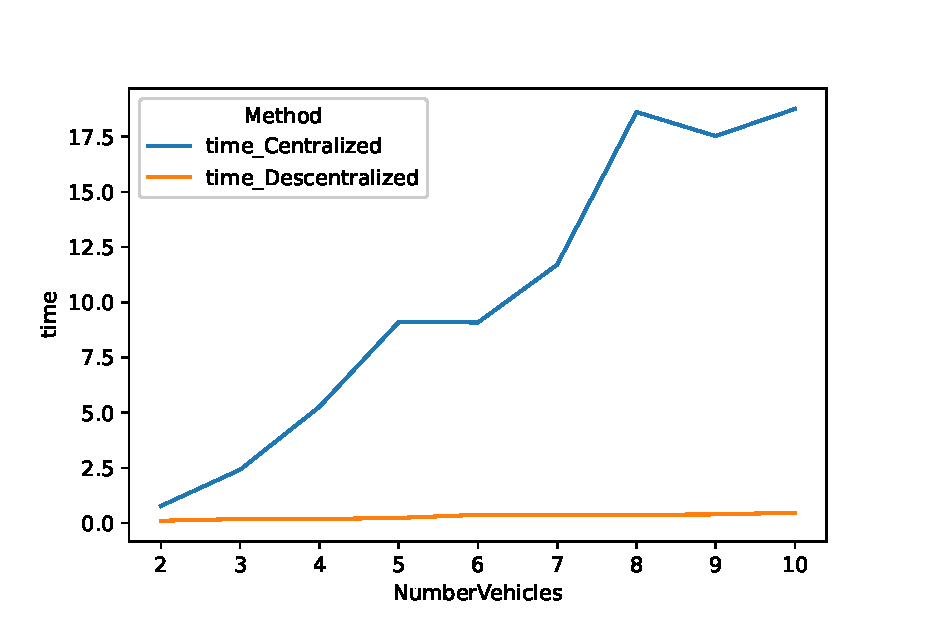
\includegraphics[width=0.6\textwidth]{Kap6/no_restricted/no_restricted_n_vehicles.eps}
    \caption{Computation time vs Number of vehicles.}
    % \label{kinematic2}
\end{figure}



% % ...........................
% \subsubsection{Trajectory Quality}

% ...........................
% \subsubsection{Controller Comparison - Unrestricted scenario}

% ...........................
\subsubsection{Conclusion Unrestricted Scenario}

Both control structures (C-MPC and D-MPC) show that autonomous driving is possible in a highway environment. The Potential game's framework allows the controller to take into account the conditions of others and make the optimal decisions in selfish scenarios.
\\
\\
Given the time results, it can be concluded that in a highway scenario, it is not possible to drive a vehicle with this technique due to the lack of computing power that we currently have to be able to solve this problem in a specific time. Solution times in D-MPC are much lower than what is seen in C-MPC. The C-MPC manages to give an optimal solution, but its solution takes a long time. Also, sometimes the controller falls into local minimums but fails to reach a global minimum.

\newpage
% -------------------------------------------
\section{Obstacle Avoidance Scenario}
% -------------------------------------------

The obstacle avoidance scenario was designed with 12 vehicles on the same road. It also has six lanes in line, and the road is one-way. There is one vehicle in the lane $L=3$  with no movement. It represents an obstacle that the controller's vision system could recognize. The main objective is to prevent the damaged vehicle from achieving its objective speed and lane.

\begin{figure}[H]
\centering
\begin{subfigure}[t]{\textwidth}
    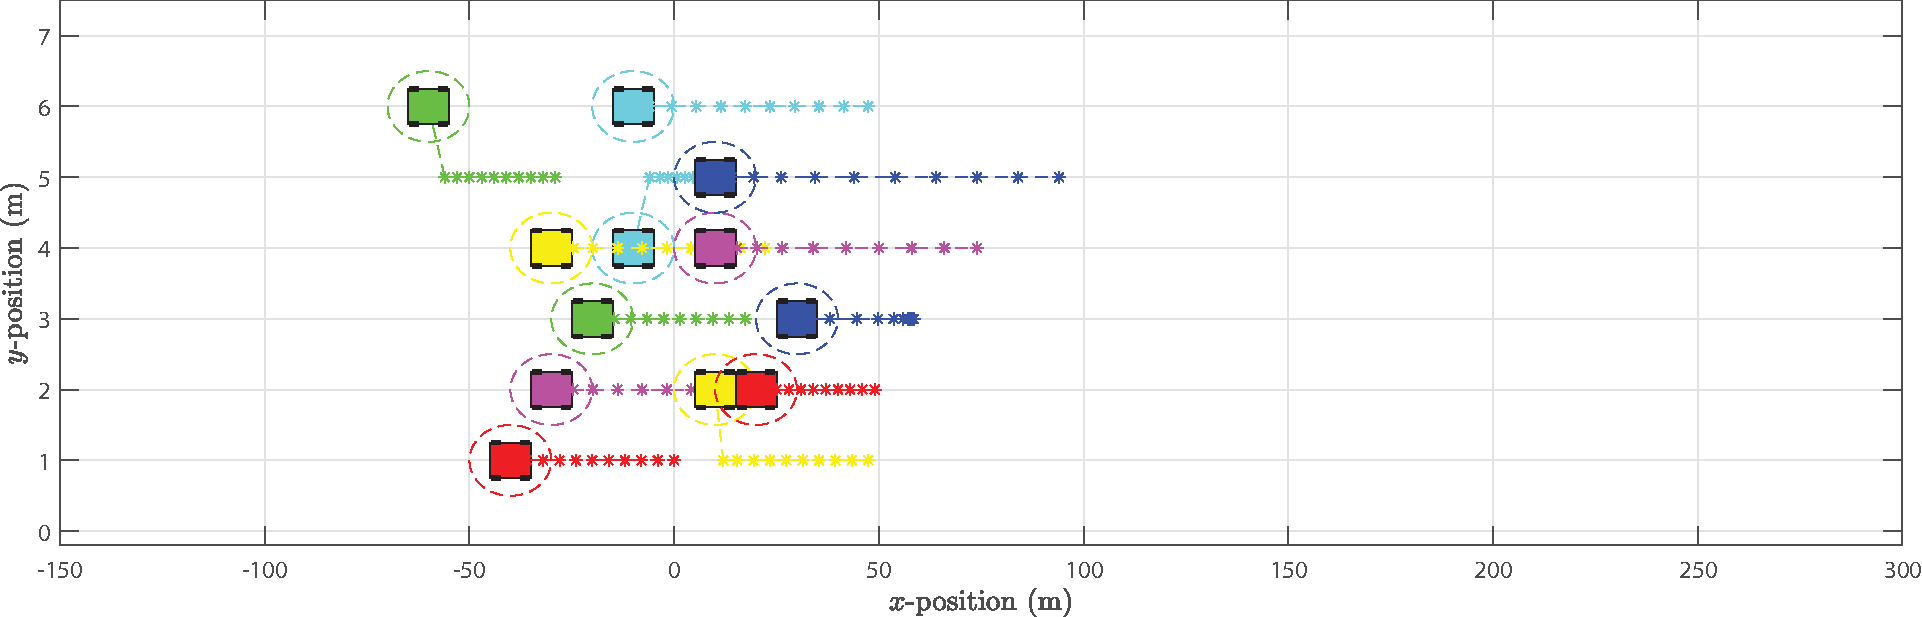
\includegraphics[width=\textwidth]{Kap6/obs_avoid/obs_avoid_traj0.eps}
    \caption{Predicted positions.}
    \label{fig:first}
\end{subfigure}
\vspace{1cm}
\begin{subfigure}[b]{0.45\textwidth}
    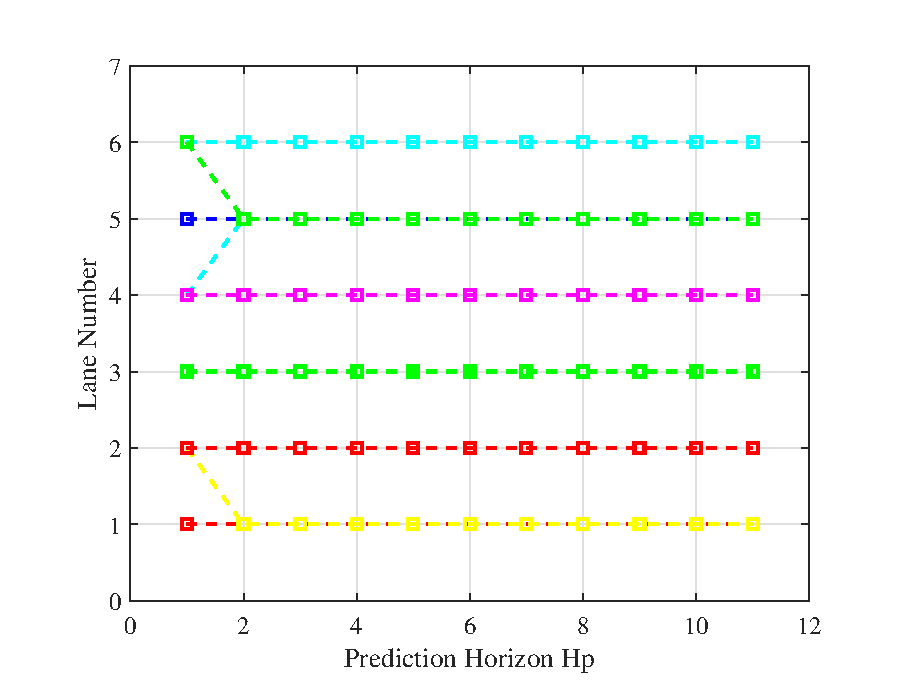
\includegraphics[width=\textwidth]{Kap6/obs_avoid/obs_avoid_lane0.eps}
    \caption{Predicted lane profiles.}
    \label{fig:second}
\end{subfigure}
\hfill
\begin{subfigure}[b]{0.45\textwidth}
    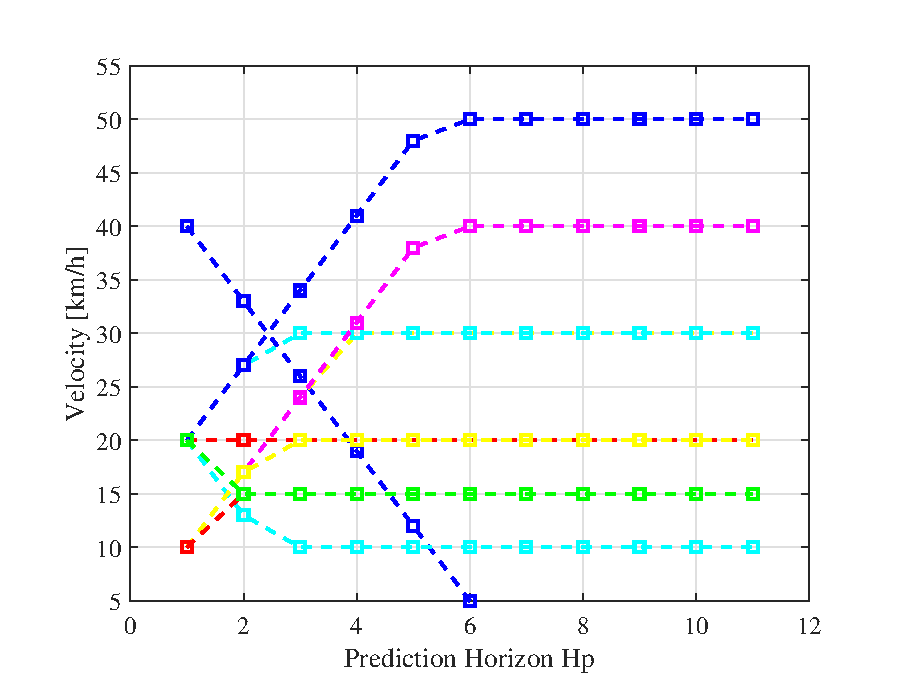
\includegraphics[width=\textwidth]{Kap6/obs_avoid/obs_avoid_vel0.eps}
    \caption{Predicted velocity profiles.}
    \label{fig:third}
\end{subfigure}
\caption{MPC Iteration = 0.}
\label{fig:figures}
\end{figure}

In iteration 0, the controller adjusts the initial positions of all the vehicles and the initial conditions. The scenario poses a vehicle blocked on the road so that the vehicle detection system can detect this new obstacle. It is essential to mention that in the first step, three vehicles are planning in their path plans to change lanes. Those are the only vehicles that can change lanes. In addition, the rest of the neighbors do not plan to change lanes because they have vehicles around them.
\\

% ........................................
\begin{figure}[H]
\centering
\begin{subfigure}[t]{\textwidth}
    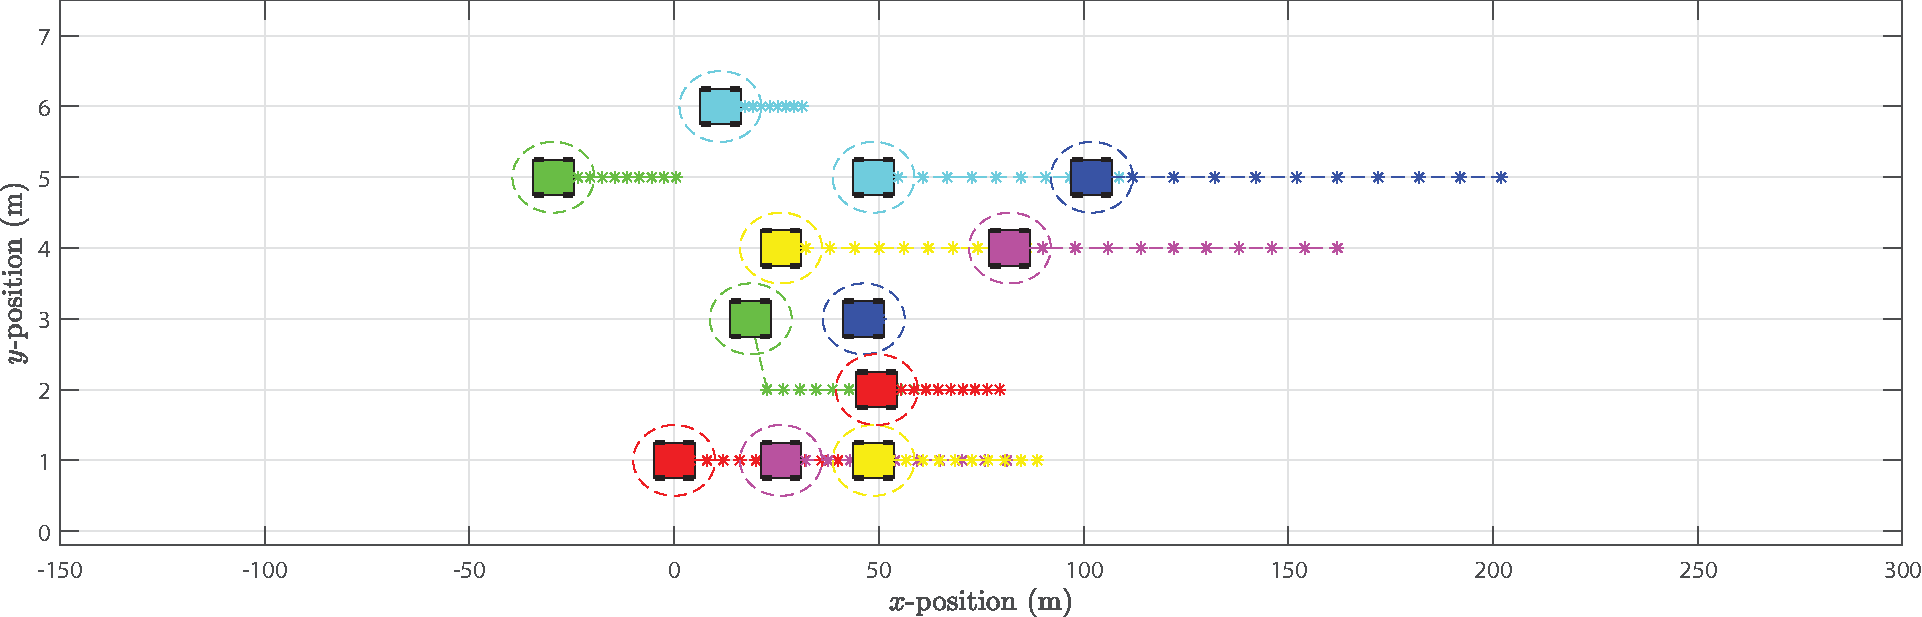
\includegraphics[width=\textwidth]{Kap6/obs_avoid/obs_avoid_traj20.eps}
    \caption{Predicted position.}
    \label{fig:first_mpc10}
\end{subfigure}
\vspace{1cm}
\begin{subfigure}[b]{0.45\textwidth}
    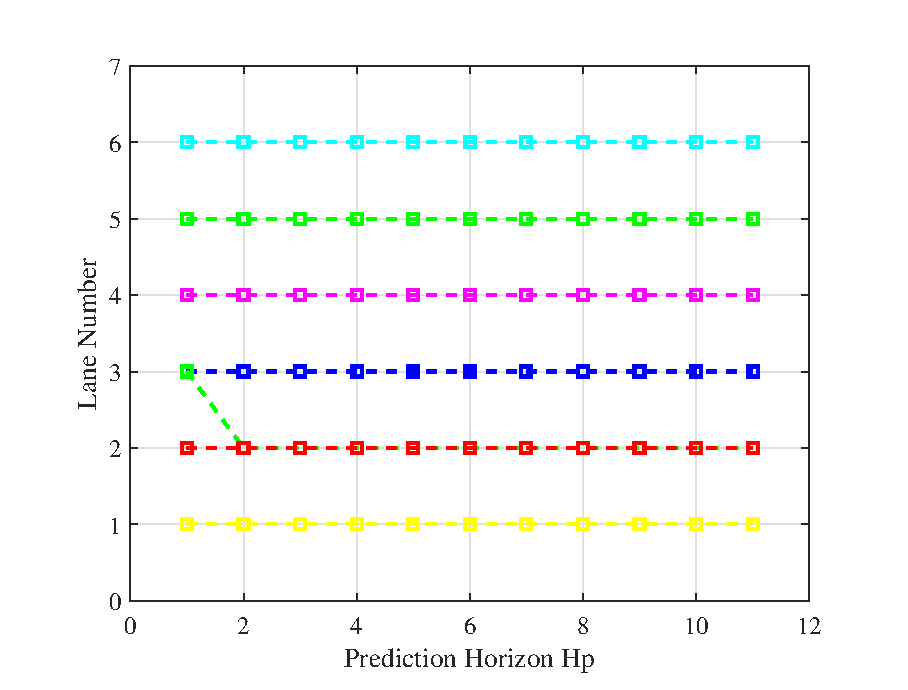
\includegraphics[width=\textwidth]{Kap6/obs_avoid/obs_avoid_lane20.eps}
    \caption{Predicted lane positions.}
    \label{fig:second_mpc10_obsav}
\end{subfigure}
\hfill
\begin{subfigure}[b]{0.45\textwidth}
    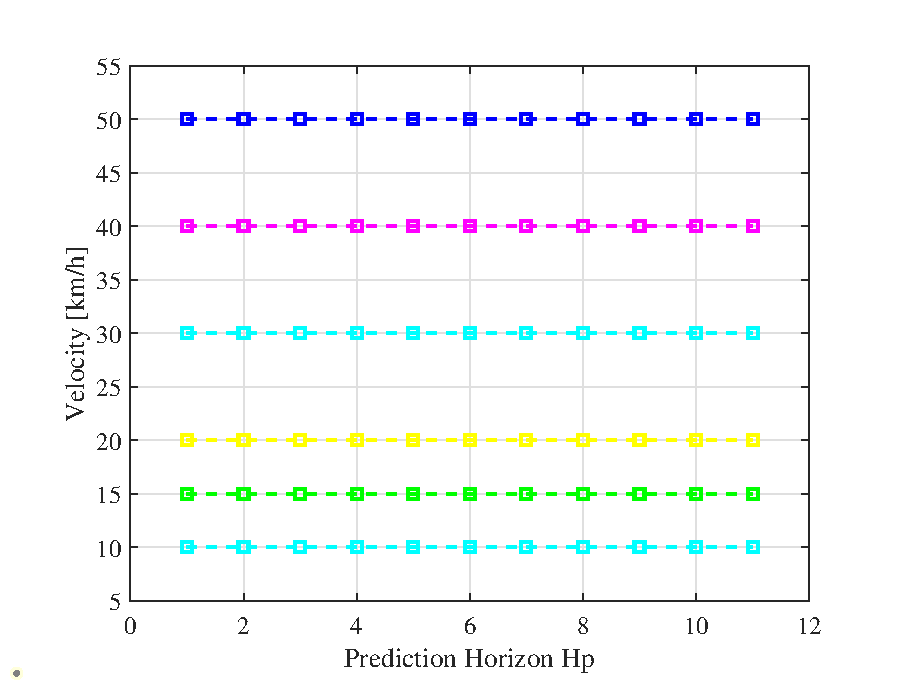
\includegraphics[width=\textwidth]{Kap6/obs_avoid/obs_avoid_vel20.eps}
    \caption{Predicted velocity profiles.}
    \label{fig:third}
\end{subfigure}
\label{fig:obs_mpc10}
\caption{MPC Iteration = 10.}
\end{figure}



In fig \ref{fig:first_mpc10}, it is possible to notice how vehicle number 3 (green color) has a trajectory prediction avoiding the obstacle. In addition, the other vehicles have changed lanes avoiding the obstacle. The vehicles $\mathcal{V}= \left\{ 4,2,5 \right\}$ (color red, purple, yellow) have already reached their desired lane without colliding with the others. In fig \ref{fig:second_mpc10_obsav}, the vehicles are not planning to change lanes because the majority have achieved their lane goal.

% .........................................
\begin{figure}[H]
\centering
\begin{subfigure}[t]{\textwidth}
    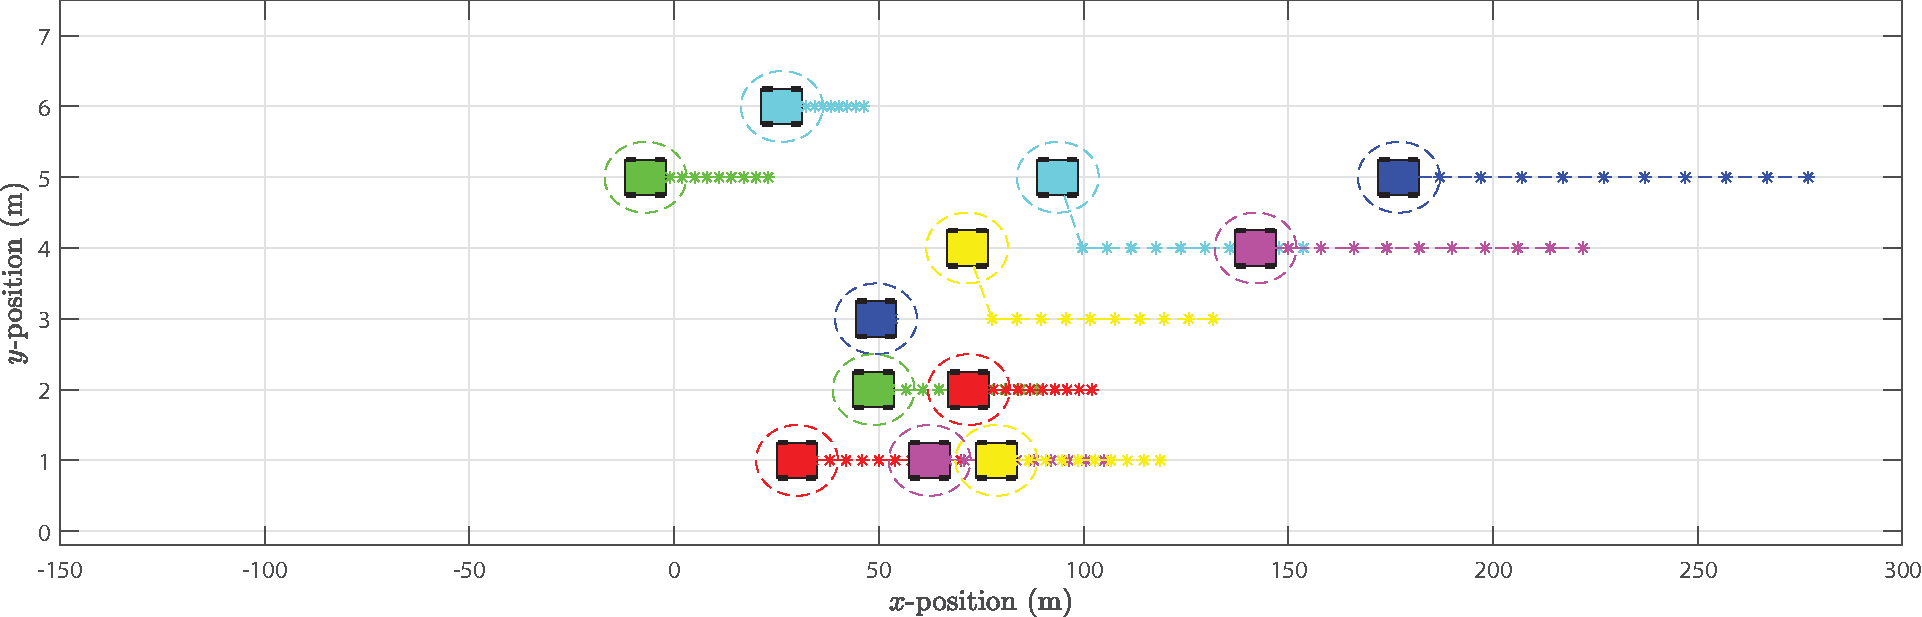
\includegraphics[width=\textwidth]{Kap6/obs_avoid/obs_avoid_traj40.eps}
    \caption{Predicted position at first position.}
    \label{fig:first}
\end{subfigure}
\vspace{1cm}
\begin{subfigure}[b]{0.45\textwidth}
    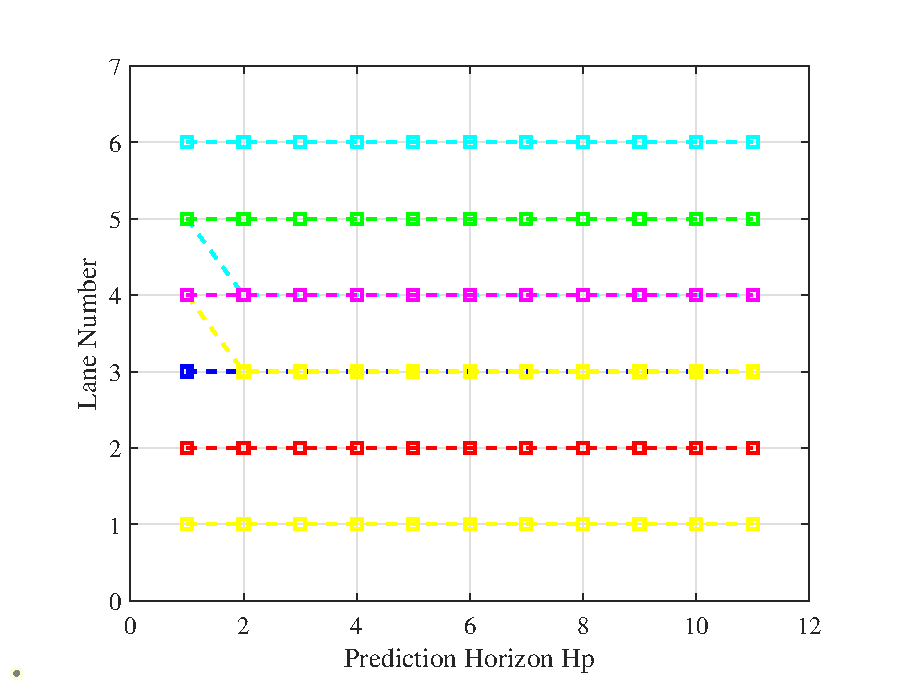
\includegraphics[width=\textwidth]{Kap6/obs_avoid/obs_avoid_lane40.eps}
    \caption{Predicted lane positions.}
    \label{fig:second}
\end{subfigure}
\hfill
\begin{subfigure}[b]{0.45\textwidth}
    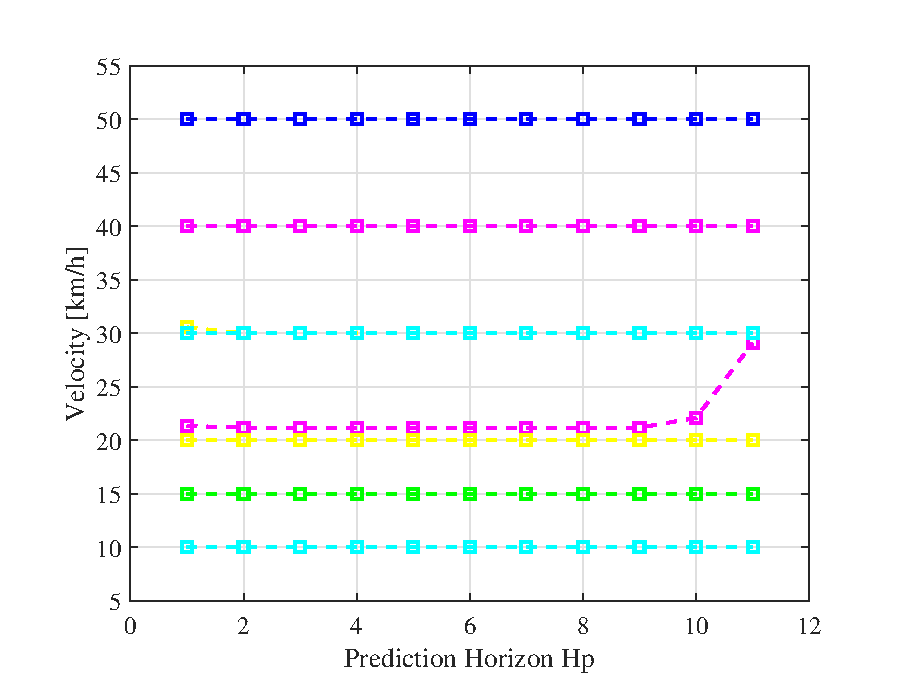
\includegraphics[width=\textwidth]{Kap6/obs_avoid/obs_avoid_vel40.eps}
    \caption{Predicted velocity profiles.}
    \label{fig:third}
\end{subfigure}
\caption{MPC Iteration = 30.}
\label{fig:figures}
\end{figure}
% .......................................
\begin{figure}[H]
\centering
    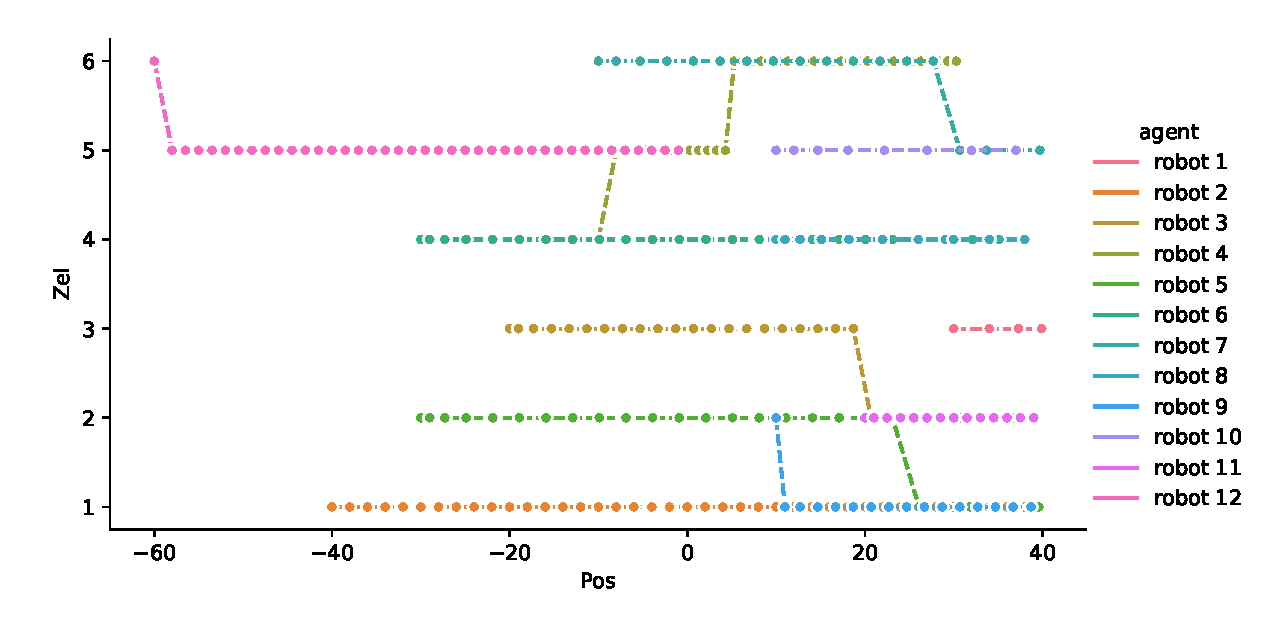
\includegraphics[width=0.8\textwidth]{Kap6/obs_avoid/obs_avoid_trajectories.eps}
    \caption{Trajectories of the entire network during the simulation time.}
\end{figure}

% ////////////////////////////


The simulation results show that the controller can provide a solution to obstacles that may arise Fig \ref{obs_avoid_step_time}. Also, the solution time of each of the sample steps is less in this scenario compared to the unconstrained scenario. This is due to the few interactions they have to do between vehicles after avoiding the obstacle vehicle. In addition, near step 10, it is possible to analyze the increase in solution time because in this step, the vehicles are dealing with the obstacle on the road.

\begin{figure}[H]
\centering
    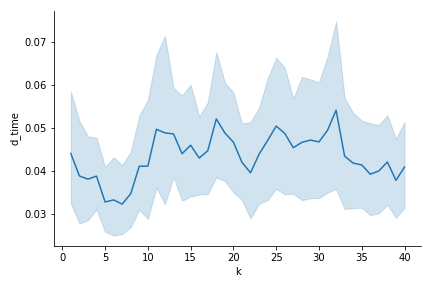
\includegraphics[width=.6\textwidth]{Kap6/obs_avoid/obs_avoid_d_time.png}
    \caption{Step Time}
    \label{obs_avoid_step_time}
\end{figure}

% ...........................

In the time analysis, depending on the prediction horizon, it can be seen that despite reaching 12 prediction steps, the system can provide a reasonable solution with a good time. In any case, the controller sometimes fails to find a minimum due to the big number of constraints.



\begin{figure}[H]
\centering
    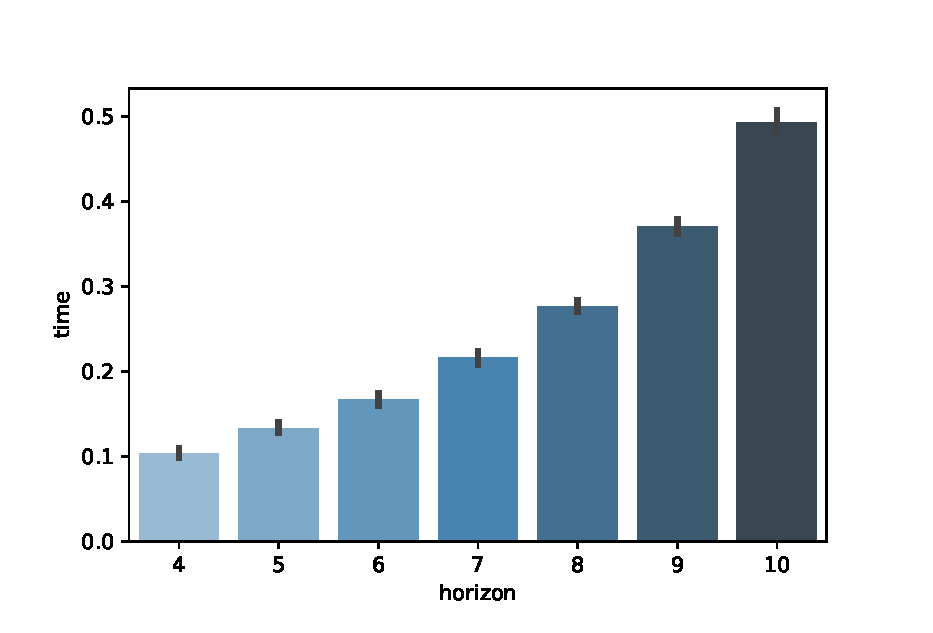
\includegraphics[width=0.6\textwidth]{Kap6/obs_avoid/obs_avoid_horizon_time.eps}
    \caption{Non-linear model of a differential robot.}
    % \label{kinematic2}
\end{figure}

Finally, as in the previous scenario, the difference in solving time is appreciated as the number of agents in the network increases. However, unlike the previous scenario, the D-MPC increases its duration with more vehicles.




\begin{figure}[H]
\centering
    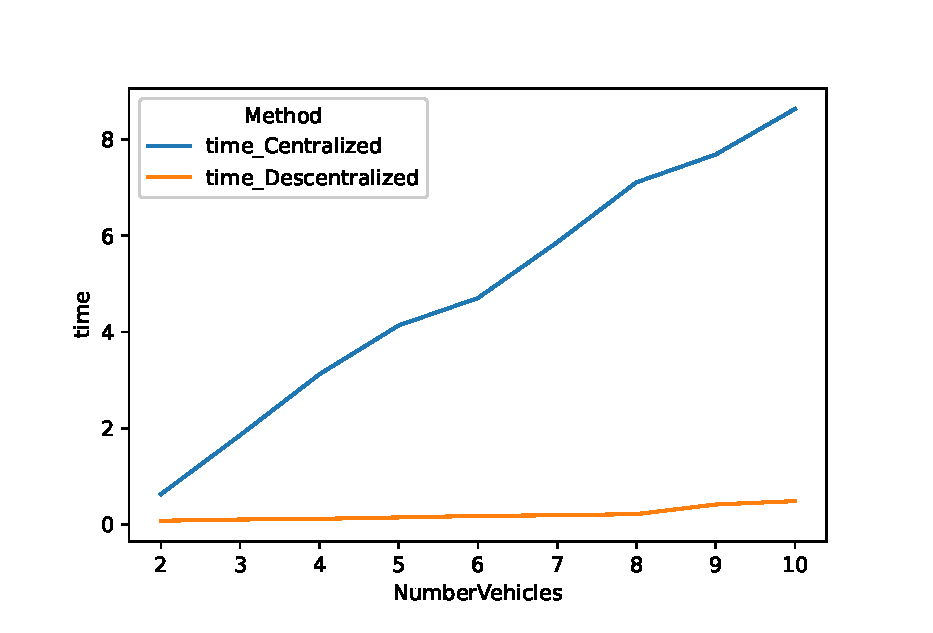
\includegraphics[width=0.6\textwidth]{Kap6/obs_avoid/obs_avoid_n_vehicles.eps}

\end{figure}


\subsection{Conclusion Obstacle Avoidance Scenario}

In a real highway environment, if a vehicle or other obstacle appears on the road, the decisions made by other vehicles are crucial. For this reason, this scenario of obstacles on the road was analyzed. With this new scenario, the number of constraints and the number of communications that each of the vehicles must deal with is greater than usual.

\\
\\
The obstacle avoidance scenario simulation shows that both C-MPC and D-MPC manage to solve the autonomous driving problem despite the increase in its constraints and a significant increase in communications between vehicles for the D-MPC case. However, the C-MPC continues to have difficulties providing an optimal solution in many evaluation cases. The system fell into an infeasible position causing the entire network to crash. This is because the solution algorithm that is used by the optimization engine (branch and bound) solves the problem by trying multiple possible solutions. While this is powerful, it can also be marginally unstable. The D-MPC manages to deal with the increase in constraints properly. However, more than the solution time is needed to be able to be implemented in real-time.

% \subsection{}

\newpage
% -------------------------------------------
\section{Reduced Scenario}
% -------------------------------------------

The reduced avoidance scenario was designed with 12 vehicles on the same road. It also has six lanes in line, and the road is one-way. There is a reduction in the number of lanes from 6 to 1. At a distance of 150 cm, the change starts. The main objective is to emulate a scenario where construction or change of the highway could happen. Moreover, it is an excellent opportunity to test the controller's behavior in the presence of a drastic change in its solution space. 

\begin{figure}[H]
\centering
\begin{subfigure}[t]{\textwidth}
    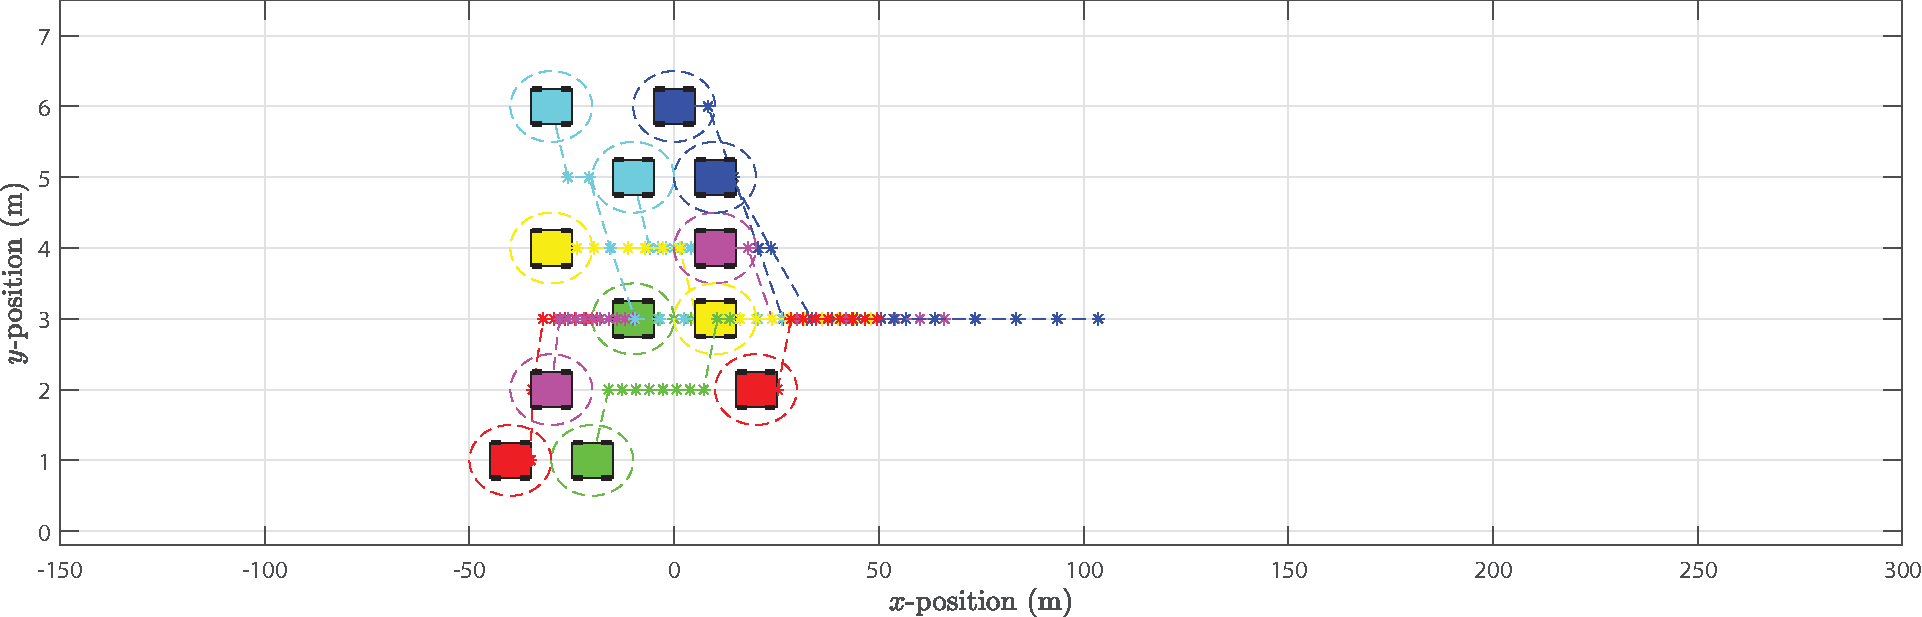
\includegraphics[width=\textwidth]{Kap6/red_lane/red_lane_traj0.eps}
    \caption{Predicted positions.}
    \label{fig:first}
\end{subfigure}
\vspace{1cm}
\begin{subfigure}[b]{0.45\textwidth}
    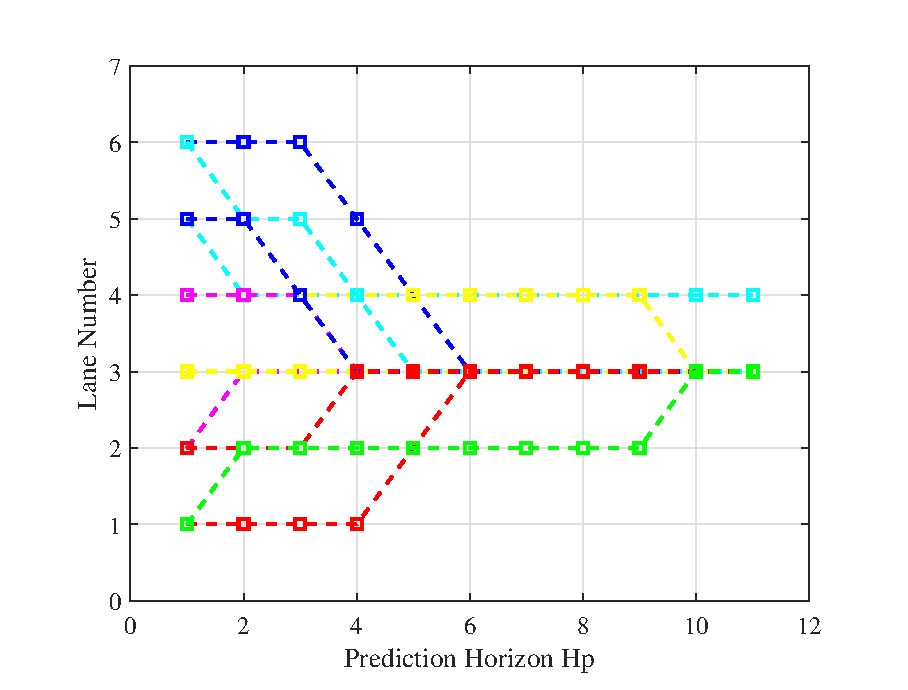
\includegraphics[width=\textwidth]{Kap6/red_lane/red_lane_lane0.eps}
    \caption{Predicted lane profiles.}
    \label{fig:second}
\end{subfigure}
\hfill
\begin{subfigure}[b]{0.45\textwidth}
    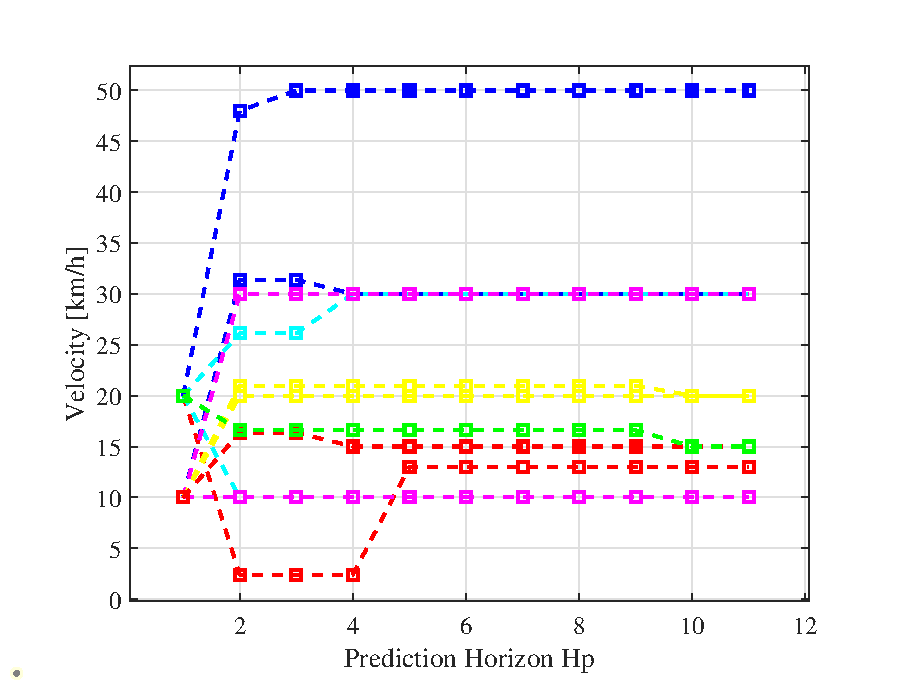
\includegraphics[width=\textwidth]{Kap6/red_lane/red_lane_vel0.eps}
    \caption{Predicted velocity profiles.}
    \label{fig:third}
\end{subfigure}
\caption{MPC Iteration = 0. Lane reduction scenario}
\label{fig:figures}
\end{figure}
\\
% ?.......................................
\begin{figure}[H]
\centering
\begin{subfigure}[t]{\textwidth}
    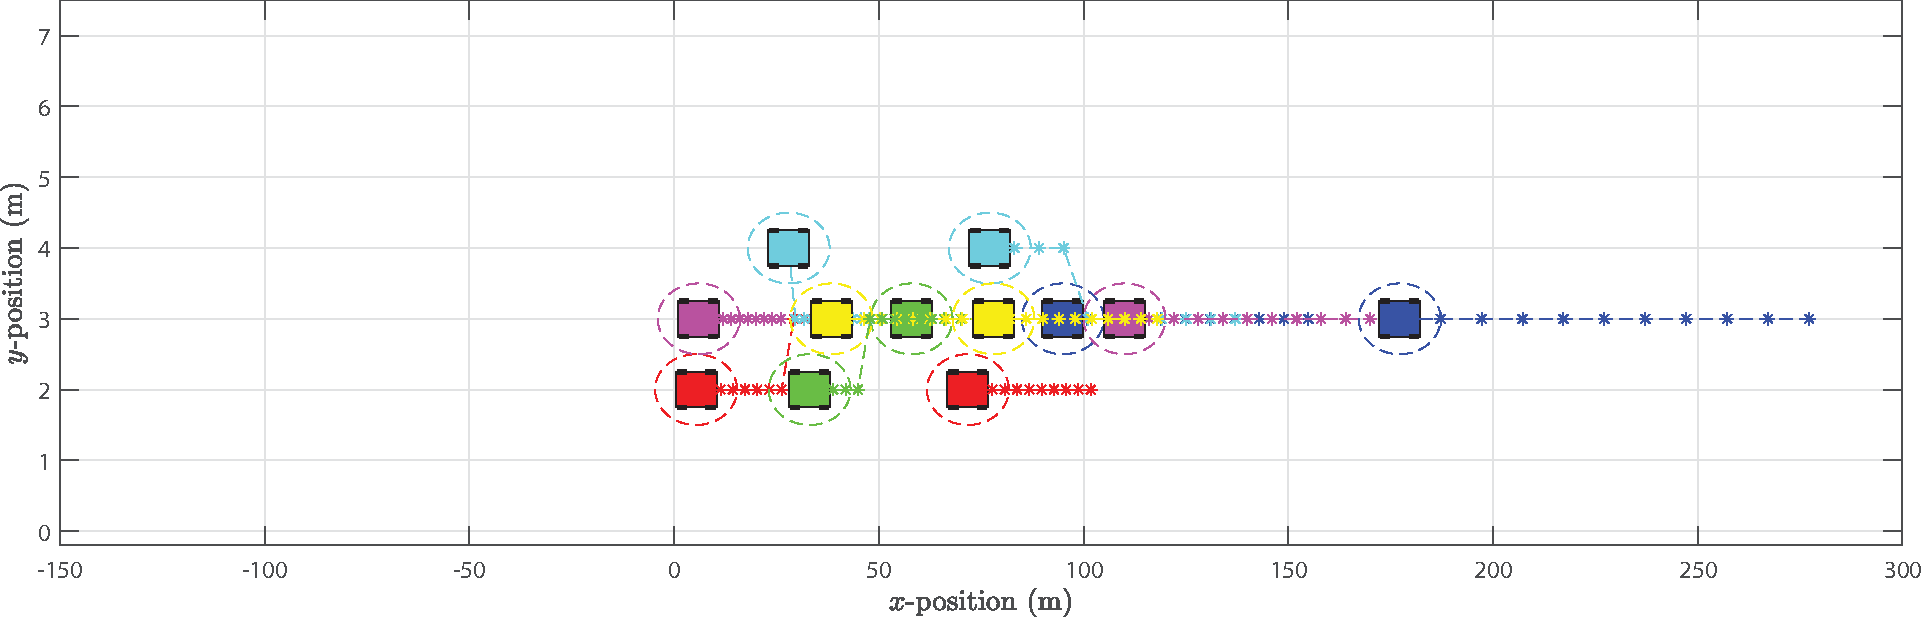
\includegraphics[width=\textwidth]{Kap6/red_lane/red_lane_traj10.eps}
    \caption{Predicted position.}
    \label{fig:first_mpc10_redsce}
\end{subfigure}
\vspace{1cm}
\begin{subfigure}[b]{0.45\textwidth}
    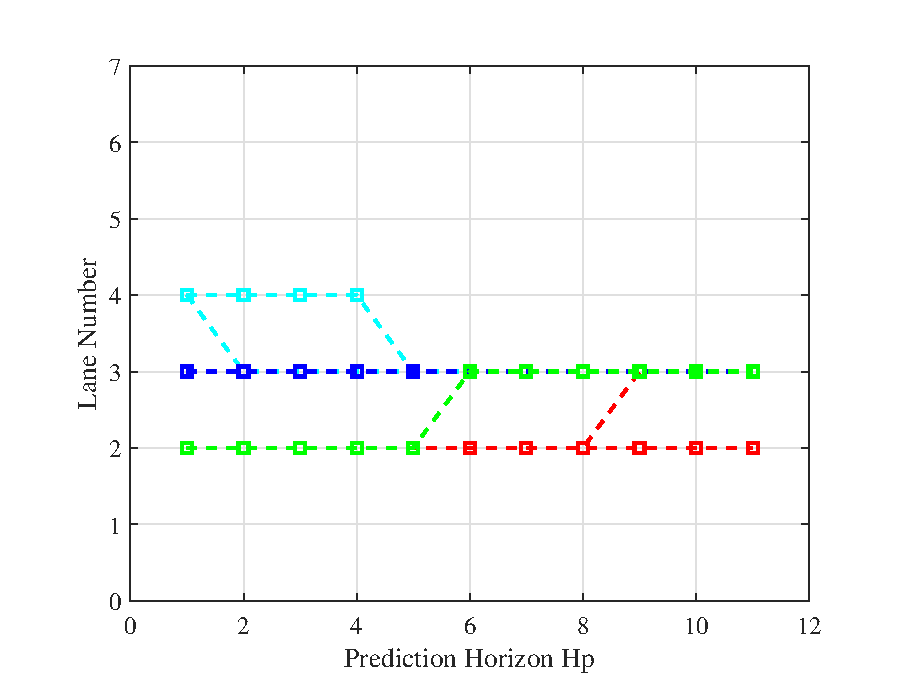
\includegraphics[width=\textwidth]{Kap6/red_lane/red_lane_lane10.eps}
    \caption{Predicted lane positions.}
    \label{fig:second}
\end{subfigure}
\hfill
\begin{subfigure}[b]{0.45\textwidth}
    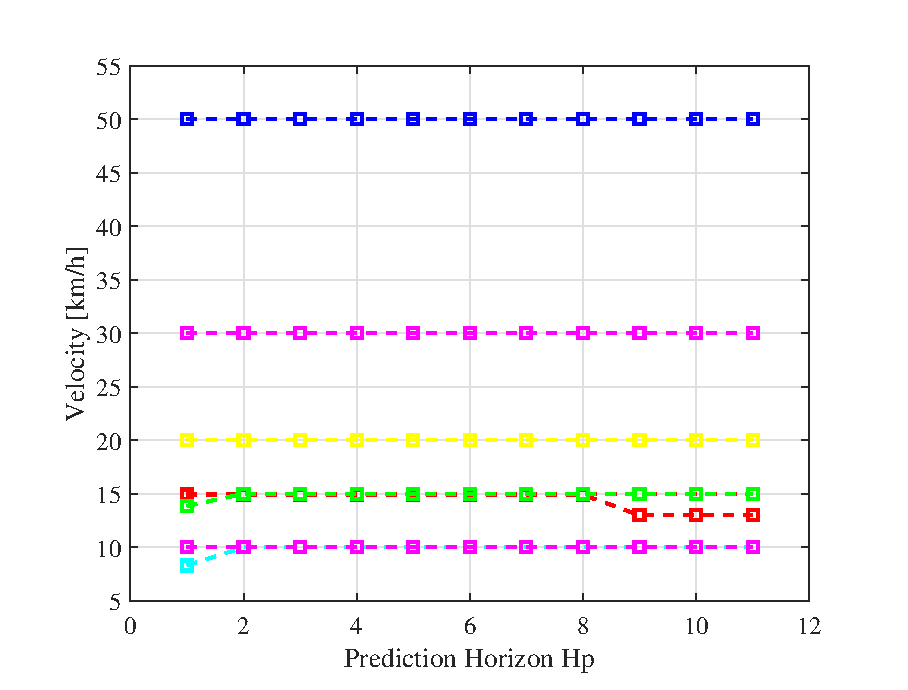
\includegraphics[width=\textwidth]{Kap6/red_lane/red_lane_vel10.eps}
    \caption{Predicted velocity profiles.}
    \label{fig:third_mpc10_redsce}
\end{subfigure}
\caption{MPC Iteration = 10. Lane reduction scenario}
\label{fig:figures}
\end{figure}
\\
Step 10 of the simulation in the reduced scenario shows how the vehicles have managed to occupy three lanes without colliding. In addition, fig  \ref{fig:first_mpc10_redsce} shows seven vehicles that have managed to occupy the central lane and five planning to occupy it. Moreover, it shows how they consider the speed, current position, and current lane to predict the future where they can enter lane three without colliding with the others.
\\

In fig \ref{fig:third_mpc10_redsce}, it is seen how most do not change their speed even though they may have different target speeds. This consensus is defined by the Game Theory Controller, where it is of greater importance to comply with the security regulations than to achieve the main objective for the controller.
\\



% .........................................
\begin{figure}[H]
\centering
\begin{subfigure}[t]{\textwidth}
    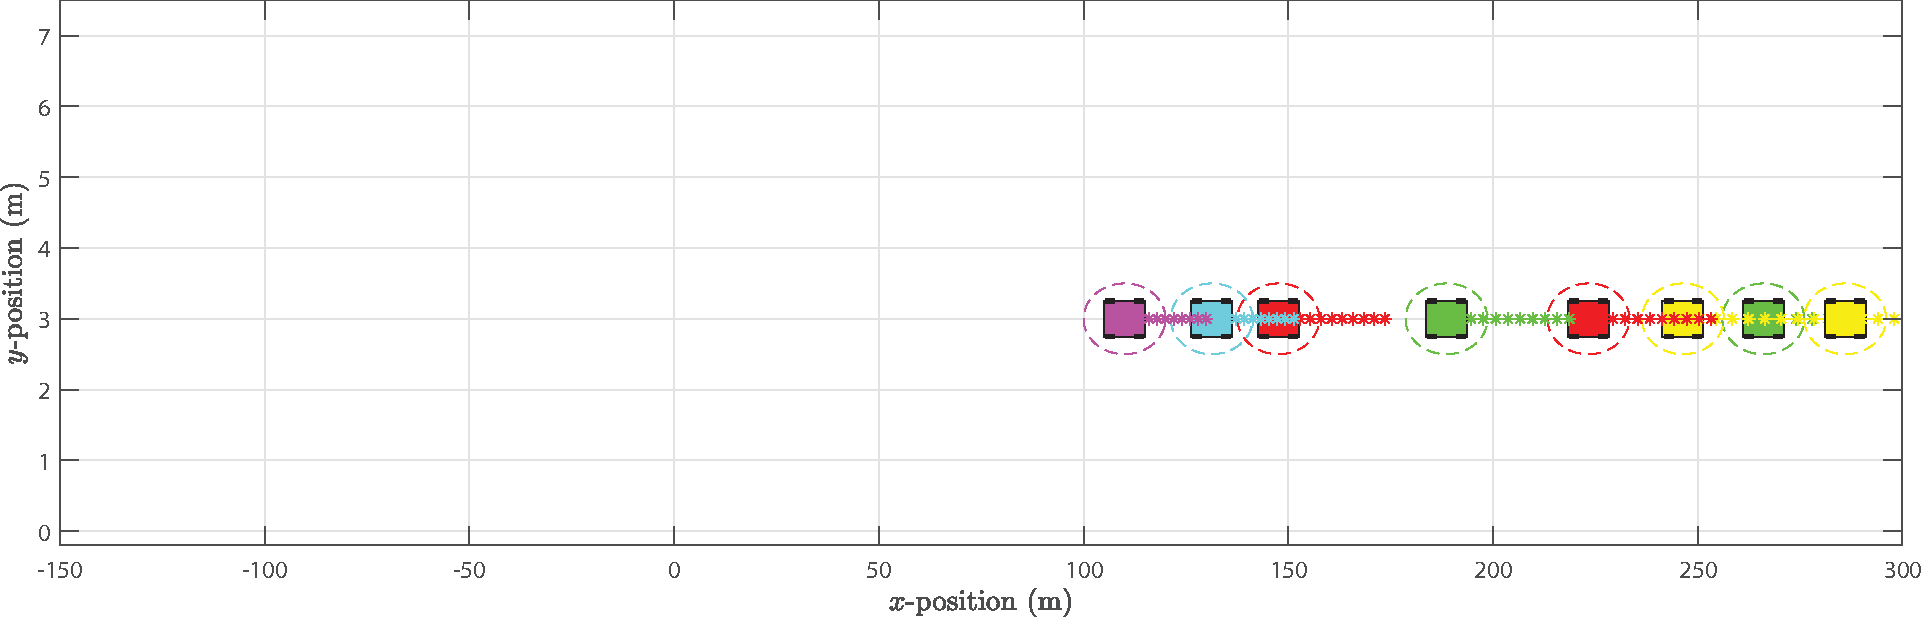
\includegraphics[width=\textwidth]{Kap6/red_lane/red_lane_traj36.eps}
    \caption{Predicted position at first position.}
    \label{fig:first}
\end{subfigure}
\vspace{1cm}
\begin{subfigure}[b]{0.45\textwidth}
    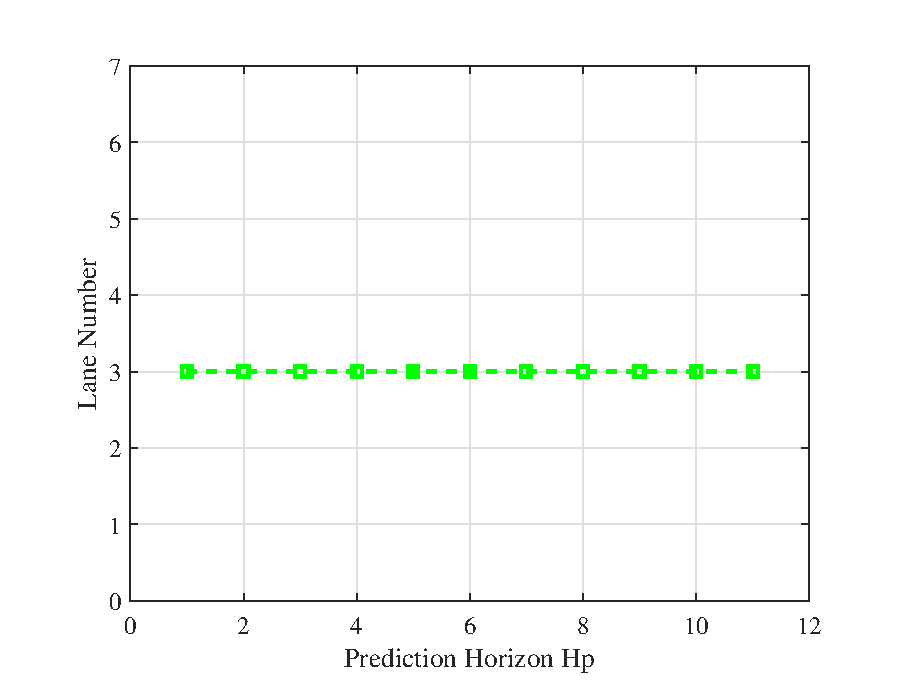
\includegraphics[width=\textwidth]{Kap6/red_lane/red_lane_lane36.eps}
    \caption{Predicted lane positions.}
    \label{fig:second}
\end{subfigure}
\hfill
\begin{subfigure}[b]{0.45\textwidth}
    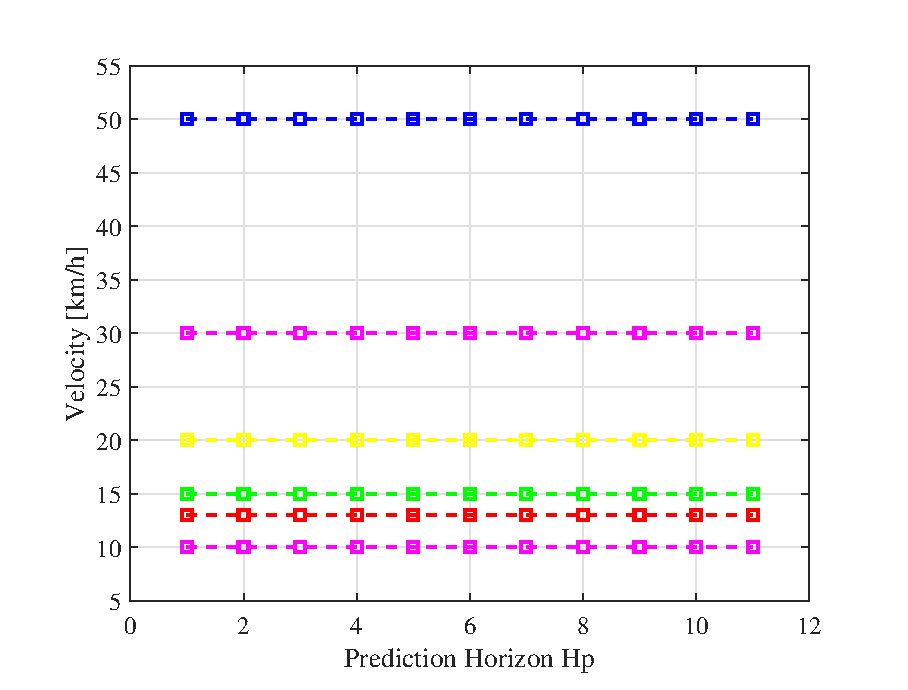
\includegraphics[width=\textwidth]{Kap6/red_lane/red_lane_vel36.eps}
    \caption{Predicted velocity profiles.}
    \label{fig:third}
\end{subfigure}
\caption{MPC Iteration = 30. Lane reduction scenario}
\label{fig:figures}
\end{figure}
% .......................................
\begin{figure}[H]
\centering
    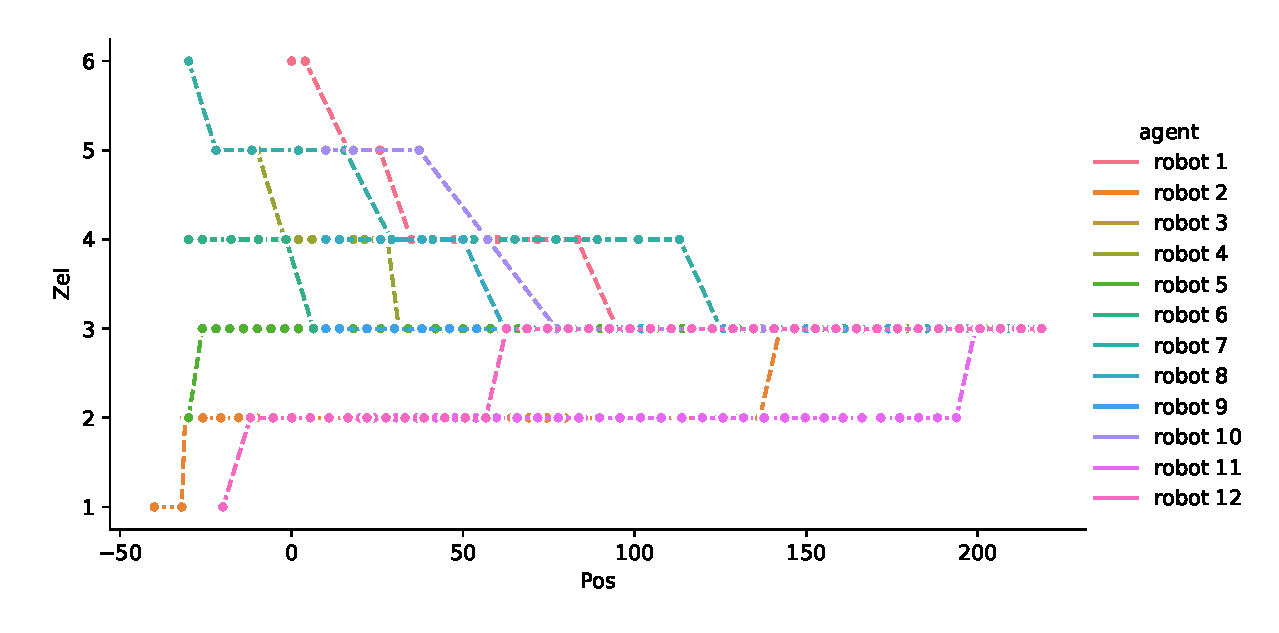
\includegraphics[width=0.8\textwidth]{Kap6/red_lane/red_lane_trajectories.eps}
    \caption{Trajectories of the entire network during the simulation time.}
    \label{red_lane_traject}
\end{figure}


Fig \ref{red_lane_traject} shows the trajectories travelled by vehicles as a result of a Generalized Potential Game control repeatedly solved by D-MPC for 12 vehicles. It is interesting to see how, despite the short space and time, 12 vehicles manage to synchronize to be able to enter the same lane without colliding and taking into account the decisions of the others. Also, the last vehicle $i=12$, is the last one that manages to join the lane. This is due to the initial conditions.

% ////////////////////////////

% {\color{blue} explicacion de como varian los tiempos de computo en cada iteracion  }

\begin{figure}[H]
\centering
    \includegraphics[width=.6\textwidth]{Kap6/red_lane/red_lane_d_time.png}
    \caption{Step Time}
    \label{red_lane_step_time}
\end{figure}

Figure \ref{red_lane_step_time} shows how the average solution time of the D-MPC is reduced by the reduction of restrictions and by the limited solution space. The network is at its maximum computation level at the simulation's beginning. This is due to the beginning, exist 12 vehicles trying to synchronize in order to be all on the same line.


\begin{figure}[H]
\centering
    \includegraphics[width=0.6\textwidth]{Kap6/red_lane/red_lane_horizon_time.eps}
    \caption{Non-linear model of a differential robot.}
    \label{red_lane_horizon}
\end{figure}

The same feasibility analysis was performed by increasing the prediction horizon, and the D-MPC was able to solve the OCP without problems, Fig \ref{red_lane_horizon}. This system does not represent an effort to the Generalized Potential games theorem due to its low level of interactions between vehicles at the end of the simulation.




\begin{figure}[H]
\centering
    \includegraphics[width=0.6\textwidth]{Kap6/red_lane/red_lane_n_vehicles.eps}

\end{figure}

Finally, in the comparison of the times of each of the architectures, the C-MPC has an exponential increase in its solution time. The reduction of interactions does not significantly favor the centralized architecture. However, the D-MPC manages to maintain the average time of the complete simulation regardless of the increase in vehicles. This is due to the fact that the $\epsilon$-Nash equilibrium can be solved more quickly, and the OCP problem is reduced to the interaction of each vehicle with the vehicle in front and behind.

\subsection{Conclusion Reduced Scenario}

One of the scenarios that a vehicle could face on a highway would be that of construction on the road. This new change in the road conditions would be reflected in the set of spatial variables $\mathcal{L}$, which would be reduced from 6 to 1. We trust that the GMIPG in a D-MPC architecture shown in this thesis document can deal with this problem.
\\

\\
In C-MPC, when vehicles are merging into a single lane, it is difficult for them to find an optimal decision to avoid colliding with each other. With an increase in the prediction horizon, this inconvenience could be solved. However, it is not what was expected.
In D-MPC, the solution was always possible regardless of the prediction horizon used. In addition, the solution time could be reduced as each of the vehicles adhered to the single lane. This is because there are fewer connections that each agent must take into account to provide an optimal solution.
\\

In short, the C-MPC fails to give an adequate response to the problem of driving on a freeway with a lane reduction and in front of selfish agents trying to join the same lane. However, the D-MPC controller manages to deal with this problem with improved solution time and does not have problems with the solutions. See fig \ref{red_lane_step_time} .
The reduced scenario was chosen to analyze the behavior of both drivers in the face of a sudden reduction, such as the lanes of a highway. See fig \ref{red_lane_traject}. All vehicles manage to synchronize to be able to stay in a single lane.

\chapter{Implementation}


\section{Unrestricted Scenario}
\begin{figure}
\centering
\begin{subfigure}[t]{\textwidth}
    \includegraphics[width=\textwidth]{Kap7/no_restricted/no_res_it0_cam0.png}
    \caption{Controller vision.}
    \label{fig:first}
\end{subfigure}
\vspace{1cm}
\begin{subfigure}[b]{0.4\textwidth}
    \includegraphics[width=\textwidth]{Kap7/no_restricted/no_res_it0_cam1.png}
    \caption{Front Vision.}
    \label{fig:second}
\end{subfigure}
\hfill
\begin{subfigure}[b]{0.50\textwidth}
    \includegraphics[width=\textwidth]{Kap7/no_restricted/no_res_it0_cam2.png}
    \caption{Lateral vision.}
    \label{fig:third}
\end{subfigure}
\caption{Implementation at iteration 0.}
\label{fig:figures}
\end{figure}




% \chapter{Implementation}

\begin{figure}
\centering
\begin{subfigure}[t]{\textwidth}
    \includegraphics[width=\textwidth]{Kap7/no_restricted/no_res_it10_cam0.png}
    \caption{Controller vision.}
    \label{fig:first}
\end{subfigure}
\vspace{1cm}
\begin{subfigure}[b]{0.4\textwidth}
    \includegraphics[width=\textwidth]{Kap7/no_restricted/no_res_it10_cam1.png}
    \caption{Front Vision.}
    \label{fig:second}
\end{subfigure}
\hfill
\begin{subfigure}[b]{0.50\textwidth}
    \includegraphics[width=\textwidth]{Kap7/no_restricted/no_res_it10_cam2.png}
    \caption{Lateral vision.}
    \label{fig:third}
\end{subfigure}
\caption{Implementation at iteration 10.}
\label{fig:figures}
\end{figure}




% \chapter{Implementation}

\begin{figure}
\centering
\begin{subfigure}[t]{\textwidth}
    \includegraphics[width=\textwidth]{Kap7/no_restricted/no_res_it30_cam0.png}
    \caption{Controller vision.}
    \label{fig:first}
\end{subfigure}
\vspace{1cm}
\begin{subfigure}[b]{0.4\textwidth}
    \includegraphics[width=\textwidth]{Kap7/no_restricted/no_res_it30_cam1.png}
    \caption{Front Vision.}
    \label{fig:second}
\end{subfigure}
\hfill
\begin{subfigure}[b]{0.50\textwidth}
    \includegraphics[width=\textwidth]{Kap7/no_restricted/no_res_it30_cam2.png}
    \caption{Lateral vision.}
    \label{fig:third}
\end{subfigure}
\caption{Implementation at iteration 30.}
\label{fig:figures}
\end{figure}
% ----------------------------------------
\section{Obstacle avoidance}

\begin{figure}
\centering
\begin{subfigure}[t]{\textwidth}
    \includegraphics[width=\textwidth]{Kap7/obs_avoid/obs_avoid_it0_cam0.png}
    \caption{Controller vision.}
    \label{fig:first}
\end{subfigure}
\vspace{1cm}
\begin{subfigure}[b]{0.4\textwidth}
    \includegraphics[width=\textwidth]{Kap7/obs_avoid/obs_avoid_it0_cam1.png}
    \caption{Front Vision.}
    \label{fig:second}
\end{subfigure}
\hfill
\begin{subfigure}[b]{0.50\textwidth}
    \includegraphics[width=\textwidth]{Kap7/obs_avoid/obs_avoid_it0_cam2.png}
    \label{fig:third}
\end{subfigure}
\caption{Implementation at iteration 0.}
\label{fig:figures}
\end{figure}




% \chapter{Implementation}

\begin{figure}
\centering
\begin{subfigure}[t]{\textwidth}
    \includegraphics[width=\textwidth]{Kap7/obs_avoid/obs_avoid_it10_cam0.png}
    \caption{Controller vision.}
    \label{fig:first}
\end{subfigure}
\vspace{1cm}
\begin{subfigure}[b]{0.4\textwidth}
    \includegraphics[width=\textwidth]{Kap7/obs_avoid/obs_avoid_it10_cam1.png}
    \caption{Front Vision.}
    \label{fig:second}
\end{subfigure}
\hfill
\begin{subfigure}[b]{0.50\textwidth}
    \includegraphics[width=\textwidth]{Kap7/obs_avoid/obs_avoid_it10_cam2.png}
    \caption{Lateral vision.}
    \label{fig:third}
\end{subfigure}
\caption{Implementation at iteration 10.}
\label{fig:figures}
\end{figure}




% \chapter{Implementation}

\begin{figure}
\centering
\begin{subfigure}[t]{\textwidth}
    \includegraphics[width=\textwidth]{Kap7/obs_avoid/obs_avoid_it40_cam0.png}
    \caption{Controller vision.}
    \label{fig:first}
\end{subfigure}
\vspace{1cm}
\begin{subfigure}[b]{0.4\textwidth}
    \includegraphics[width=\textwidth]{Kap7/obs_avoid/obs_avoid_it40_cam1.png}
    \caption{Front Vision.}
    \label{fig:second}
\end{subfigure}
\hfill
\begin{subfigure}[b]{0.50\textwidth}
    \includegraphics[width=\textwidth]{Kap7/obs_avoid/obs_avoid_it40_cam2.png}
    \caption{Lateral vision.}
    \label{fig:third}
\end{subfigure}
\caption{Implementation at iteration 40.}
\label{fig:figures}
\end{figure}




\section{Reduced Scenario}

\begin{figure}
\centering
\begin{subfigure}[t]{\textwidth}
    \includegraphics[width=\textwidth]{Kap7/red_lane/red_lane_it0_cam0.png}
    \caption{Controller vision.}
    \label{fig:first}
\end{subfigure}
\vspace{1cm}
\begin{subfigure}[b]{0.4\textwidth}
    \includegraphics[width=\textwidth]{Kap7/red_lane/red_lane_it0_cam1.png}
    \caption{Front Vision.}
    \label{fig:second}
\end{subfigure}
\hfill
\begin{subfigure}[b]{0.50\textwidth}
    \includegraphics[width=\textwidth]{Kap7/red_lane/red_lane_it0_cam2.png}
    \label{fig:third}
\end{subfigure}
\caption{Implementation at iteration 0.}
\label{fig:figures}
\end{figure}




% \chapter{Implementation}

\begin{figure}
\centering
\begin{subfigure}[t]{\textwidth}
    \includegraphics[width=\textwidth]{Kap7/red_lane/red_lane_it10_cam0.png}
    \caption{Controller vision.}
    \label{fig:first}
\end{subfigure}
\vspace{1cm}
\begin{subfigure}[b]{0.4\textwidth}
    \includegraphics[width=\textwidth]{Kap7/obs_avoid/obs_avoid_it10_cam1.png}
    \caption{Front Vision.}
    \label{fig:second}
\end{subfigure}
\hfill
\begin{subfigure}[b]{0.50\textwidth}
    \includegraphics[width=\textwidth]{Kap7/red_lane/red_lane_it10_cam2.png}
    \caption{Lateral vision.}
    \label{fig:third}
\end{subfigure}
\caption{Implementation at iteration 10.}
\label{fig:figures}
\end{figure}




% \chapter{Implementation}

\begin{figure}
\centering
\begin{subfigure}[t]{\textwidth}
    \includegraphics[width=\textwidth]{Kap7/red_lane/red_lane_it40_cam0.png}
    \caption{Controller vision.}
    \label{fig:first}
\end{subfigure}
\vspace{1cm}
\begin{subfigure}[b]{0.4\textwidth}
    \includegraphics[width=\textwidth]{Kap7/red_lane/red_lane_it40_cam1.png}
    \caption{Front Vision.}
    \label{fig:second}
\end{subfigure}
\hfill
\begin{subfigure}[b]{0.50\textwidth}
    \includegraphics[width=\textwidth]{Kap7/red_lane/red_lane_it40_cam2.png}
    \caption{Lateral vision.}
    \label{fig:third}
\end{subfigure}
\caption{Implementation at iteration 40.}
\label{fig:figures}
\end{figure}
\begin{appendix}
\label{AnexoA}

\chapter{Annex: Implementation Images}

In addition to simulations, the complete system was implemented in a testbed system \cite{agrobots}. Below are the images taken in the implementation of each of the scenarios analyzed in this document.

\section{Unrestricted Scenario}
\begin{figure}[H]
\centering
\begin{subfigure}[t]{\textwidth}
    \includegraphics[width=\textwidth]{Anexos/no_restricted/no_res_it0_cam0.png}
    \caption{Controller vision.}
    \label{fig:first}
\end{subfigure}
\vspace{1cm}
\begin{subfigure}[b]{0.4\textwidth}
    \includegraphics[width=\textwidth]{Anexos/no_restricted/no_res_it0_cam1.png}
    \caption{Front Vision.}
    \label{fig:second}
\end{subfigure}
\hfill
\begin{subfigure}[b]{0.50\textwidth}
    \includegraphics[width=\textwidth]{Anexos/no_restricted/no_res_it0_cam2.png}
    \caption{Lateral vision.}
    \label{fig:third}
\end{subfigure}
\caption{Implementation at iteration 0.}
\label{fig:figures}
\end{figure}




% \chapter{Implementation}

\begin{figure}[H]
\centering
\begin{subfigure}[t]{\textwidth}
    \includegraphics[width=\textwidth]{Anexos/no_restricted/no_res_it10_cam0.png}
    \caption{Controller vision.}
    \label{fig:first}
\end{subfigure}
\vspace{1cm}
\begin{subfigure}[b]{0.4\textwidth}
    \includegraphics[width=\textwidth]{Anexos/no_restricted/no_res_it10_cam1.png}
    \caption{Front Vision.}
    \label{fig:second}
\end{subfigure}
\hfill
\begin{subfigure}[b]{0.50\textwidth}
    \includegraphics[width=\textwidth]{Anexos/no_restricted/no_res_it10_cam2.png}
    \caption{Lateral vision.}
    \label{fig:third}
\end{subfigure}
\caption{Implementation at iteration 10.}
\label{fig:figures}
\end{figure}




% \chapter{Implementation}

\begin{figure}[H]
\centering
\begin{subfigure}[t]{\textwidth}
    \includegraphics[width=\textwidth]{Anexos/no_restricted/no_res_it30_cam0.png}
    \caption{Controller vision.}
    \label{fig:first}
\end{subfigure}
\vspace{1cm}
\begin{subfigure}[b]{0.4\textwidth}
    \includegraphics[width=\textwidth]{Anexos/no_restricted/no_res_it30_cam1.png}
    \caption{Front Vision.}
    \label{fig:second}
\end{subfigure}
\hfill
\begin{subfigure}[b]{0.50\textwidth}
    \includegraphics[width=\textwidth]{Anexos/no_restricted/no_res_it30_cam2.png}
    \caption{Lateral vision.}
    \label{fig:third}
\end{subfigure}
\caption{Implementation at iteration 30.}
\label{fig:figures}
\end{figure}
% ----------------------------------------
\section{Obstacle avoidance}

\begin{figure}[H]
\centering
\begin{subfigure}[t]{\textwidth}
    \includegraphics[width=\textwidth]{Anexos/obs_avoid/obs_avoid_it0_cam0.png}
    \caption{Controller vision.}
    \label{fig:first}
\end{subfigure}
\vspace{1cm}
\begin{subfigure}[b]{0.4\textwidth}
    \includegraphics[width=\textwidth]{Anexos/obs_avoid/obs_avoid_it0_cam1.png}
    \caption{Front Vision.}
    \label{fig:second}
\end{subfigure}
\hfill
\begin{subfigure}[b]{0.50\textwidth}
    \includegraphics[width=\textwidth]{Anexos/obs_avoid/obs_avoid_it0_cam2.png}
    \label{fig:third}
\end{subfigure}
\caption{Implementation at iteration 0.}
\label{fig:figures}
\end{figure}




% \chapter{Implementation}

\begin{figure}[H]
\centering
\begin{subfigure}[t]{\textwidth}
    \includegraphics[width=\textwidth]{Anexos/obs_avoid/obs_avoid_it10_cam0.png}
    \caption{Controller vision.}
    \label{fig:first}
\end{subfigure}
\vspace{1cm}
\begin{subfigure}[b]{0.4\textwidth}
    \includegraphics[width=\textwidth]{Anexos/obs_avoid/obs_avoid_it10_cam1.png}
    \caption{Front Vision.}
    \label{fig:second}
\end{subfigure}
\hfill
\begin{subfigure}[b]{0.50\textwidth}
    \includegraphics[width=\textwidth]{Anexos/obs_avoid/obs_avoid_it10_cam2.png}
    \caption{Lateral vision.}
    \label{fig:third}
\end{subfigure}
\caption{Implementation at iteration 10.}
\label{fig:figures}
\end{figure}




% \chapter{Implementation}

\begin{figure}[H]
\centering
\begin{subfigure}[t]{\textwidth}
    \includegraphics[width=\textwidth]{Anexos/obs_avoid/obs_avoid_it40_cam0.png}
    \caption{Controller vision.}
    \label{fig:first}
\end{subfigure}
\vspace{1cm}
\begin{subfigure}[b]{0.4\textwidth}
    \includegraphics[width=\textwidth]{Anexos/obs_avoid/obs_avoid_it40_cam1.png}
    \caption{Front Vision.}
    \label{fig:second}
\end{subfigure}
\hfill
\begin{subfigure}[b]{0.50\textwidth}
    \includegraphics[width=\textwidth]{Anexos/obs_avoid/obs_avoid_it40_cam2.png}
    \caption{Lateral vision.}
    \label{fig:third}
\end{subfigure}
\caption{Implementation at iteration 40.}
\label{fig:figures}
\end{figure}




\section{Reduced Scenario}

\begin{figure}[H]
\centering
\begin{subfigure}[t]{\textwidth}
    \includegraphics[width=\textwidth]{Anexos/red_lane/red_lane_it0_cam0.png}
    \caption{Controller vision.}
    \label{fig:first}
\end{subfigure}
\vspace{1cm}
\begin{subfigure}[b]{0.4\textwidth}
    \includegraphics[width=\textwidth]{Anexos/red_lane/red_lane_it0_cam1.png}
    \caption{Front Vision.}
    \label{fig:second}
\end{subfigure}
\hfill
\begin{subfigure}[b]{0.50\textwidth}
    \includegraphics[width=\textwidth]{Anexos/red_lane/red_lane_it0_cam2.png}
    \label{fig:third}
\end{subfigure}
\caption{Implementation at iteration 0.}
\label{fig:figures}
\end{figure}




% \chapter{Implementation}

\begin{figure}[H]
\centering
\begin{subfigure}[t]{\textwidth}
    \includegraphics[width=\textwidth]{Anexos/red_lane/red_lane_it10_cam0.png}
    \caption{Controller vision.}
    \label{fig:first}
\end{subfigure}
\vspace{1cm}
\begin{subfigure}[b]{0.4\textwidth}
    \includegraphics[width=\textwidth]{Anexos/obs_avoid/obs_avoid_it10_cam1.png}
    \caption{Front Vision.}
    \label{fig:second}
\end{subfigure}
\hfill
\begin{subfigure}[b]{0.50\textwidth}
    \includegraphics[width=\textwidth]{Anexos/red_lane/red_lane_it10_cam2.png}
    \caption{Lateral vision.}
    \label{fig:third}
\end{subfigure}
\caption{Implementation at iteration 10.}
\label{fig:figures}
\end{figure}




% \chapter{Implementation}

\begin{figure}[H]
\centering
\begin{subfigure}[t]{\textwidth}
    \includegraphics[width=\textwidth]{Anexos/red_lane/red_lane_it40_cam0.png}
    \caption{Controller vision.}
    \label{fig:first}
\end{subfigure}
\vspace{1cm}
\begin{subfigure}[b]{0.4\textwidth}
    \includegraphics[width=\textwidth]{Anexos/red_lane/red_lane_it40_cam1.png}
    \caption{Front Vision.}
    \label{fig:second}
\end{subfigure}
\hfill
\begin{subfigure}[b]{0.50\textwidth}
    \includegraphics[width=\textwidth]{Anexos/red_lane/red_lane_it40_cam2.png}
    \caption{Lateral vision.}
    \label{fig:third}
\end{subfigure}
\caption{Implementation at iteration 40.}
\label{fig:figures}
\end{figure}


\end{appendix}
\addcontentsline{toc}{chapter}{\numberline{}Bibliograf\'{\i}a}
%\bibliographystyle{apalike}
\bibliographystyle{plaindin_esp}
\bibliography{BibliMSc}
\end{document}




